\ifdefined\latexbokFontdir\else\def\latexbokFontdir{../../fonts}\fi
\ifdefined\latexbokFiguredir\else\def\latexbokFiguredir{../../examples}\fi
\documentclass[lang=sv,ptsize=10pt,font=none,nomath,titles=bf,../../a4.tex]{subfiles}
\begin{document}
\section{Grafik med \LaTeX}\label{sec:4}
% Om att man behöver inkludera grafik, att man bör göra det i floats,
% etc.

\subsection{Vad är bra grafik?}
\subsubsection{Almänna tips}
\subsubsection{Programspecifika tips}
\subsubsubsection*{Bra \Rlogo-figurer med \texttt{ggplot2}}
\label{sec:ggplot2}
Standardgrafiken i \Rlogo är överlag ganska bra när det gäller statistisk
analys, men bristande på andra områden. På många sätt är det dessutom 
svårt att göra lite mer involverade saker som att ändra färger, sätta
ordentliga axlar, enheter och så vidare. \Rlogo-paketet \texttt{ggplot2}
skapades för att åtgärda detta, och skapar snyggare grafer på enklare
sätt.

Paketet är intuitivt och baserat på logiska kopplingar mellan data och
grafiska element, vilket gör att man kan bygga grafik genom att tänka
på datans innebörd och vad man vill kommunicera, istället för själva 
grafiken. En bra sammanfattning av paketet, som gör sig bäst på
originalspråket, är \foreignquote{british}{makes doing the right thing
easy, while keeping harder things possible}.

Att installera och använda \texttt{ggplot2} är enkelt. Efter att ha 
installerat paketet genom att köra kommandot
\verb|install.packages("ggplot2")|
i \Rlogo använder man det genom att inkludera paketet och använda
funktionen \texttt{ggplot} i kombination med någon av paketets många
plot-funktioner. Man kan även kombinera olika grafer:
\begin{rcode}
require(ggplot2)
# Exempeldata
df <- data.frame(
+   trt = factor(c(1, 1, 2, 2)),
+   resp = c(1, 5, 3, 4), 
+   group = factor(c(1, 2, 1, 2)),
+   se = c(0.1, 0.3, 0.3, 0.2)
+) 
df2 <- df[c(1,3),] 
# Toppen/botten på errorbars
limits <- aes(ymax = resp + se, ymin=resp - se)
dodge <- position_dodge(width=0.9)
# Plotta!
p <- ggplot(df, aes(fill=group, y=resp, x=trt))
p + geom_bar(position=dodge) +
  + geom_errorbar(limits, position=dodge, width=0.25)
\end{rcode}

En mer utförlig referens över alla kommandon i \texttt{ggplot2} finns
på internet\footnote{\url{http://had.co.nz/ggplot2/}}, och en grundlig
genomgång ges av \textcite{Hadley09}.

\subsubsubsection*{Bättre \MATLAB-figurer}
% ???

\subsection{Inkludera grafik}
Att kunna inkludera grafik av olika slag i sitt dokument kan verka så
vitalt och grundläggande att det rimligtvis inte bör finnas många olika
möjligheter. Så är dock inte fallet. Under den långa tid som \LaTeX{} har
existerat (och utvecklats) har en rad olika metoder för att inkludera
grafik, alla med specifika för- och nackdelar, utvecklats för systemet.

I grunden kan man dock dela upp dessa metoder i två undergrupper: de
paket som inkluderar grafik som skapats av externa program (till
exempel bilder i \PDF-, \PNG- eller \JPEG-format) och de som använder
funktionalitet i den underliggande \TeX-kompilatorn för att skapa grafik.

I den första kategorin finns i princip bara ett alternativ
--- \pack{graphicx}. Den senare kategorin har ett antal kandidater,
men för \pdfLaTeX\ och \XeTeX\ finns det en mycket stark kandidat:
\PGFTikZ. Båda dessa, samt deras för- och nackdelar, diskuteras nedan.

\subsubsection{Paketet \pack{graphicx}}
Den metod som oftast används, eftersom den kräver kortare
kompileringstider och mindre direkt ansträngning, är att inkludera
redan existerande bilder i \PDF- eller \PNG-format med hjälp av
paketet \pack{graphicx}. Paketet har ett mycket enkelt gränssnitt, och
har egentligen bara ett kommando av intresse: \cmd{includegraphics}.

Med hjälp av detta kommando kan man inkludera grafik av format som är
kompatibla med den \TeX-kompilator som används. I fallet \pdfLaTeX\ är
dessa format \PNG, \PDF\ och \JPEG. Kommandot tar ett valfritt
argument, en lista av nycklar, som används för att på olika sätt
skala om bilden som inkluderas, och ett obligatoriskt argument som
berättar var bilden finns:
\latex|\includegraphics[width=\textwidth]{filnamn}|
Fler sådana nycklar listas av \textcite[8\psq]{Carlisle05}.

Fördelen med denna metod är att den i princip \emph{alltid} fungerar,
eftersom nästan alla verktyg kan exportera \PNG- eller \PDF-filer (och
i de fall detta inte går kan man oftast konvertera till \PNG eller i
västa fall använda skärmdumpar). Metoden är såklart också bra för att
inkludera fotografier i \JPEG-format, till exempel bilder på
experimentuppställningar.

Nackdelen är att dessa format inte är vektorbaserade. Detta innebär att
om du behöver skala om bilden i efterhand, så kan grafiken bli suddig
eller otydlig. För till exempel linjediagram och liknande kan dessutom
texten på axlarna bli för liten eller otydlig, vilket såklart gör att
informationen inte kommuniceras lika effektivt. 

Sammanfattat kan man säga att \pack{graphicx} är utmärkt för att
inkludera \JPEG-bilder (dvs. fotografier), medans diagram, grafer och
liknande oftast blir bättre med \PGFTikZ eller \pack{pgfplots}.

\subsubsection{Rita med \PGFTikZ}
En metod som ofta ger bättre resultat, men som är lite mer avancerad att
använda (både eftersom den ger längre kompileringstider och eftersom den
kräver mer arbete av användaren) är att använda \PGFTikZ\ för att rita
den grafik som behövs.

\PGFTikZ\ är ett (mycket stort) paket som används för att rita
vektorgrafik direkt i \LaTeX. Paketet har en omfattande manual
\parencite{Tantau10} som innehåller många väldokumenterade exempel.
Dessutom ges en bra, kortfattad introduktion av \textcite{Mertz07}.
Använder man ett program som kan exportera \PGFTikZ-kod finns det oftast
ingen anledning att inte göra det, och i vissa fall (så som för enkla
figurer över uppställningar eller mekaniska figurer) kan det vara 
lättare att skriva \PGFTikZ-kod än att rita figuren i ett externt program.

Utöver de exempel som finns i manualen går det även att hitta mycket
material på internet\footnote{Bland annat så finns galleriet
\TeX{}ample.net\footref{fn:4:texample}, som innehåller 
många exempel på \PGFTikZ-kod, och taggen \emph{tikz-pgf} på
\TeX.SE\footref{fn:4:tex-se-tikz-pgf}, 
där man kan få svar på många frågor}. Ska man bara rita enkla grafer
finns dessutom det lite enklare paketet \pack{pgfplots}, som använder
\PGFTikZ\ internt (och som diskuteras nedan).%
\silentfootnote{\url{http://www.texample.net}\label{fn:4:texample}}%
\silentfootnote{\url{http://tex.stackexchange.com/questions/tagged/tikz-pgf}\label{fn:4:tex-se-tikz-pgf}}

Fördelen med \PGFTikZ ligger främst i det faktum att grafiken är
vektorbaserad, och därför ser lika bra ut oavsett hur mycket den skalas
om, samt att text i figuren behandlas av \LaTeX\ och därför kommer visas
i rätt typsnitt och vettiga storlekar vilket ökar läsbarheten i figuren.

Den främsta nackdelen är att \PGFTikZ-figurer ofta tar en stund att
kompilera, och att det inte alltid är möjligt att exportera figurer
i det formatet. \PGFTikZ-figurer är alltså att föredra för diagram,
grafer och liknande, men går inte att använda för till exempel
fotografier.

\subsubsubsection*{Plotta med \pack{pgfplots}}
Paketet \pack{pgfplots} kan sägas vara ett tillägg till \PGFTikZ som gör
det lättare att rita vanliga diagram (stapel- eller linjediagram, till
exempel) med hjälp av \PGFTikZ. Bland annat kan \pack{pgfplots} läsa in
data från externa filer och automatiskt omvandla den till figurer.

Paketet har en omfattande manual \parencite{Feuersanger13a}, som
detaljerat beskriver hur man använder paketet för att rita olika
sorters diagram.
Bland annat använder \texttt{matlab2tikz} — som diskuteras på
\cpageref{matlab2tikz} — funktionalitet från \pack{pgfplots}.
Det finns även ett påbyggnadspaket, \pack{pgfplotstable}
\parencite{Feuersanger13b}, som kan läsa
CSV-liknande filer och använda \pack{pgfplots} för att rita diagram
(och tabeller med \pack{booktabs}) utifrån dessa data.

\subsubsection{Varför hamnar figuren fel?}
% Hör inte detta hemma med floats i kapitel 2?

\subsection{Exportera grafik eller data}
När man väl skapat sin grafik i det program man arbetar med och är nöjd
med denna måste man exportera den till ett format som kan användas med
\LaTeX. Använder man \pdfLaTeX (vilket man bör) så stöds formaten \JPEG,
\PNG och \PDF. Av dessa lämpar sig \JPEG bäst till fotografier, medan
\PNG och \PDF lämpar sig väl till figurer och grafer.
Generellt sett är \PDF att föredra då formatet är vektorbaserat och
därför kan skalas både upp och ner utan att man förlorar någon kvalitet.

Om möjligheten finns är det bästa dock att exportera sina figurer som
\PGFTikZ-kod, vilket innebär att \LaTeX{} kommer att rendera dem och att
man därför har något större frihet när det gäller finjustering av figuren
i efterhand, och även att axlar och dylikt typsätts på samma sätt som
dokumentets brödtext vilket ger ett enhetligt intryck. Ett alternativ
till att exportera hela figurer som \PGFTikZ-kod är att exportera datan
i ett format som kan läsas av \pack{pgfplots}, och sedan använda det
paketet för att rita figurerna.

Det finns många (matematiska) programvaror, och det är orimligt att
inkludera instruktioner till alla i detta kapitel. Jag har därför valt
att beskriva hur man enklast exporterar figurer som \PGFTikZ-kod eller
i \PDF-format (i nödfall \PNG) från fyra vanliga programvaror:
\Rlogo, \MATLAB, \Mathematica och \gnuplot.

\subsubsection{Exportera i \PGFTikZ-format}
\PGFTikZ brukar inte vara ett format som normalt stöds av kommersiella
(eller fria) programvaror, och därför är funktionen ofta implementerad
som någon form av tillägg. Lyckligtvis brukar dessa vara öppna och fria
att använda för vem som helst.

\subsubsubsection*{Från \Rlogo med \texttt{tikzDevice}}
\Rlogo-paketet \texttt{tikzDevice} \parencite{Sharpsteen12} gör det möjligt
att i \Rlogo exportera figurer som \PGFTikZ-kod. Det kan som många andra
\Rlogo-paket hittas på CRAN och installeras enklast genom att köra
\Rlogo-kommandot \verb|install.packages("tikzDevice")|. Man använder
sedan kommandot \texttt{tikz} för att berätta för \Rlogo att grafiken
ska skrivas som \PGFTikZ-kod, och filen som skapas kan sedan inkluderas
i \LaTeX-dokument med kommandot \cmd{input}.
\Cref{ex:tikzdevice} visar resultatet av detta.

\begin{kod}[tbp]
	\centering
	\begin{minipage}{\textwidth}
		\centering
		% Created by tikzDevice version 0.6.2-80-b0c08dc on 2012-07-31 03:25:08
% !TEX encoding = UTF-8 Unicode
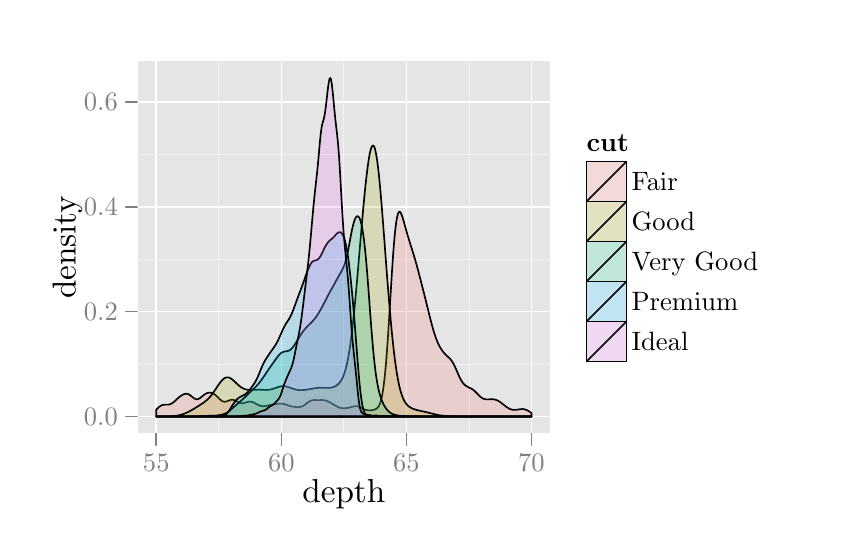
\begin{tikzpicture}[x=1pt,y=1pt]
\definecolor[named]{fillColor}{rgb}{1.00,1.00,1.00}
\path[use as bounding box,fill=fillColor,fill opacity=0.00] (0,0) rectangle (289.08,180.67);
\begin{scope}
\path[clip] (  0.00,  0.00) rectangle (289.08,180.67);
\definecolor[named]{fillColor}{rgb}{1.00,1.00,1.00}

\path[fill=fillColor] ( -0.00,  0.00) rectangle (289.08,180.68);
\end{scope}
\begin{scope}
\path[clip] (  0.00,  0.00) rectangle (289.08,180.67);
\definecolor[named]{drawColor}{rgb}{0.50,0.50,0.50}

\node[text=drawColor,anchor=base east,inner sep=0pt, outer sep=0pt, scale=  0.96] at ( 32.57, 36.85) {0.0};

\node[text=drawColor,anchor=base east,inner sep=0pt, outer sep=0pt, scale=  0.96] at ( 32.57, 74.75) {0.2};

\node[text=drawColor,anchor=base east,inner sep=0pt, outer sep=0pt, scale=  0.96] at ( 32.57,112.66) {0.4};

\node[text=drawColor,anchor=base east,inner sep=0pt, outer sep=0pt, scale=  0.96] at ( 32.57,150.57) {0.6};
\end{scope}
\begin{scope}
\path[clip] (  0.00,  0.00) rectangle (289.08,180.67);
\definecolor[named]{drawColor}{rgb}{0.50,0.50,0.50}

\path[draw=drawColor,line width= 0.6pt,line join=round,line cap=round] ( 35.42, 40.15) -- ( 39.69, 40.15);

\path[draw=drawColor,line width= 0.6pt,line join=round,line cap=round] ( 35.42, 78.06) -- ( 39.69, 78.06);

\path[draw=drawColor,line width= 0.6pt,line join=round,line cap=round] ( 35.42,115.97) -- ( 39.69,115.97);

\path[draw=drawColor,line width= 0.6pt,line join=round,line cap=round] ( 35.42,153.87) -- ( 39.69,153.87);
\end{scope}
\begin{scope}
\path[clip] ( 39.69, 34.03) rectangle (188.82,168.63);
\definecolor[named]{fillColor}{rgb}{0.90,0.90,0.90}

\path[fill=fillColor] ( 39.69, 34.03) rectangle (188.82,168.63);
\definecolor[named]{drawColor}{rgb}{0.95,0.95,0.95}

\path[draw=drawColor,line width= 0.3pt,line join=round,line cap=round] ( 39.69, 59.11) --
	(188.82, 59.11);

\path[draw=drawColor,line width= 0.3pt,line join=round,line cap=round] ( 39.69, 97.01) --
	(188.82, 97.01);

\path[draw=drawColor,line width= 0.3pt,line join=round,line cap=round] ( 39.69,134.92) --
	(188.82,134.92);

\path[draw=drawColor,line width= 0.3pt,line join=round,line cap=round] ( 69.06, 34.03) --
	( 69.06,168.63);

\path[draw=drawColor,line width= 0.3pt,line join=round,line cap=round] (114.25, 34.03) --
	(114.25,168.63);

\path[draw=drawColor,line width= 0.3pt,line join=round,line cap=round] (159.45, 34.03) --
	(159.45,168.63);
\definecolor[named]{drawColor}{rgb}{1.00,1.00,1.00}

\path[draw=drawColor,line width= 0.6pt,line join=round,line cap=round] ( 39.69, 40.15) --
	(188.82, 40.15);

\path[draw=drawColor,line width= 0.6pt,line join=round,line cap=round] ( 39.69, 78.06) --
	(188.82, 78.06);

\path[draw=drawColor,line width= 0.6pt,line join=round,line cap=round] ( 39.69,115.97) --
	(188.82,115.97);

\path[draw=drawColor,line width= 0.6pt,line join=round,line cap=round] ( 39.69,153.87) --
	(188.82,153.87);

\path[draw=drawColor,line width= 0.6pt,line join=round,line cap=round] ( 46.47, 34.03) --
	( 46.47,168.63);

\path[draw=drawColor,line width= 0.6pt,line join=round,line cap=round] ( 91.66, 34.03) --
	( 91.66,168.63);

\path[draw=drawColor,line width= 0.6pt,line join=round,line cap=round] (136.85, 34.03) --
	(136.85,168.63);

\path[draw=drawColor,line width= 0.6pt,line join=round,line cap=round] (182.04, 34.03) --
	(182.04,168.63);
\definecolor[named]{drawColor}{rgb}{0.00,0.00,0.00}
\definecolor[named]{fillColor}{rgb}{0.97,0.46,0.43}

\path[draw=drawColor,line width= 0.6pt,line join=round,line cap=round,fill=fillColor,fill opacity=0.20] ( 46.47, 42.65) --
	( 46.73, 42.92) --
	( 47.00, 43.18) --
	( 47.26, 43.42) --
	( 47.53, 43.65) --
	( 47.79, 43.85) --
	( 48.06, 44.02) --
	( 48.32, 44.16) --
	( 48.59, 44.27) --
	( 48.85, 44.35) --
	( 49.12, 44.40) --
	( 49.38, 44.43) --
	( 49.65, 44.45) --
	( 49.91, 44.45) --
	( 50.18, 44.45) --
	( 50.45, 44.45) --
	( 50.71, 44.46) --
	( 50.98, 44.49) --
	( 51.24, 44.55) --
	( 51.51, 44.62) --
	( 51.77, 44.73) --
	( 52.04, 44.86) --
	( 52.30, 45.03) --
	( 52.57, 45.22) --
	( 52.83, 45.43) --
	( 53.10, 45.66) --
	( 53.36, 45.90) --
	( 53.63, 46.15) --
	( 53.89, 46.41) --
	( 54.16, 46.65) --
	( 54.42, 46.89) --
	( 54.69, 47.12) --
	( 54.96, 47.34) --
	( 55.22, 47.54) --
	( 55.49, 47.72) --
	( 55.75, 47.89) --
	( 56.02, 48.03) --
	( 56.28, 48.15) --
	( 56.55, 48.25) --
	( 56.81, 48.33) --
	( 57.08, 48.37) --
	( 57.34, 48.38) --
	( 57.61, 48.35) --
	( 57.87, 48.29) --
	( 58.14, 48.18) --
	( 58.40, 48.04) --
	( 58.67, 47.87) --
	( 58.94, 47.67) --
	( 59.20, 47.46) --
	( 59.47, 47.24) --
	( 59.73, 47.03) --
	( 60.00, 46.84) --
	( 60.26, 46.67) --
	( 60.53, 46.54) --
	( 60.79, 46.45) --
	( 61.06, 46.41) --
	( 61.32, 46.42) --
	( 61.59, 46.48) --
	( 61.85, 46.59) --
	( 62.12, 46.73) --
	( 62.38, 46.91) --
	( 62.65, 47.11) --
	( 62.91, 47.33) --
	( 63.18, 47.55) --
	( 63.45, 47.77) --
	( 63.71, 47.98) --
	( 63.98, 48.17) --
	( 64.24, 48.34) --
	( 64.51, 48.48) --
	( 64.77, 48.60) --
	( 65.04, 48.69) --
	( 65.30, 48.75) --
	( 65.57, 48.78) --
	( 65.83, 48.78) --
	( 66.10, 48.76) --
	( 66.36, 48.71) --
	( 66.63, 48.63) --
	( 66.89, 48.53) --
	( 67.16, 48.40) --
	( 67.43, 48.24) --
	( 67.69, 48.05) --
	( 67.96, 47.84) --
	( 68.22, 47.60) --
	( 68.49, 47.35) --
	( 68.75, 47.08) --
	( 69.02, 46.81) --
	( 69.28, 46.55) --
	( 69.55, 46.30) --
	( 69.81, 46.08) --
	( 70.08, 45.88) --
	( 70.34, 45.72) --
	( 70.61, 45.60) --
	( 70.87, 45.53) --
	( 71.14, 45.50) --
	( 71.41, 45.52) --
	( 71.67, 45.56) --
	( 71.94, 45.64) --
	( 72.20, 45.73) --
	( 72.47, 45.84) --
	( 72.73, 45.94) --
	( 73.00, 46.04) --
	( 73.26, 46.12) --
	( 73.53, 46.18) --
	( 73.79, 46.20) --
	( 74.06, 46.20) --
	( 74.32, 46.16) --
	( 74.59, 46.09) --
	( 74.85, 45.99) --
	( 75.12, 45.86) --
	( 75.38, 45.73) --
	( 75.65, 45.58) --
	( 75.92, 45.43) --
	( 76.18, 45.29) --
	( 76.45, 45.17) --
	( 76.71, 45.07) --
	( 76.98, 45.00) --
	( 77.24, 44.95) --
	( 77.51, 44.94) --
	( 77.77, 44.95) --
	( 78.04, 45.00) --
	( 78.30, 45.06) --
	( 78.57, 45.14) --
	( 78.83, 45.23) --
	( 79.10, 45.32) --
	( 79.36, 45.40) --
	( 79.63, 45.47) --
	( 79.90, 45.52) --
	( 80.16, 45.54) --
	( 80.43, 45.54) --
	( 80.69, 45.51) --
	( 80.96, 45.45) --
	( 81.22, 45.37) --
	( 81.49, 45.26) --
	( 81.75, 45.14) --
	( 82.02, 45.00) --
	( 82.28, 44.86) --
	( 82.55, 44.72) --
	( 82.81, 44.58) --
	( 83.08, 44.44) --
	( 83.34, 44.31) --
	( 83.61, 44.20) --
	( 83.87, 44.11) --
	( 84.14, 44.03) --
	( 84.41, 43.97) --
	( 84.67, 43.92) --
	( 84.94, 43.90) --
	( 85.20, 43.89) --
	( 85.47, 43.91) --
	( 85.73, 43.93) --
	( 86.00, 43.97) --
	( 86.26, 44.02) --
	( 86.53, 44.08) --
	( 86.79, 44.14) --
	( 87.06, 44.21) --
	( 87.32, 44.27) --
	( 87.59, 44.33) --
	( 87.85, 44.38) --
	( 88.12, 44.43) --
	( 88.39, 44.48) --
	( 88.65, 44.52) --
	( 88.92, 44.56) --
	( 89.18, 44.59) --
	( 89.45, 44.63) --
	( 89.71, 44.67) --
	( 89.98, 44.70) --
	( 90.24, 44.74) --
	( 90.51, 44.77) --
	( 90.77, 44.80) --
	( 91.04, 44.82) --
	( 91.30, 44.83) --
	( 91.57, 44.83) --
	( 91.83, 44.82) --
	( 92.10, 44.78) --
	( 92.36, 44.74) --
	( 92.63, 44.68) --
	( 92.90, 44.60) --
	( 93.16, 44.52) --
	( 93.43, 44.43) --
	( 93.69, 44.33) --
	( 93.96, 44.23) --
	( 94.22, 44.14) --
	( 94.49, 44.06) --
	( 94.75, 43.98) --
	( 95.02, 43.90) --
	( 95.28, 43.84) --
	( 95.55, 43.79) --
	( 95.81, 43.74) --
	( 96.08, 43.70) --
	( 96.34, 43.66) --
	( 96.61, 43.63) --
	( 96.88, 43.60) --
	( 97.14, 43.58) --
	( 97.41, 43.56) --
	( 97.67, 43.56) --
	( 97.94, 43.57) --
	( 98.20, 43.59) --
	( 98.47, 43.63) --
	( 98.73, 43.69) --
	( 99.00, 43.78) --
	( 99.26, 43.89) --
	( 99.53, 44.03) --
	( 99.79, 44.19) --
	(100.06, 44.36) --
	(100.32, 44.55) --
	(100.59, 44.75) --
	(100.86, 44.96) --
	(101.12, 45.16) --
	(101.39, 45.35) --
	(101.65, 45.52) --
	(101.92, 45.68) --
	(102.18, 45.80) --
	(102.45, 45.91) --
	(102.71, 45.99) --
	(102.98, 46.04) --
	(103.24, 46.08) --
	(103.51, 46.10) --
	(103.77, 46.10) --
	(104.04, 46.10) --
	(104.30, 46.10) --
	(104.57, 46.09) --
	(104.83, 46.09) --
	(105.10, 46.09) --
	(105.37, 46.09) --
	(105.63, 46.10) --
	(105.90, 46.11) --
	(106.16, 46.11) --
	(106.43, 46.11) --
	(106.69, 46.10) --
	(106.96, 46.07) --
	(107.22, 46.03) --
	(107.49, 45.98) --
	(107.75, 45.92) --
	(108.02, 45.83) --
	(108.28, 45.74) --
	(108.55, 45.63) --
	(108.81, 45.50) --
	(109.08, 45.37) --
	(109.35, 45.22) --
	(109.61, 45.07) --
	(109.88, 44.91) --
	(110.14, 44.74) --
	(110.41, 44.57) --
	(110.67, 44.40) --
	(110.94, 44.24) --
	(111.20, 44.08) --
	(111.47, 43.92) --
	(111.73, 43.78) --
	(112.00, 43.65) --
	(112.26, 43.53) --
	(112.53, 43.43) --
	(112.79, 43.35) --
	(113.06, 43.28) --
	(113.32, 43.23) --
	(113.59, 43.19) --
	(113.86, 43.17) --
	(114.12, 43.16) --
	(114.39, 43.16) --
	(114.65, 43.17) --
	(114.92, 43.19) --
	(115.18, 43.22) --
	(115.45, 43.26) --
	(115.71, 43.30) --
	(115.98, 43.35) --
	(116.24, 43.41) --
	(116.51, 43.47) --
	(116.77, 43.54) --
	(117.04, 43.62) --
	(117.30, 43.69) --
	(117.57, 43.76) --
	(117.84, 43.82) --
	(118.10, 43.87) --
	(118.37, 43.90) --
	(118.63, 43.91) --
	(118.90, 43.90) --
	(119.16, 43.86) --
	(119.43, 43.80) --
	(119.69, 43.71) --
	(119.96, 43.60) --
	(120.22, 43.48) --
	(120.49, 43.35) --
	(120.75, 43.21) --
	(121.02, 43.07) --
	(121.28, 42.93) --
	(121.55, 42.81) --
	(121.81, 42.69) --
	(122.08, 42.60) --
	(122.35, 42.52) --
	(122.61, 42.46) --
	(122.88, 42.42) --
	(123.14, 42.39) --
	(123.41, 42.38) --
	(123.67, 42.38) --
	(123.94, 42.39) --
	(124.20, 42.42) --
	(124.47, 42.45) --
	(124.73, 42.50) --
	(125.00, 42.56) --
	(125.26, 42.64) --
	(125.53, 42.74) --
	(125.79, 42.86) --
	(126.06, 43.03) --
	(126.33, 43.25) --
	(126.59, 43.54) --
	(126.86, 43.92) --
	(127.12, 44.41) --
	(127.39, 45.08) --
	(127.65, 45.93) --
	(127.92, 47.01) --
	(128.18, 48.34) --
	(128.45, 49.96) --
	(128.71, 51.90) --
	(128.98, 54.18) --
	(129.24, 56.81) --
	(129.51, 59.81) --
	(129.77, 63.17) --
	(130.04, 66.88) --
	(130.31, 70.86) --
	(130.57, 75.05) --
	(130.84, 79.37) --
	(131.10, 83.76) --
	(131.37, 88.11) --
	(131.63, 92.35) --
	(131.90, 96.37) --
	(132.16,100.11) --
	(132.43,103.45) --
	(132.69,106.34) --
	(132.96,108.77) --
	(133.22,110.74) --
	(133.49,112.23) --
	(133.75,113.28) --
	(134.02,113.91) --
	(134.28,114.16) --
	(134.55,114.09) --
	(134.82,113.75) --
	(135.08,113.17) --
	(135.35,112.44) --
	(135.61,111.61) --
	(135.88,110.70) --
	(136.14,109.76) --
	(136.41,108.80) --
	(136.67,107.84) --
	(136.94,106.90) --
	(137.20,105.98) --
	(137.47,105.08) --
	(137.73,104.20) --
	(138.00,103.34) --
	(138.26,102.49) --
	(138.53,101.65) --
	(138.80,100.81) --
	(139.06, 99.96) --
	(139.33, 99.11) --
	(139.59, 98.24) --
	(139.86, 97.35) --
	(140.12, 96.44) --
	(140.39, 95.50) --
	(140.65, 94.55) --
	(140.92, 93.57) --
	(141.18, 92.58) --
	(141.45, 91.57) --
	(141.71, 90.55) --
	(141.98, 89.52) --
	(142.24, 88.48) --
	(142.51, 87.44) --
	(142.77, 86.39) --
	(143.04, 85.34) --
	(143.31, 84.29) --
	(143.57, 83.23) --
	(143.84, 82.17) --
	(144.10, 81.10) --
	(144.37, 80.03) --
	(144.63, 78.95) --
	(144.90, 77.88) --
	(145.16, 76.81) --
	(145.43, 75.74) --
	(145.69, 74.70) --
	(145.96, 73.68) --
	(146.22, 72.69) --
	(146.49, 71.74) --
	(146.75, 70.84) --
	(147.02, 69.98) --
	(147.29, 69.17) --
	(147.55, 68.42) --
	(147.82, 67.73) --
	(148.08, 67.09) --
	(148.35, 66.50) --
	(148.61, 65.95) --
	(148.88, 65.45) --
	(149.14, 64.99) --
	(149.41, 64.56) --
	(149.67, 64.16) --
	(149.94, 63.78) --
	(150.20, 63.44) --
	(150.47, 63.12) --
	(150.73, 62.83) --
	(151.00, 62.55) --
	(151.26, 62.29) --
	(151.53, 62.04) --
	(151.80, 61.80) --
	(152.06, 61.56) --
	(152.33, 61.31) --
	(152.59, 61.04) --
	(152.86, 60.74) --
	(153.12, 60.41) --
	(153.39, 60.03) --
	(153.65, 59.60) --
	(153.92, 59.13) --
	(154.18, 58.61) --
	(154.45, 58.05) --
	(154.71, 57.45) --
	(154.98, 56.84) --
	(155.24, 56.22) --
	(155.51, 55.60) --
	(155.78, 54.99) --
	(156.04, 54.42) --
	(156.31, 53.88) --
	(156.57, 53.38) --
	(156.84, 52.94) --
	(157.10, 52.54) --
	(157.37, 52.18) --
	(157.63, 51.88) --
	(157.90, 51.62) --
	(158.16, 51.39) --
	(158.43, 51.21) --
	(158.69, 51.04) --
	(158.96, 50.90) --
	(159.22, 50.77) --
	(159.49, 50.65) --
	(159.76, 50.52) --
	(160.02, 50.39) --
	(160.29, 50.25) --
	(160.55, 50.10) --
	(160.82, 49.93) --
	(161.08, 49.73) --
	(161.35, 49.51) --
	(161.61, 49.28) --
	(161.88, 49.02) --
	(162.14, 48.76) --
	(162.41, 48.48) --
	(162.67, 48.20) --
	(162.94, 47.93) --
	(163.20, 47.66) --
	(163.47, 47.41) --
	(163.73, 47.19) --
	(164.00, 46.98) --
	(164.27, 46.81) --
	(164.53, 46.66) --
	(164.80, 46.55) --
	(165.06, 46.46) --
	(165.33, 46.40) --
	(165.59, 46.36) --
	(165.86, 46.34) --
	(166.12, 46.34) --
	(166.39, 46.35) --
	(166.65, 46.36) --
	(166.92, 46.38) --
	(167.18, 46.40) --
	(167.45, 46.41) --
	(167.71, 46.42) --
	(167.98, 46.41) --
	(168.25, 46.39) --
	(168.51, 46.35) --
	(168.78, 46.30) --
	(169.04, 46.23) --
	(169.31, 46.14) --
	(169.57, 46.04) --
	(169.84, 45.91) --
	(170.10, 45.77) --
	(170.37, 45.62) --
	(170.63, 45.44) --
	(170.90, 45.26) --
	(171.16, 45.06) --
	(171.43, 44.86) --
	(171.69, 44.65) --
	(171.96, 44.44) --
	(172.22, 44.23) --
	(172.49, 44.02) --
	(172.76, 43.82) --
	(173.02, 43.62) --
	(173.29, 43.44) --
	(173.55, 43.27) --
	(173.82, 43.11) --
	(174.08, 42.98) --
	(174.35, 42.86) --
	(174.61, 42.76) --
	(174.88, 42.68) --
	(175.14, 42.62) --
	(175.41, 42.58) --
	(175.67, 42.56) --
	(175.94, 42.55) --
	(176.20, 42.56) --
	(176.47, 42.58) --
	(176.74, 42.61) --
	(177.00, 42.65) --
	(177.27, 42.69) --
	(177.53, 42.73) --
	(177.80, 42.77) --
	(178.06, 42.81) --
	(178.33, 42.83) --
	(178.59, 42.85) --
	(178.86, 42.85) --
	(179.12, 42.83) --
	(179.39, 42.79) --
	(179.65, 42.73) --
	(179.92, 42.64) --
	(180.18, 42.54) --
	(180.45, 42.42) --
	(180.71, 42.29) --
	(180.98, 42.14) --
	(181.25, 41.98) --
	(181.51, 41.81) --
	(181.78, 41.64) --
	(182.04, 41.48) --
	(182.04, 40.15) --
	(181.78, 40.15) --
	(181.51, 40.15) --
	(181.25, 40.15) --
	(180.98, 40.15) --
	(180.71, 40.15) --
	(180.45, 40.15) --
	(180.18, 40.15) --
	(179.92, 40.15) --
	(179.65, 40.15) --
	(179.39, 40.15) --
	(179.12, 40.15) --
	(178.86, 40.15) --
	(178.59, 40.15) --
	(178.33, 40.15) --
	(178.06, 40.15) --
	(177.80, 40.15) --
	(177.53, 40.15) --
	(177.27, 40.15) --
	(177.00, 40.15) --
	(176.74, 40.15) --
	(176.47, 40.15) --
	(176.20, 40.15) --
	(175.94, 40.15) --
	(175.67, 40.15) --
	(175.41, 40.15) --
	(175.14, 40.15) --
	(174.88, 40.15) --
	(174.61, 40.15) --
	(174.35, 40.15) --
	(174.08, 40.15) --
	(173.82, 40.15) --
	(173.55, 40.15) --
	(173.29, 40.15) --
	(173.02, 40.15) --
	(172.76, 40.15) --
	(172.49, 40.15) --
	(172.22, 40.15) --
	(171.96, 40.15) --
	(171.69, 40.15) --
	(171.43, 40.15) --
	(171.16, 40.15) --
	(170.90, 40.15) --
	(170.63, 40.15) --
	(170.37, 40.15) --
	(170.10, 40.15) --
	(169.84, 40.15) --
	(169.57, 40.15) --
	(169.31, 40.15) --
	(169.04, 40.15) --
	(168.78, 40.15) --
	(168.51, 40.15) --
	(168.25, 40.15) --
	(167.98, 40.15) --
	(167.71, 40.15) --
	(167.45, 40.15) --
	(167.18, 40.15) --
	(166.92, 40.15) --
	(166.65, 40.15) --
	(166.39, 40.15) --
	(166.12, 40.15) --
	(165.86, 40.15) --
	(165.59, 40.15) --
	(165.33, 40.15) --
	(165.06, 40.15) --
	(164.80, 40.15) --
	(164.53, 40.15) --
	(164.27, 40.15) --
	(164.00, 40.15) --
	(163.73, 40.15) --
	(163.47, 40.15) --
	(163.20, 40.15) --
	(162.94, 40.15) --
	(162.67, 40.15) --
	(162.41, 40.15) --
	(162.14, 40.15) --
	(161.88, 40.15) --
	(161.61, 40.15) --
	(161.35, 40.15) --
	(161.08, 40.15) --
	(160.82, 40.15) --
	(160.55, 40.15) --
	(160.29, 40.15) --
	(160.02, 40.15) --
	(159.76, 40.15) --
	(159.49, 40.15) --
	(159.22, 40.15) --
	(158.96, 40.15) --
	(158.69, 40.15) --
	(158.43, 40.15) --
	(158.16, 40.15) --
	(157.90, 40.15) --
	(157.63, 40.15) --
	(157.37, 40.15) --
	(157.10, 40.15) --
	(156.84, 40.15) --
	(156.57, 40.15) --
	(156.31, 40.15) --
	(156.04, 40.15) --
	(155.78, 40.15) --
	(155.51, 40.15) --
	(155.24, 40.15) --
	(154.98, 40.15) --
	(154.71, 40.15) --
	(154.45, 40.15) --
	(154.18, 40.15) --
	(153.92, 40.15) --
	(153.65, 40.15) --
	(153.39, 40.15) --
	(153.12, 40.15) --
	(152.86, 40.15) --
	(152.59, 40.15) --
	(152.33, 40.15) --
	(152.06, 40.15) --
	(151.80, 40.15) --
	(151.53, 40.15) --
	(151.26, 40.15) --
	(151.00, 40.15) --
	(150.73, 40.15) --
	(150.47, 40.15) --
	(150.20, 40.15) --
	(149.94, 40.15) --
	(149.67, 40.15) --
	(149.41, 40.15) --
	(149.14, 40.15) --
	(148.88, 40.15) --
	(148.61, 40.15) --
	(148.35, 40.15) --
	(148.08, 40.15) --
	(147.82, 40.15) --
	(147.55, 40.15) --
	(147.29, 40.15) --
	(147.02, 40.15) --
	(146.75, 40.15) --
	(146.49, 40.15) --
	(146.22, 40.15) --
	(145.96, 40.15) --
	(145.69, 40.15) --
	(145.43, 40.15) --
	(145.16, 40.15) --
	(144.90, 40.15) --
	(144.63, 40.15) --
	(144.37, 40.15) --
	(144.10, 40.15) --
	(143.84, 40.15) --
	(143.57, 40.15) --
	(143.31, 40.15) --
	(143.04, 40.15) --
	(142.77, 40.15) --
	(142.51, 40.15) --
	(142.24, 40.15) --
	(141.98, 40.15) --
	(141.71, 40.15) --
	(141.45, 40.15) --
	(141.18, 40.15) --
	(140.92, 40.15) --
	(140.65, 40.15) --
	(140.39, 40.15) --
	(140.12, 40.15) --
	(139.86, 40.15) --
	(139.59, 40.15) --
	(139.33, 40.15) --
	(139.06, 40.15) --
	(138.80, 40.15) --
	(138.53, 40.15) --
	(138.26, 40.15) --
	(138.00, 40.15) --
	(137.73, 40.15) --
	(137.47, 40.15) --
	(137.20, 40.15) --
	(136.94, 40.15) --
	(136.67, 40.15) --
	(136.41, 40.15) --
	(136.14, 40.15) --
	(135.88, 40.15) --
	(135.61, 40.15) --
	(135.35, 40.15) --
	(135.08, 40.15) --
	(134.82, 40.15) --
	(134.55, 40.15) --
	(134.28, 40.15) --
	(134.02, 40.15) --
	(133.75, 40.15) --
	(133.49, 40.15) --
	(133.22, 40.15) --
	(132.96, 40.15) --
	(132.69, 40.15) --
	(132.43, 40.15) --
	(132.16, 40.15) --
	(131.90, 40.15) --
	(131.63, 40.15) --
	(131.37, 40.15) --
	(131.10, 40.15) --
	(130.84, 40.15) --
	(130.57, 40.15) --
	(130.31, 40.15) --
	(130.04, 40.15) --
	(129.77, 40.15) --
	(129.51, 40.15) --
	(129.24, 40.15) --
	(128.98, 40.15) --
	(128.71, 40.15) --
	(128.45, 40.15) --
	(128.18, 40.15) --
	(127.92, 40.15) --
	(127.65, 40.15) --
	(127.39, 40.15) --
	(127.12, 40.15) --
	(126.86, 40.15) --
	(126.59, 40.15) --
	(126.33, 40.15) --
	(126.06, 40.15) --
	(125.79, 40.15) --
	(125.53, 40.15) --
	(125.26, 40.15) --
	(125.00, 40.15) --
	(124.73, 40.15) --
	(124.47, 40.15) --
	(124.20, 40.15) --
	(123.94, 40.15) --
	(123.67, 40.15) --
	(123.41, 40.15) --
	(123.14, 40.15) --
	(122.88, 40.15) --
	(122.61, 40.15) --
	(122.35, 40.15) --
	(122.08, 40.15) --
	(121.81, 40.15) --
	(121.55, 40.15) --
	(121.28, 40.15) --
	(121.02, 40.15) --
	(120.75, 40.15) --
	(120.49, 40.15) --
	(120.22, 40.15) --
	(119.96, 40.15) --
	(119.69, 40.15) --
	(119.43, 40.15) --
	(119.16, 40.15) --
	(118.90, 40.15) --
	(118.63, 40.15) --
	(118.37, 40.15) --
	(118.10, 40.15) --
	(117.84, 40.15) --
	(117.57, 40.15) --
	(117.30, 40.15) --
	(117.04, 40.15) --
	(116.77, 40.15) --
	(116.51, 40.15) --
	(116.24, 40.15) --
	(115.98, 40.15) --
	(115.71, 40.15) --
	(115.45, 40.15) --
	(115.18, 40.15) --
	(114.92, 40.15) --
	(114.65, 40.15) --
	(114.39, 40.15) --
	(114.12, 40.15) --
	(113.86, 40.15) --
	(113.59, 40.15) --
	(113.32, 40.15) --
	(113.06, 40.15) --
	(112.79, 40.15) --
	(112.53, 40.15) --
	(112.26, 40.15) --
	(112.00, 40.15) --
	(111.73, 40.15) --
	(111.47, 40.15) --
	(111.20, 40.15) --
	(110.94, 40.15) --
	(110.67, 40.15) --
	(110.41, 40.15) --
	(110.14, 40.15) --
	(109.88, 40.15) --
	(109.61, 40.15) --
	(109.35, 40.15) --
	(109.08, 40.15) --
	(108.81, 40.15) --
	(108.55, 40.15) --
	(108.28, 40.15) --
	(108.02, 40.15) --
	(107.75, 40.15) --
	(107.49, 40.15) --
	(107.22, 40.15) --
	(106.96, 40.15) --
	(106.69, 40.15) --
	(106.43, 40.15) --
	(106.16, 40.15) --
	(105.90, 40.15) --
	(105.63, 40.15) --
	(105.37, 40.15) --
	(105.10, 40.15) --
	(104.83, 40.15) --
	(104.57, 40.15) --
	(104.30, 40.15) --
	(104.04, 40.15) --
	(103.77, 40.15) --
	(103.51, 40.15) --
	(103.24, 40.15) --
	(102.98, 40.15) --
	(102.71, 40.15) --
	(102.45, 40.15) --
	(102.18, 40.15) --
	(101.92, 40.15) --
	(101.65, 40.15) --
	(101.39, 40.15) --
	(101.12, 40.15) --
	(100.86, 40.15) --
	(100.59, 40.15) --
	(100.32, 40.15) --
	(100.06, 40.15) --
	( 99.79, 40.15) --
	( 99.53, 40.15) --
	( 99.26, 40.15) --
	( 99.00, 40.15) --
	( 98.73, 40.15) --
	( 98.47, 40.15) --
	( 98.20, 40.15) --
	( 97.94, 40.15) --
	( 97.67, 40.15) --
	( 97.41, 40.15) --
	( 97.14, 40.15) --
	( 96.88, 40.15) --
	( 96.61, 40.15) --
	( 96.34, 40.15) --
	( 96.08, 40.15) --
	( 95.81, 40.15) --
	( 95.55, 40.15) --
	( 95.28, 40.15) --
	( 95.02, 40.15) --
	( 94.75, 40.15) --
	( 94.49, 40.15) --
	( 94.22, 40.15) --
	( 93.96, 40.15) --
	( 93.69, 40.15) --
	( 93.43, 40.15) --
	( 93.16, 40.15) --
	( 92.90, 40.15) --
	( 92.63, 40.15) --
	( 92.36, 40.15) --
	( 92.10, 40.15) --
	( 91.83, 40.15) --
	( 91.57, 40.15) --
	( 91.30, 40.15) --
	( 91.04, 40.15) --
	( 90.77, 40.15) --
	( 90.51, 40.15) --
	( 90.24, 40.15) --
	( 89.98, 40.15) --
	( 89.71, 40.15) --
	( 89.45, 40.15) --
	( 89.18, 40.15) --
	( 88.92, 40.15) --
	( 88.65, 40.15) --
	( 88.39, 40.15) --
	( 88.12, 40.15) --
	( 87.85, 40.15) --
	( 87.59, 40.15) --
	( 87.32, 40.15) --
	( 87.06, 40.15) --
	( 86.79, 40.15) --
	( 86.53, 40.15) --
	( 86.26, 40.15) --
	( 86.00, 40.15) --
	( 85.73, 40.15) --
	( 85.47, 40.15) --
	( 85.20, 40.15) --
	( 84.94, 40.15) --
	( 84.67, 40.15) --
	( 84.41, 40.15) --
	( 84.14, 40.15) --
	( 83.87, 40.15) --
	( 83.61, 40.15) --
	( 83.34, 40.15) --
	( 83.08, 40.15) --
	( 82.81, 40.15) --
	( 82.55, 40.15) --
	( 82.28, 40.15) --
	( 82.02, 40.15) --
	( 81.75, 40.15) --
	( 81.49, 40.15) --
	( 81.22, 40.15) --
	( 80.96, 40.15) --
	( 80.69, 40.15) --
	( 80.43, 40.15) --
	( 80.16, 40.15) --
	( 79.90, 40.15) --
	( 79.63, 40.15) --
	( 79.36, 40.15) --
	( 79.10, 40.15) --
	( 78.83, 40.15) --
	( 78.57, 40.15) --
	( 78.30, 40.15) --
	( 78.04, 40.15) --
	( 77.77, 40.15) --
	( 77.51, 40.15) --
	( 77.24, 40.15) --
	( 76.98, 40.15) --
	( 76.71, 40.15) --
	( 76.45, 40.15) --
	( 76.18, 40.15) --
	( 75.92, 40.15) --
	( 75.65, 40.15) --
	( 75.38, 40.15) --
	( 75.12, 40.15) --
	( 74.85, 40.15) --
	( 74.59, 40.15) --
	( 74.32, 40.15) --
	( 74.06, 40.15) --
	( 73.79, 40.15) --
	( 73.53, 40.15) --
	( 73.26, 40.15) --
	( 73.00, 40.15) --
	( 72.73, 40.15) --
	( 72.47, 40.15) --
	( 72.20, 40.15) --
	( 71.94, 40.15) --
	( 71.67, 40.15) --
	( 71.41, 40.15) --
	( 71.14, 40.15) --
	( 70.87, 40.15) --
	( 70.61, 40.15) --
	( 70.34, 40.15) --
	( 70.08, 40.15) --
	( 69.81, 40.15) --
	( 69.55, 40.15) --
	( 69.28, 40.15) --
	( 69.02, 40.15) --
	( 68.75, 40.15) --
	( 68.49, 40.15) --
	( 68.22, 40.15) --
	( 67.96, 40.15) --
	( 67.69, 40.15) --
	( 67.43, 40.15) --
	( 67.16, 40.15) --
	( 66.89, 40.15) --
	( 66.63, 40.15) --
	( 66.36, 40.15) --
	( 66.10, 40.15) --
	( 65.83, 40.15) --
	( 65.57, 40.15) --
	( 65.30, 40.15) --
	( 65.04, 40.15) --
	( 64.77, 40.15) --
	( 64.51, 40.15) --
	( 64.24, 40.15) --
	( 63.98, 40.15) --
	( 63.71, 40.15) --
	( 63.45, 40.15) --
	( 63.18, 40.15) --
	( 62.91, 40.15) --
	( 62.65, 40.15) --
	( 62.38, 40.15) --
	( 62.12, 40.15) --
	( 61.85, 40.15) --
	( 61.59, 40.15) --
	( 61.32, 40.15) --
	( 61.06, 40.15) --
	( 60.79, 40.15) --
	( 60.53, 40.15) --
	( 60.26, 40.15) --
	( 60.00, 40.15) --
	( 59.73, 40.15) --
	( 59.47, 40.15) --
	( 59.20, 40.15) --
	( 58.94, 40.15) --
	( 58.67, 40.15) --
	( 58.40, 40.15) --
	( 58.14, 40.15) --
	( 57.87, 40.15) --
	( 57.61, 40.15) --
	( 57.34, 40.15) --
	( 57.08, 40.15) --
	( 56.81, 40.15) --
	( 56.55, 40.15) --
	( 56.28, 40.15) --
	( 56.02, 40.15) --
	( 55.75, 40.15) --
	( 55.49, 40.15) --
	( 55.22, 40.15) --
	( 54.96, 40.15) --
	( 54.69, 40.15) --
	( 54.42, 40.15) --
	( 54.16, 40.15) --
	( 53.89, 40.15) --
	( 53.63, 40.15) --
	( 53.36, 40.15) --
	( 53.10, 40.15) --
	( 52.83, 40.15) --
	( 52.57, 40.15) --
	( 52.30, 40.15) --
	( 52.04, 40.15) --
	( 51.77, 40.15) --
	( 51.51, 40.15) --
	( 51.24, 40.15) --
	( 50.98, 40.15) --
	( 50.71, 40.15) --
	( 50.45, 40.15) --
	( 50.18, 40.15) --
	( 49.91, 40.15) --
	( 49.65, 40.15) --
	( 49.38, 40.15) --
	( 49.12, 40.15) --
	( 48.85, 40.15) --
	( 48.59, 40.15) --
	( 48.32, 40.15) --
	( 48.06, 40.15) --
	( 47.79, 40.15) --
	( 47.53, 40.15) --
	( 47.26, 40.15) --
	( 47.00, 40.15) --
	( 46.73, 40.15) --
	( 46.47, 40.15) --
	cycle;
\definecolor[named]{fillColor}{rgb}{0.64,0.65,0.00}

\path[draw=drawColor,line width= 0.6pt,line join=round,line cap=round,fill=fillColor,fill opacity=0.20] ( 46.47, 40.15) --
	( 46.73, 40.15) --
	( 47.00, 40.15) --
	( 47.26, 40.15) --
	( 47.53, 40.15) --
	( 47.79, 40.15) --
	( 48.06, 40.16) --
	( 48.32, 40.16) --
	( 48.59, 40.16) --
	( 48.85, 40.16) --
	( 49.12, 40.16) --
	( 49.38, 40.16) --
	( 49.65, 40.17) --
	( 49.91, 40.17) --
	( 50.18, 40.18) --
	( 50.45, 40.18) --
	( 50.71, 40.19) --
	( 50.98, 40.20) --
	( 51.24, 40.21) --
	( 51.51, 40.22) --
	( 51.77, 40.24) --
	( 52.04, 40.25) --
	( 52.30, 40.27) --
	( 52.57, 40.30) --
	( 52.83, 40.32) --
	( 53.10, 40.35) --
	( 53.36, 40.39) --
	( 53.63, 40.42) --
	( 53.89, 40.46) --
	( 54.16, 40.51) --
	( 54.42, 40.56) --
	( 54.69, 40.62) --
	( 54.96, 40.68) --
	( 55.22, 40.75) --
	( 55.49, 40.82) --
	( 55.75, 40.90) --
	( 56.02, 40.98) --
	( 56.28, 41.07) --
	( 56.55, 41.17) --
	( 56.81, 41.27) --
	( 57.08, 41.38) --
	( 57.34, 41.50) --
	( 57.61, 41.62) --
	( 57.87, 41.74) --
	( 58.14, 41.88) --
	( 58.40, 42.01) --
	( 58.67, 42.15) --
	( 58.94, 42.30) --
	( 59.20, 42.45) --
	( 59.47, 42.60) --
	( 59.73, 42.76) --
	( 60.00, 42.92) --
	( 60.26, 43.08) --
	( 60.53, 43.24) --
	( 60.79, 43.41) --
	( 61.06, 43.57) --
	( 61.32, 43.73) --
	( 61.59, 43.90) --
	( 61.85, 44.06) --
	( 62.12, 44.23) --
	( 62.38, 44.40) --
	( 62.65, 44.57) --
	( 62.91, 44.74) --
	( 63.18, 44.92) --
	( 63.45, 45.10) --
	( 63.71, 45.29) --
	( 63.98, 45.49) --
	( 64.24, 45.70) --
	( 64.51, 45.92) --
	( 64.77, 46.15) --
	( 65.04, 46.39) --
	( 65.30, 46.65) --
	( 65.57, 46.93) --
	( 65.83, 47.22) --
	( 66.10, 47.53) --
	( 66.36, 47.86) --
	( 66.63, 48.20) --
	( 66.89, 48.56) --
	( 67.16, 48.93) --
	( 67.43, 49.31) --
	( 67.69, 49.70) --
	( 67.96, 50.10) --
	( 68.22, 50.50) --
	( 68.49, 50.90) --
	( 68.75, 51.30) --
	( 69.02, 51.69) --
	( 69.28, 52.07) --
	( 69.55, 52.43) --
	( 69.81, 52.77) --
	( 70.08, 53.08) --
	( 70.34, 53.36) --
	( 70.61, 53.62) --
	( 70.87, 53.84) --
	( 71.14, 54.01) --
	( 71.41, 54.15) --
	( 71.67, 54.25) --
	( 71.94, 54.31) --
	( 72.20, 54.32) --
	( 72.47, 54.30) --
	( 72.73, 54.24) --
	( 73.00, 54.14) --
	( 73.26, 54.00) --
	( 73.53, 53.84) --
	( 73.79, 53.65) --
	( 74.06, 53.44) --
	( 74.32, 53.21) --
	( 74.59, 52.97) --
	( 74.85, 52.72) --
	( 75.12, 52.47) --
	( 75.38, 52.22) --
	( 75.65, 51.97) --
	( 75.92, 51.72) --
	( 76.18, 51.49) --
	( 76.45, 51.26) --
	( 76.71, 51.05) --
	( 76.98, 50.86) --
	( 77.24, 50.68) --
	( 77.51, 50.52) --
	( 77.77, 50.37) --
	( 78.04, 50.25) --
	( 78.30, 50.13) --
	( 78.57, 50.04) --
	( 78.83, 49.96) --
	( 79.10, 49.90) --
	( 79.36, 49.85) --
	( 79.63, 49.81) --
	( 79.90, 49.78) --
	( 80.16, 49.76) --
	( 80.43, 49.76) --
	( 80.69, 49.76) --
	( 80.96, 49.76) --
	( 81.22, 49.77) --
	( 81.49, 49.79) --
	( 81.75, 49.80) --
	( 82.02, 49.82) --
	( 82.28, 49.83) --
	( 82.55, 49.85) --
	( 82.81, 49.86) --
	( 83.08, 49.86) --
	( 83.34, 49.87) --
	( 83.61, 49.87) --
	( 83.87, 49.86) --
	( 84.14, 49.86) --
	( 84.41, 49.84) --
	( 84.67, 49.83) --
	( 84.94, 49.82) --
	( 85.20, 49.80) --
	( 85.47, 49.79) --
	( 85.73, 49.78) --
	( 86.00, 49.77) --
	( 86.26, 49.77) --
	( 86.53, 49.78) --
	( 86.79, 49.79) --
	( 87.06, 49.81) --
	( 87.32, 49.85) --
	( 87.59, 49.89) --
	( 87.85, 49.94) --
	( 88.12, 50.01) --
	( 88.39, 50.08) --
	( 88.65, 50.16) --
	( 88.92, 50.25) --
	( 89.18, 50.34) --
	( 89.45, 50.44) --
	( 89.71, 50.53) --
	( 89.98, 50.63) --
	( 90.24, 50.72) --
	( 90.51, 50.81) --
	( 90.77, 50.89) --
	( 91.04, 50.96) --
	( 91.30, 51.02) --
	( 91.57, 51.07) --
	( 91.83, 51.10) --
	( 92.10, 51.11) --
	( 92.36, 51.12) --
	( 92.63, 51.11) --
	( 92.90, 51.08) --
	( 93.16, 51.04) --
	( 93.43, 50.99) --
	( 93.69, 50.93) --
	( 93.96, 50.85) --
	( 94.22, 50.77) --
	( 94.49, 50.68) --
	( 94.75, 50.59) --
	( 95.02, 50.50) --
	( 95.28, 50.40) --
	( 95.55, 50.31) --
	( 95.81, 50.22) --
	( 96.08, 50.13) --
	( 96.34, 50.05) --
	( 96.61, 49.98) --
	( 96.88, 49.91) --
	( 97.14, 49.86) --
	( 97.41, 49.81) --
	( 97.67, 49.77) --
	( 97.94, 49.74) --
	( 98.20, 49.72) --
	( 98.47, 49.71) --
	( 98.73, 49.70) --
	( 99.00, 49.70) --
	( 99.26, 49.71) --
	( 99.53, 49.73) --
	( 99.79, 49.75) --
	(100.06, 49.78) --
	(100.32, 49.81) --
	(100.59, 49.84) --
	(100.86, 49.88) --
	(101.12, 49.92) --
	(101.39, 49.96) --
	(101.65, 50.01) --
	(101.92, 50.05) --
	(102.18, 50.10) --
	(102.45, 50.15) --
	(102.71, 50.19) --
	(102.98, 50.24) --
	(103.24, 50.28) --
	(103.51, 50.33) --
	(103.77, 50.37) --
	(104.04, 50.41) --
	(104.30, 50.44) --
	(104.57, 50.47) --
	(104.83, 50.50) --
	(105.10, 50.52) --
	(105.37, 50.54) --
	(105.63, 50.55) --
	(105.90, 50.55) --
	(106.16, 50.56) --
	(106.43, 50.56) --
	(106.69, 50.55) --
	(106.96, 50.54) --
	(107.22, 50.53) --
	(107.49, 50.52) --
	(107.75, 50.51) --
	(108.02, 50.51) --
	(108.28, 50.50) --
	(108.55, 50.50) --
	(108.81, 50.51) --
	(109.08, 50.52) --
	(109.35, 50.55) --
	(109.61, 50.59) --
	(109.88, 50.64) --
	(110.14, 50.70) --
	(110.41, 50.77) --
	(110.67, 50.87) --
	(110.94, 50.99) --
	(111.20, 51.12) --
	(111.47, 51.28) --
	(111.73, 51.46) --
	(112.00, 51.67) --
	(112.26, 51.91) --
	(112.53, 52.19) --
	(112.79, 52.51) --
	(113.06, 52.87) --
	(113.32, 53.29) --
	(113.59, 53.76) --
	(113.86, 54.31) --
	(114.12, 54.92) --
	(114.39, 55.63) --
	(114.65, 56.45) --
	(114.92, 57.37) --
	(115.18, 58.41) --
	(115.45, 59.57) --
	(115.71, 60.87) --
	(115.98, 62.30) --
	(116.24, 63.90) --
	(116.51, 65.66) --
	(116.77, 67.58) --
	(117.04, 69.66) --
	(117.30, 71.88) --
	(117.57, 74.25) --
	(117.84, 76.76) --
	(118.10, 79.40) --
	(118.37, 82.18) --
	(118.63, 85.05) --
	(118.90, 88.01) --
	(119.16, 91.04) --
	(119.43, 94.12) --
	(119.69, 97.23) --
	(119.96,100.36) --
	(120.22,103.49) --
	(120.49,106.59) --
	(120.75,109.66) --
	(121.02,112.66) --
	(121.28,115.60) --
	(121.55,118.44) --
	(121.81,121.18) --
	(122.08,123.76) --
	(122.35,126.20) --
	(122.61,128.46) --
	(122.88,130.55) --
	(123.14,132.42) --
	(123.41,134.08) --
	(123.67,135.49) --
	(123.94,136.58) --
	(124.20,137.39) --
	(124.47,137.90) --
	(124.73,138.09) --
	(125.00,137.97) --
	(125.26,137.52) --
	(125.53,136.74) --
	(125.79,135.59) --
	(126.06,134.11) --
	(126.33,132.33) --
	(126.59,130.27) --
	(126.86,127.93) --
	(127.12,125.36) --
	(127.39,122.56) --
	(127.65,119.54) --
	(127.92,116.36) --
	(128.18,113.05) --
	(128.45,109.65) --
	(128.71,106.17) --
	(128.98,102.65) --
	(129.24, 99.11) --
	(129.51, 95.59) --
	(129.77, 92.10) --
	(130.04, 88.67) --
	(130.31, 85.32) --
	(130.57, 82.06) --
	(130.84, 78.90) --
	(131.10, 75.86) --
	(131.37, 72.96) --
	(131.63, 70.21) --
	(131.90, 67.62) --
	(132.16, 65.17) --
	(132.43, 62.88) --
	(132.69, 60.74) --
	(132.96, 58.76) --
	(133.22, 56.94) --
	(133.49, 55.29) --
	(133.75, 53.79) --
	(134.02, 52.43) --
	(134.28, 51.20) --
	(134.55, 50.10) --
	(134.82, 49.12) --
	(135.08, 48.25) --
	(135.35, 47.50) --
	(135.61, 46.83) --
	(135.88, 46.25) --
	(136.14, 45.74) --
	(136.41, 45.30) --
	(136.67, 44.91) --
	(136.94, 44.57) --
	(137.20, 44.28) --
	(137.47, 44.03) --
	(137.73, 43.81) --
	(138.00, 43.62) --
	(138.26, 43.45) --
	(138.53, 43.29) --
	(138.80, 43.16) --
	(139.06, 43.04) --
	(139.33, 42.93) --
	(139.59, 42.83) --
	(139.86, 42.74) --
	(140.12, 42.66) --
	(140.39, 42.58) --
	(140.65, 42.51) --
	(140.92, 42.44) --
	(141.18, 42.37) --
	(141.45, 42.31) --
	(141.71, 42.25) --
	(141.98, 42.19) --
	(142.24, 42.13) --
	(142.51, 42.07) --
	(142.77, 42.02) --
	(143.04, 41.96) --
	(143.31, 41.90) --
	(143.57, 41.84) --
	(143.84, 41.78) --
	(144.10, 41.72) --
	(144.37, 41.66) --
	(144.63, 41.59) --
	(144.90, 41.53) --
	(145.16, 41.46) --
	(145.43, 41.39) --
	(145.69, 41.33) --
	(145.96, 41.26) --
	(146.22, 41.19) --
	(146.49, 41.13) --
	(146.75, 41.06) --
	(147.02, 41.00) --
	(147.29, 40.93) --
	(147.55, 40.87) --
	(147.82, 40.82) --
	(148.08, 40.76) --
	(148.35, 40.71) --
	(148.61, 40.66) --
	(148.88, 40.61) --
	(149.14, 40.57) --
	(149.41, 40.53) --
	(149.67, 40.49) --
	(149.94, 40.46) --
	(150.20, 40.42) --
	(150.47, 40.40) --
	(150.73, 40.37) --
	(151.00, 40.35) --
	(151.26, 40.33) --
	(151.53, 40.31) --
	(151.80, 40.30) --
	(152.06, 40.29) --
	(152.33, 40.28) --
	(152.59, 40.27) --
	(152.86, 40.26) --
	(153.12, 40.25) --
	(153.39, 40.25) --
	(153.65, 40.24) --
	(153.92, 40.24) --
	(154.18, 40.23) --
	(154.45, 40.23) --
	(154.71, 40.22) --
	(154.98, 40.22) --
	(155.24, 40.22) --
	(155.51, 40.21) --
	(155.78, 40.21) --
	(156.04, 40.21) --
	(156.31, 40.20) --
	(156.57, 40.20) --
	(156.84, 40.20) --
	(157.10, 40.19) --
	(157.37, 40.19) --
	(157.63, 40.19) --
	(157.90, 40.18) --
	(158.16, 40.18) --
	(158.43, 40.18) --
	(158.69, 40.17) --
	(158.96, 40.17) --
	(159.22, 40.17) --
	(159.49, 40.17) --
	(159.76, 40.16) --
	(160.02, 40.16) --
	(160.29, 40.16) --
	(160.55, 40.16) --
	(160.82, 40.16) --
	(161.08, 40.16) --
	(161.35, 40.16) --
	(161.61, 40.16) --
	(161.88, 40.15) --
	(162.14, 40.15) --
	(162.41, 40.15) --
	(162.67, 40.15) --
	(162.94, 40.15) --
	(163.20, 40.15) --
	(163.47, 40.15) --
	(163.73, 40.15) --
	(164.00, 40.15) --
	(164.27, 40.15) --
	(164.53, 40.15) --
	(164.80, 40.15) --
	(165.06, 40.15) --
	(165.33, 40.15) --
	(165.59, 40.15) --
	(165.86, 40.15) --
	(166.12, 40.15) --
	(166.39, 40.15) --
	(166.65, 40.15) --
	(166.92, 40.15) --
	(167.18, 40.15) --
	(167.45, 40.15) --
	(167.71, 40.15) --
	(167.98, 40.15) --
	(168.25, 40.15) --
	(168.51, 40.15) --
	(168.78, 40.15) --
	(169.04, 40.15) --
	(169.31, 40.15) --
	(169.57, 40.15) --
	(169.84, 40.15) --
	(170.10, 40.15) --
	(170.37, 40.15) --
	(170.63, 40.15) --
	(170.90, 40.15) --
	(171.16, 40.15) --
	(171.43, 40.15) --
	(171.69, 40.15) --
	(171.96, 40.15) --
	(172.22, 40.15) --
	(172.49, 40.15) --
	(172.76, 40.15) --
	(173.02, 40.15) --
	(173.29, 40.15) --
	(173.55, 40.15) --
	(173.82, 40.15) --
	(174.08, 40.15) --
	(174.35, 40.15) --
	(174.61, 40.15) --
	(174.88, 40.15) --
	(175.14, 40.15) --
	(175.41, 40.15) --
	(175.67, 40.15) --
	(175.94, 40.15) --
	(176.20, 40.15) --
	(176.47, 40.15) --
	(176.74, 40.15) --
	(177.00, 40.15) --
	(177.27, 40.15) --
	(177.53, 40.15) --
	(177.80, 40.15) --
	(178.06, 40.15) --
	(178.33, 40.15) --
	(178.59, 40.15) --
	(178.86, 40.15) --
	(179.12, 40.15) --
	(179.39, 40.15) --
	(179.65, 40.15) --
	(179.92, 40.15) --
	(180.18, 40.15) --
	(180.45, 40.15) --
	(180.71, 40.15) --
	(180.98, 40.15) --
	(181.25, 40.15) --
	(181.51, 40.15) --
	(181.78, 40.15) --
	(182.04, 40.15) --
	(182.04, 40.15) --
	(181.78, 40.15) --
	(181.51, 40.15) --
	(181.25, 40.15) --
	(180.98, 40.15) --
	(180.71, 40.15) --
	(180.45, 40.15) --
	(180.18, 40.15) --
	(179.92, 40.15) --
	(179.65, 40.15) --
	(179.39, 40.15) --
	(179.12, 40.15) --
	(178.86, 40.15) --
	(178.59, 40.15) --
	(178.33, 40.15) --
	(178.06, 40.15) --
	(177.80, 40.15) --
	(177.53, 40.15) --
	(177.27, 40.15) --
	(177.00, 40.15) --
	(176.74, 40.15) --
	(176.47, 40.15) --
	(176.20, 40.15) --
	(175.94, 40.15) --
	(175.67, 40.15) --
	(175.41, 40.15) --
	(175.14, 40.15) --
	(174.88, 40.15) --
	(174.61, 40.15) --
	(174.35, 40.15) --
	(174.08, 40.15) --
	(173.82, 40.15) --
	(173.55, 40.15) --
	(173.29, 40.15) --
	(173.02, 40.15) --
	(172.76, 40.15) --
	(172.49, 40.15) --
	(172.22, 40.15) --
	(171.96, 40.15) --
	(171.69, 40.15) --
	(171.43, 40.15) --
	(171.16, 40.15) --
	(170.90, 40.15) --
	(170.63, 40.15) --
	(170.37, 40.15) --
	(170.10, 40.15) --
	(169.84, 40.15) --
	(169.57, 40.15) --
	(169.31, 40.15) --
	(169.04, 40.15) --
	(168.78, 40.15) --
	(168.51, 40.15) --
	(168.25, 40.15) --
	(167.98, 40.15) --
	(167.71, 40.15) --
	(167.45, 40.15) --
	(167.18, 40.15) --
	(166.92, 40.15) --
	(166.65, 40.15) --
	(166.39, 40.15) --
	(166.12, 40.15) --
	(165.86, 40.15) --
	(165.59, 40.15) --
	(165.33, 40.15) --
	(165.06, 40.15) --
	(164.80, 40.15) --
	(164.53, 40.15) --
	(164.27, 40.15) --
	(164.00, 40.15) --
	(163.73, 40.15) --
	(163.47, 40.15) --
	(163.20, 40.15) --
	(162.94, 40.15) --
	(162.67, 40.15) --
	(162.41, 40.15) --
	(162.14, 40.15) --
	(161.88, 40.15) --
	(161.61, 40.15) --
	(161.35, 40.15) --
	(161.08, 40.15) --
	(160.82, 40.15) --
	(160.55, 40.15) --
	(160.29, 40.15) --
	(160.02, 40.15) --
	(159.76, 40.15) --
	(159.49, 40.15) --
	(159.22, 40.15) --
	(158.96, 40.15) --
	(158.69, 40.15) --
	(158.43, 40.15) --
	(158.16, 40.15) --
	(157.90, 40.15) --
	(157.63, 40.15) --
	(157.37, 40.15) --
	(157.10, 40.15) --
	(156.84, 40.15) --
	(156.57, 40.15) --
	(156.31, 40.15) --
	(156.04, 40.15) --
	(155.78, 40.15) --
	(155.51, 40.15) --
	(155.24, 40.15) --
	(154.98, 40.15) --
	(154.71, 40.15) --
	(154.45, 40.15) --
	(154.18, 40.15) --
	(153.92, 40.15) --
	(153.65, 40.15) --
	(153.39, 40.15) --
	(153.12, 40.15) --
	(152.86, 40.15) --
	(152.59, 40.15) --
	(152.33, 40.15) --
	(152.06, 40.15) --
	(151.80, 40.15) --
	(151.53, 40.15) --
	(151.26, 40.15) --
	(151.00, 40.15) --
	(150.73, 40.15) --
	(150.47, 40.15) --
	(150.20, 40.15) --
	(149.94, 40.15) --
	(149.67, 40.15) --
	(149.41, 40.15) --
	(149.14, 40.15) --
	(148.88, 40.15) --
	(148.61, 40.15) --
	(148.35, 40.15) --
	(148.08, 40.15) --
	(147.82, 40.15) --
	(147.55, 40.15) --
	(147.29, 40.15) --
	(147.02, 40.15) --
	(146.75, 40.15) --
	(146.49, 40.15) --
	(146.22, 40.15) --
	(145.96, 40.15) --
	(145.69, 40.15) --
	(145.43, 40.15) --
	(145.16, 40.15) --
	(144.90, 40.15) --
	(144.63, 40.15) --
	(144.37, 40.15) --
	(144.10, 40.15) --
	(143.84, 40.15) --
	(143.57, 40.15) --
	(143.31, 40.15) --
	(143.04, 40.15) --
	(142.77, 40.15) --
	(142.51, 40.15) --
	(142.24, 40.15) --
	(141.98, 40.15) --
	(141.71, 40.15) --
	(141.45, 40.15) --
	(141.18, 40.15) --
	(140.92, 40.15) --
	(140.65, 40.15) --
	(140.39, 40.15) --
	(140.12, 40.15) --
	(139.86, 40.15) --
	(139.59, 40.15) --
	(139.33, 40.15) --
	(139.06, 40.15) --
	(138.80, 40.15) --
	(138.53, 40.15) --
	(138.26, 40.15) --
	(138.00, 40.15) --
	(137.73, 40.15) --
	(137.47, 40.15) --
	(137.20, 40.15) --
	(136.94, 40.15) --
	(136.67, 40.15) --
	(136.41, 40.15) --
	(136.14, 40.15) --
	(135.88, 40.15) --
	(135.61, 40.15) --
	(135.35, 40.15) --
	(135.08, 40.15) --
	(134.82, 40.15) --
	(134.55, 40.15) --
	(134.28, 40.15) --
	(134.02, 40.15) --
	(133.75, 40.15) --
	(133.49, 40.15) --
	(133.22, 40.15) --
	(132.96, 40.15) --
	(132.69, 40.15) --
	(132.43, 40.15) --
	(132.16, 40.15) --
	(131.90, 40.15) --
	(131.63, 40.15) --
	(131.37, 40.15) --
	(131.10, 40.15) --
	(130.84, 40.15) --
	(130.57, 40.15) --
	(130.31, 40.15) --
	(130.04, 40.15) --
	(129.77, 40.15) --
	(129.51, 40.15) --
	(129.24, 40.15) --
	(128.98, 40.15) --
	(128.71, 40.15) --
	(128.45, 40.15) --
	(128.18, 40.15) --
	(127.92, 40.15) --
	(127.65, 40.15) --
	(127.39, 40.15) --
	(127.12, 40.15) --
	(126.86, 40.15) --
	(126.59, 40.15) --
	(126.33, 40.15) --
	(126.06, 40.15) --
	(125.79, 40.15) --
	(125.53, 40.15) --
	(125.26, 40.15) --
	(125.00, 40.15) --
	(124.73, 40.15) --
	(124.47, 40.15) --
	(124.20, 40.15) --
	(123.94, 40.15) --
	(123.67, 40.15) --
	(123.41, 40.15) --
	(123.14, 40.15) --
	(122.88, 40.15) --
	(122.61, 40.15) --
	(122.35, 40.15) --
	(122.08, 40.15) --
	(121.81, 40.15) --
	(121.55, 40.15) --
	(121.28, 40.15) --
	(121.02, 40.15) --
	(120.75, 40.15) --
	(120.49, 40.15) --
	(120.22, 40.15) --
	(119.96, 40.15) --
	(119.69, 40.15) --
	(119.43, 40.15) --
	(119.16, 40.15) --
	(118.90, 40.15) --
	(118.63, 40.15) --
	(118.37, 40.15) --
	(118.10, 40.15) --
	(117.84, 40.15) --
	(117.57, 40.15) --
	(117.30, 40.15) --
	(117.04, 40.15) --
	(116.77, 40.15) --
	(116.51, 40.15) --
	(116.24, 40.15) --
	(115.98, 40.15) --
	(115.71, 40.15) --
	(115.45, 40.15) --
	(115.18, 40.15) --
	(114.92, 40.15) --
	(114.65, 40.15) --
	(114.39, 40.15) --
	(114.12, 40.15) --
	(113.86, 40.15) --
	(113.59, 40.15) --
	(113.32, 40.15) --
	(113.06, 40.15) --
	(112.79, 40.15) --
	(112.53, 40.15) --
	(112.26, 40.15) --
	(112.00, 40.15) --
	(111.73, 40.15) --
	(111.47, 40.15) --
	(111.20, 40.15) --
	(110.94, 40.15) --
	(110.67, 40.15) --
	(110.41, 40.15) --
	(110.14, 40.15) --
	(109.88, 40.15) --
	(109.61, 40.15) --
	(109.35, 40.15) --
	(109.08, 40.15) --
	(108.81, 40.15) --
	(108.55, 40.15) --
	(108.28, 40.15) --
	(108.02, 40.15) --
	(107.75, 40.15) --
	(107.49, 40.15) --
	(107.22, 40.15) --
	(106.96, 40.15) --
	(106.69, 40.15) --
	(106.43, 40.15) --
	(106.16, 40.15) --
	(105.90, 40.15) --
	(105.63, 40.15) --
	(105.37, 40.15) --
	(105.10, 40.15) --
	(104.83, 40.15) --
	(104.57, 40.15) --
	(104.30, 40.15) --
	(104.04, 40.15) --
	(103.77, 40.15) --
	(103.51, 40.15) --
	(103.24, 40.15) --
	(102.98, 40.15) --
	(102.71, 40.15) --
	(102.45, 40.15) --
	(102.18, 40.15) --
	(101.92, 40.15) --
	(101.65, 40.15) --
	(101.39, 40.15) --
	(101.12, 40.15) --
	(100.86, 40.15) --
	(100.59, 40.15) --
	(100.32, 40.15) --
	(100.06, 40.15) --
	( 99.79, 40.15) --
	( 99.53, 40.15) --
	( 99.26, 40.15) --
	( 99.00, 40.15) --
	( 98.73, 40.15) --
	( 98.47, 40.15) --
	( 98.20, 40.15) --
	( 97.94, 40.15) --
	( 97.67, 40.15) --
	( 97.41, 40.15) --
	( 97.14, 40.15) --
	( 96.88, 40.15) --
	( 96.61, 40.15) --
	( 96.34, 40.15) --
	( 96.08, 40.15) --
	( 95.81, 40.15) --
	( 95.55, 40.15) --
	( 95.28, 40.15) --
	( 95.02, 40.15) --
	( 94.75, 40.15) --
	( 94.49, 40.15) --
	( 94.22, 40.15) --
	( 93.96, 40.15) --
	( 93.69, 40.15) --
	( 93.43, 40.15) --
	( 93.16, 40.15) --
	( 92.90, 40.15) --
	( 92.63, 40.15) --
	( 92.36, 40.15) --
	( 92.10, 40.15) --
	( 91.83, 40.15) --
	( 91.57, 40.15) --
	( 91.30, 40.15) --
	( 91.04, 40.15) --
	( 90.77, 40.15) --
	( 90.51, 40.15) --
	( 90.24, 40.15) --
	( 89.98, 40.15) --
	( 89.71, 40.15) --
	( 89.45, 40.15) --
	( 89.18, 40.15) --
	( 88.92, 40.15) --
	( 88.65, 40.15) --
	( 88.39, 40.15) --
	( 88.12, 40.15) --
	( 87.85, 40.15) --
	( 87.59, 40.15) --
	( 87.32, 40.15) --
	( 87.06, 40.15) --
	( 86.79, 40.15) --
	( 86.53, 40.15) --
	( 86.26, 40.15) --
	( 86.00, 40.15) --
	( 85.73, 40.15) --
	( 85.47, 40.15) --
	( 85.20, 40.15) --
	( 84.94, 40.15) --
	( 84.67, 40.15) --
	( 84.41, 40.15) --
	( 84.14, 40.15) --
	( 83.87, 40.15) --
	( 83.61, 40.15) --
	( 83.34, 40.15) --
	( 83.08, 40.15) --
	( 82.81, 40.15) --
	( 82.55, 40.15) --
	( 82.28, 40.15) --
	( 82.02, 40.15) --
	( 81.75, 40.15) --
	( 81.49, 40.15) --
	( 81.22, 40.15) --
	( 80.96, 40.15) --
	( 80.69, 40.15) --
	( 80.43, 40.15) --
	( 80.16, 40.15) --
	( 79.90, 40.15) --
	( 79.63, 40.15) --
	( 79.36, 40.15) --
	( 79.10, 40.15) --
	( 78.83, 40.15) --
	( 78.57, 40.15) --
	( 78.30, 40.15) --
	( 78.04, 40.15) --
	( 77.77, 40.15) --
	( 77.51, 40.15) --
	( 77.24, 40.15) --
	( 76.98, 40.15) --
	( 76.71, 40.15) --
	( 76.45, 40.15) --
	( 76.18, 40.15) --
	( 75.92, 40.15) --
	( 75.65, 40.15) --
	( 75.38, 40.15) --
	( 75.12, 40.15) --
	( 74.85, 40.15) --
	( 74.59, 40.15) --
	( 74.32, 40.15) --
	( 74.06, 40.15) --
	( 73.79, 40.15) --
	( 73.53, 40.15) --
	( 73.26, 40.15) --
	( 73.00, 40.15) --
	( 72.73, 40.15) --
	( 72.47, 40.15) --
	( 72.20, 40.15) --
	( 71.94, 40.15) --
	( 71.67, 40.15) --
	( 71.41, 40.15) --
	( 71.14, 40.15) --
	( 70.87, 40.15) --
	( 70.61, 40.15) --
	( 70.34, 40.15) --
	( 70.08, 40.15) --
	( 69.81, 40.15) --
	( 69.55, 40.15) --
	( 69.28, 40.15) --
	( 69.02, 40.15) --
	( 68.75, 40.15) --
	( 68.49, 40.15) --
	( 68.22, 40.15) --
	( 67.96, 40.15) --
	( 67.69, 40.15) --
	( 67.43, 40.15) --
	( 67.16, 40.15) --
	( 66.89, 40.15) --
	( 66.63, 40.15) --
	( 66.36, 40.15) --
	( 66.10, 40.15) --
	( 65.83, 40.15) --
	( 65.57, 40.15) --
	( 65.30, 40.15) --
	( 65.04, 40.15) --
	( 64.77, 40.15) --
	( 64.51, 40.15) --
	( 64.24, 40.15) --
	( 63.98, 40.15) --
	( 63.71, 40.15) --
	( 63.45, 40.15) --
	( 63.18, 40.15) --
	( 62.91, 40.15) --
	( 62.65, 40.15) --
	( 62.38, 40.15) --
	( 62.12, 40.15) --
	( 61.85, 40.15) --
	( 61.59, 40.15) --
	( 61.32, 40.15) --
	( 61.06, 40.15) --
	( 60.79, 40.15) --
	( 60.53, 40.15) --
	( 60.26, 40.15) --
	( 60.00, 40.15) --
	( 59.73, 40.15) --
	( 59.47, 40.15) --
	( 59.20, 40.15) --
	( 58.94, 40.15) --
	( 58.67, 40.15) --
	( 58.40, 40.15) --
	( 58.14, 40.15) --
	( 57.87, 40.15) --
	( 57.61, 40.15) --
	( 57.34, 40.15) --
	( 57.08, 40.15) --
	( 56.81, 40.15) --
	( 56.55, 40.15) --
	( 56.28, 40.15) --
	( 56.02, 40.15) --
	( 55.75, 40.15) --
	( 55.49, 40.15) --
	( 55.22, 40.15) --
	( 54.96, 40.15) --
	( 54.69, 40.15) --
	( 54.42, 40.15) --
	( 54.16, 40.15) --
	( 53.89, 40.15) --
	( 53.63, 40.15) --
	( 53.36, 40.15) --
	( 53.10, 40.15) --
	( 52.83, 40.15) --
	( 52.57, 40.15) --
	( 52.30, 40.15) --
	( 52.04, 40.15) --
	( 51.77, 40.15) --
	( 51.51, 40.15) --
	( 51.24, 40.15) --
	( 50.98, 40.15) --
	( 50.71, 40.15) --
	( 50.45, 40.15) --
	( 50.18, 40.15) --
	( 49.91, 40.15) --
	( 49.65, 40.15) --
	( 49.38, 40.15) --
	( 49.12, 40.15) --
	( 48.85, 40.15) --
	( 48.59, 40.15) --
	( 48.32, 40.15) --
	( 48.06, 40.15) --
	( 47.79, 40.15) --
	( 47.53, 40.15) --
	( 47.26, 40.15) --
	( 47.00, 40.15) --
	( 46.73, 40.15) --
	( 46.47, 40.15) --
	cycle;
\definecolor[named]{fillColor}{rgb}{0.00,0.75,0.49}

\path[draw=drawColor,line width= 0.6pt,line join=round,line cap=round,fill=fillColor,fill opacity=0.20] ( 46.47, 40.15) --
	( 46.73, 40.15) --
	( 47.00, 40.15) --
	( 47.26, 40.15) --
	( 47.53, 40.15) --
	( 47.79, 40.15) --
	( 48.06, 40.15) --
	( 48.32, 40.15) --
	( 48.59, 40.15) --
	( 48.85, 40.15) --
	( 49.12, 40.15) --
	( 49.38, 40.15) --
	( 49.65, 40.15) --
	( 49.91, 40.15) --
	( 50.18, 40.15) --
	( 50.45, 40.15) --
	( 50.71, 40.15) --
	( 50.98, 40.15) --
	( 51.24, 40.15) --
	( 51.51, 40.15) --
	( 51.77, 40.15) --
	( 52.04, 40.15) --
	( 52.30, 40.15) --
	( 52.57, 40.15) --
	( 52.83, 40.15) --
	( 53.10, 40.15) --
	( 53.36, 40.15) --
	( 53.63, 40.15) --
	( 53.89, 40.15) --
	( 54.16, 40.15) --
	( 54.42, 40.15) --
	( 54.69, 40.15) --
	( 54.96, 40.15) --
	( 55.22, 40.15) --
	( 55.49, 40.15) --
	( 55.75, 40.15) --
	( 56.02, 40.15) --
	( 56.28, 40.15) --
	( 56.55, 40.15) --
	( 56.81, 40.15) --
	( 57.08, 40.15) --
	( 57.34, 40.15) --
	( 57.61, 40.15) --
	( 57.87, 40.15) --
	( 58.14, 40.15) --
	( 58.40, 40.15) --
	( 58.67, 40.16) --
	( 58.94, 40.16) --
	( 59.20, 40.16) --
	( 59.47, 40.16) --
	( 59.73, 40.16) --
	( 60.00, 40.17) --
	( 60.26, 40.17) --
	( 60.53, 40.18) --
	( 60.79, 40.18) --
	( 61.06, 40.19) --
	( 61.32, 40.20) --
	( 61.59, 40.21) --
	( 61.85, 40.22) --
	( 62.12, 40.24) --
	( 62.38, 40.25) --
	( 62.65, 40.27) --
	( 62.91, 40.28) --
	( 63.18, 40.30) --
	( 63.45, 40.31) --
	( 63.71, 40.33) --
	( 63.98, 40.34) --
	( 64.24, 40.36) --
	( 64.51, 40.37) --
	( 64.77, 40.39) --
	( 65.04, 40.40) --
	( 65.30, 40.41) --
	( 65.57, 40.42) --
	( 65.83, 40.42) --
	( 66.10, 40.43) --
	( 66.36, 40.44) --
	( 66.63, 40.44) --
	( 66.89, 40.45) --
	( 67.16, 40.46) --
	( 67.43, 40.48) --
	( 67.69, 40.49) --
	( 67.96, 40.51) --
	( 68.22, 40.53) --
	( 68.49, 40.56) --
	( 68.75, 40.59) --
	( 69.02, 40.62) --
	( 69.28, 40.66) --
	( 69.55, 40.70) --
	( 69.81, 40.75) --
	( 70.08, 40.81) --
	( 70.34, 40.87) --
	( 70.61, 40.95) --
	( 70.87, 41.03) --
	( 71.14, 41.13) --
	( 71.41, 41.24) --
	( 71.67, 41.37) --
	( 71.94, 41.52) --
	( 72.20, 41.68) --
	( 72.47, 41.86) --
	( 72.73, 42.05) --
	( 73.00, 42.26) --
	( 73.26, 42.48) --
	( 73.53, 42.71) --
	( 73.79, 42.95) --
	( 74.06, 43.19) --
	( 74.32, 43.43) --
	( 74.59, 43.67) --
	( 74.85, 43.91) --
	( 75.12, 44.15) --
	( 75.38, 44.38) --
	( 75.65, 44.61) --
	( 75.92, 44.83) --
	( 76.18, 45.06) --
	( 76.45, 45.28) --
	( 76.71, 45.51) --
	( 76.98, 45.74) --
	( 77.24, 45.97) --
	( 77.51, 46.21) --
	( 77.77, 46.45) --
	( 78.04, 46.70) --
	( 78.30, 46.95) --
	( 78.57, 47.21) --
	( 78.83, 47.47) --
	( 79.10, 47.74) --
	( 79.36, 48.00) --
	( 79.63, 48.26) --
	( 79.90, 48.53) --
	( 80.16, 48.79) --
	( 80.43, 49.04) --
	( 80.69, 49.29) --
	( 80.96, 49.54) --
	( 81.22, 49.79) --
	( 81.49, 50.03) --
	( 81.75, 50.28) --
	( 82.02, 50.53) --
	( 82.28, 50.79) --
	( 82.55, 51.06) --
	( 82.81, 51.35) --
	( 83.08, 51.64) --
	( 83.34, 51.95) --
	( 83.61, 52.27) --
	( 83.87, 52.60) --
	( 84.14, 52.95) --
	( 84.41, 53.30) --
	( 84.67, 53.67) --
	( 84.94, 54.04) --
	( 85.20, 54.42) --
	( 85.47, 54.81) --
	( 85.73, 55.20) --
	( 86.00, 55.60) --
	( 86.26, 56.00) --
	( 86.53, 56.40) --
	( 86.79, 56.79) --
	( 87.06, 57.18) --
	( 87.32, 57.57) --
	( 87.59, 57.96) --
	( 87.85, 58.34) --
	( 88.12, 58.71) --
	( 88.39, 59.09) --
	( 88.65, 59.46) --
	( 88.92, 59.84) --
	( 89.18, 60.21) --
	( 89.45, 60.59) --
	( 89.71, 60.96) --
	( 89.98, 61.33) --
	( 90.24, 61.69) --
	( 90.51, 62.03) --
	( 90.77, 62.35) --
	( 91.04, 62.63) --
	( 91.30, 62.89) --
	( 91.57, 63.10) --
	( 91.83, 63.28) --
	( 92.10, 63.41) --
	( 92.36, 63.52) --
	( 92.63, 63.59) --
	( 92.90, 63.65) --
	( 93.16, 63.69) --
	( 93.43, 63.73) --
	( 93.69, 63.78) --
	( 93.96, 63.84) --
	( 94.22, 63.92) --
	( 94.49, 64.04) --
	( 94.75, 64.19) --
	( 95.02, 64.38) --
	( 95.28, 64.62) --
	( 95.55, 64.89) --
	( 95.81, 65.20) --
	( 96.08, 65.54) --
	( 96.34, 65.92) --
	( 96.61, 66.32) --
	( 96.88, 66.74) --
	( 97.14, 67.18) --
	( 97.41, 67.62) --
	( 97.67, 68.07) --
	( 97.94, 68.52) --
	( 98.20, 68.95) --
	( 98.47, 69.38) --
	( 98.73, 69.79) --
	( 99.00, 70.19) --
	( 99.26, 70.57) --
	( 99.53, 70.94) --
	( 99.79, 71.28) --
	(100.06, 71.61) --
	(100.32, 71.92) --
	(100.59, 72.21) --
	(100.86, 72.49) --
	(101.12, 72.77) --
	(101.39, 73.03) --
	(101.65, 73.29) --
	(101.92, 73.55) --
	(102.18, 73.81) --
	(102.45, 74.07) --
	(102.71, 74.35) --
	(102.98, 74.63) --
	(103.24, 74.93) --
	(103.51, 75.24) --
	(103.77, 75.58) --
	(104.04, 75.93) --
	(104.30, 76.29) --
	(104.57, 76.68) --
	(104.83, 77.09) --
	(105.10, 77.51) --
	(105.37, 77.94) --
	(105.63, 78.39) --
	(105.90, 78.86) --
	(106.16, 79.33) --
	(106.43, 79.82) --
	(106.69, 80.32) --
	(106.96, 80.82) --
	(107.22, 81.34) --
	(107.49, 81.85) --
	(107.75, 82.37) --
	(108.02, 82.90) --
	(108.28, 83.42) --
	(108.55, 83.93) --
	(108.81, 84.44) --
	(109.08, 84.93) --
	(109.35, 85.42) --
	(109.61, 85.90) --
	(109.88, 86.38) --
	(110.14, 86.85) --
	(110.41, 87.32) --
	(110.67, 87.80) --
	(110.94, 88.28) --
	(111.20, 88.76) --
	(111.47, 89.24) --
	(111.73, 89.73) --
	(112.00, 90.21) --
	(112.26, 90.68) --
	(112.53, 91.15) --
	(112.79, 91.61) --
	(113.06, 92.06) --
	(113.32, 92.53) --
	(113.59, 93.02) --
	(113.86, 93.54) --
	(114.12, 94.12) --
	(114.39, 94.79) --
	(114.65, 95.56) --
	(114.92, 96.45) --
	(115.18, 97.47) --
	(115.45, 98.61) --
	(115.71, 99.86) --
	(115.98,101.21) --
	(116.24,102.62) --
	(116.51,104.05) --
	(116.77,105.48) --
	(117.04,106.85) --
	(117.30,108.12) --
	(117.57,109.26) --
	(117.84,110.24) --
	(118.10,111.06) --
	(118.37,111.71) --
	(118.63,112.17) --
	(118.90,112.46) --
	(119.16,112.57) --
	(119.43,112.49) --
	(119.69,112.22) --
	(119.96,111.76) --
	(120.22,111.07) --
	(120.49,110.15) --
	(120.75,108.97) --
	(121.02,107.52) --
	(121.28,105.80) --
	(121.55,103.77) --
	(121.81,101.45) --
	(122.08, 98.85) --
	(122.35, 95.97) --
	(122.61, 92.84) --
	(122.88, 89.51) --
	(123.14, 86.02) --
	(123.41, 82.44) --
	(123.67, 78.85) --
	(123.94, 75.30) --
	(124.20, 71.86) --
	(124.47, 68.57) --
	(124.73, 65.49) --
	(125.00, 62.64) --
	(125.26, 60.04) --
	(125.53, 57.71) --
	(125.79, 55.64) --
	(126.06, 53.84) --
	(126.33, 52.26) --
	(126.59, 50.88) --
	(126.86, 49.67) --
	(127.12, 48.61) --
	(127.39, 47.68) --
	(127.65, 46.86) --
	(127.92, 46.13) --
	(128.18, 45.47) --
	(128.45, 44.88) --
	(128.71, 44.35) --
	(128.98, 43.87) --
	(129.24, 43.44) --
	(129.51, 43.06) --
	(129.77, 42.71) --
	(130.04, 42.40) --
	(130.31, 42.12) --
	(130.57, 41.88) --
	(130.84, 41.66) --
	(131.10, 41.48) --
	(131.37, 41.32) --
	(131.63, 41.18) --
	(131.90, 41.06) --
	(132.16, 40.95) --
	(132.43, 40.86) --
	(132.69, 40.78) --
	(132.96, 40.71) --
	(133.22, 40.65) --
	(133.49, 40.59) --
	(133.75, 40.54) --
	(134.02, 40.50) --
	(134.28, 40.45) --
	(134.55, 40.42) --
	(134.82, 40.38) --
	(135.08, 40.35) --
	(135.35, 40.32) --
	(135.61, 40.30) --
	(135.88, 40.28) --
	(136.14, 40.26) --
	(136.41, 40.24) --
	(136.67, 40.23) --
	(136.94, 40.21) --
	(137.20, 40.20) --
	(137.47, 40.19) --
	(137.73, 40.18) --
	(138.00, 40.18) --
	(138.26, 40.17) --
	(138.53, 40.17) --
	(138.80, 40.16) --
	(139.06, 40.16) --
	(139.33, 40.16) --
	(139.59, 40.16) --
	(139.86, 40.16) --
	(140.12, 40.15) --
	(140.39, 40.15) --
	(140.65, 40.15) --
	(140.92, 40.15) --
	(141.18, 40.15) --
	(141.45, 40.15) --
	(141.71, 40.15) --
	(141.98, 40.15) --
	(142.24, 40.15) --
	(142.51, 40.15) --
	(142.77, 40.15) --
	(143.04, 40.15) --
	(143.31, 40.15) --
	(143.57, 40.15) --
	(143.84, 40.15) --
	(144.10, 40.15) --
	(144.37, 40.15) --
	(144.63, 40.15) --
	(144.90, 40.15) --
	(145.16, 40.15) --
	(145.43, 40.15) --
	(145.69, 40.15) --
	(145.96, 40.15) --
	(146.22, 40.15) --
	(146.49, 40.15) --
	(146.75, 40.15) --
	(147.02, 40.15) --
	(147.29, 40.15) --
	(147.55, 40.15) --
	(147.82, 40.15) --
	(148.08, 40.15) --
	(148.35, 40.15) --
	(148.61, 40.15) --
	(148.88, 40.15) --
	(149.14, 40.15) --
	(149.41, 40.15) --
	(149.67, 40.15) --
	(149.94, 40.15) --
	(150.20, 40.15) --
	(150.47, 40.15) --
	(150.73, 40.15) --
	(151.00, 40.15) --
	(151.26, 40.15) --
	(151.53, 40.15) --
	(151.80, 40.15) --
	(152.06, 40.15) --
	(152.33, 40.15) --
	(152.59, 40.15) --
	(152.86, 40.15) --
	(153.12, 40.15) --
	(153.39, 40.15) --
	(153.65, 40.15) --
	(153.92, 40.15) --
	(154.18, 40.15) --
	(154.45, 40.15) --
	(154.71, 40.15) --
	(154.98, 40.15) --
	(155.24, 40.15) --
	(155.51, 40.15) --
	(155.78, 40.15) --
	(156.04, 40.15) --
	(156.31, 40.15) --
	(156.57, 40.15) --
	(156.84, 40.15) --
	(157.10, 40.15) --
	(157.37, 40.15) --
	(157.63, 40.15) --
	(157.90, 40.15) --
	(158.16, 40.15) --
	(158.43, 40.15) --
	(158.69, 40.15) --
	(158.96, 40.15) --
	(159.22, 40.15) --
	(159.49, 40.15) --
	(159.76, 40.15) --
	(160.02, 40.15) --
	(160.29, 40.15) --
	(160.55, 40.15) --
	(160.82, 40.15) --
	(161.08, 40.15) --
	(161.35, 40.15) --
	(161.61, 40.15) --
	(161.88, 40.15) --
	(162.14, 40.15) --
	(162.41, 40.15) --
	(162.67, 40.15) --
	(162.94, 40.15) --
	(163.20, 40.15) --
	(163.47, 40.15) --
	(163.73, 40.15) --
	(164.00, 40.15) --
	(164.27, 40.15) --
	(164.53, 40.15) --
	(164.80, 40.15) --
	(165.06, 40.15) --
	(165.33, 40.15) --
	(165.59, 40.15) --
	(165.86, 40.15) --
	(166.12, 40.15) --
	(166.39, 40.15) --
	(166.65, 40.15) --
	(166.92, 40.15) --
	(167.18, 40.15) --
	(167.45, 40.15) --
	(167.71, 40.15) --
	(167.98, 40.15) --
	(168.25, 40.15) --
	(168.51, 40.15) --
	(168.78, 40.15) --
	(169.04, 40.15) --
	(169.31, 40.15) --
	(169.57, 40.15) --
	(169.84, 40.15) --
	(170.10, 40.15) --
	(170.37, 40.15) --
	(170.63, 40.15) --
	(170.90, 40.15) --
	(171.16, 40.15) --
	(171.43, 40.15) --
	(171.69, 40.15) --
	(171.96, 40.15) --
	(172.22, 40.15) --
	(172.49, 40.15) --
	(172.76, 40.15) --
	(173.02, 40.15) --
	(173.29, 40.15) --
	(173.55, 40.15) --
	(173.82, 40.15) --
	(174.08, 40.15) --
	(174.35, 40.15) --
	(174.61, 40.15) --
	(174.88, 40.15) --
	(175.14, 40.15) --
	(175.41, 40.15) --
	(175.67, 40.15) --
	(175.94, 40.15) --
	(176.20, 40.15) --
	(176.47, 40.15) --
	(176.74, 40.15) --
	(177.00, 40.15) --
	(177.27, 40.15) --
	(177.53, 40.15) --
	(177.80, 40.15) --
	(178.06, 40.15) --
	(178.33, 40.15) --
	(178.59, 40.15) --
	(178.86, 40.15) --
	(179.12, 40.15) --
	(179.39, 40.15) --
	(179.65, 40.15) --
	(179.92, 40.15) --
	(180.18, 40.15) --
	(180.45, 40.15) --
	(180.71, 40.15) --
	(180.98, 40.15) --
	(181.25, 40.15) --
	(181.51, 40.15) --
	(181.78, 40.15) --
	(182.04, 40.15) --
	(182.04, 40.15) --
	(181.78, 40.15) --
	(181.51, 40.15) --
	(181.25, 40.15) --
	(180.98, 40.15) --
	(180.71, 40.15) --
	(180.45, 40.15) --
	(180.18, 40.15) --
	(179.92, 40.15) --
	(179.65, 40.15) --
	(179.39, 40.15) --
	(179.12, 40.15) --
	(178.86, 40.15) --
	(178.59, 40.15) --
	(178.33, 40.15) --
	(178.06, 40.15) --
	(177.80, 40.15) --
	(177.53, 40.15) --
	(177.27, 40.15) --
	(177.00, 40.15) --
	(176.74, 40.15) --
	(176.47, 40.15) --
	(176.20, 40.15) --
	(175.94, 40.15) --
	(175.67, 40.15) --
	(175.41, 40.15) --
	(175.14, 40.15) --
	(174.88, 40.15) --
	(174.61, 40.15) --
	(174.35, 40.15) --
	(174.08, 40.15) --
	(173.82, 40.15) --
	(173.55, 40.15) --
	(173.29, 40.15) --
	(173.02, 40.15) --
	(172.76, 40.15) --
	(172.49, 40.15) --
	(172.22, 40.15) --
	(171.96, 40.15) --
	(171.69, 40.15) --
	(171.43, 40.15) --
	(171.16, 40.15) --
	(170.90, 40.15) --
	(170.63, 40.15) --
	(170.37, 40.15) --
	(170.10, 40.15) --
	(169.84, 40.15) --
	(169.57, 40.15) --
	(169.31, 40.15) --
	(169.04, 40.15) --
	(168.78, 40.15) --
	(168.51, 40.15) --
	(168.25, 40.15) --
	(167.98, 40.15) --
	(167.71, 40.15) --
	(167.45, 40.15) --
	(167.18, 40.15) --
	(166.92, 40.15) --
	(166.65, 40.15) --
	(166.39, 40.15) --
	(166.12, 40.15) --
	(165.86, 40.15) --
	(165.59, 40.15) --
	(165.33, 40.15) --
	(165.06, 40.15) --
	(164.80, 40.15) --
	(164.53, 40.15) --
	(164.27, 40.15) --
	(164.00, 40.15) --
	(163.73, 40.15) --
	(163.47, 40.15) --
	(163.20, 40.15) --
	(162.94, 40.15) --
	(162.67, 40.15) --
	(162.41, 40.15) --
	(162.14, 40.15) --
	(161.88, 40.15) --
	(161.61, 40.15) --
	(161.35, 40.15) --
	(161.08, 40.15) --
	(160.82, 40.15) --
	(160.55, 40.15) --
	(160.29, 40.15) --
	(160.02, 40.15) --
	(159.76, 40.15) --
	(159.49, 40.15) --
	(159.22, 40.15) --
	(158.96, 40.15) --
	(158.69, 40.15) --
	(158.43, 40.15) --
	(158.16, 40.15) --
	(157.90, 40.15) --
	(157.63, 40.15) --
	(157.37, 40.15) --
	(157.10, 40.15) --
	(156.84, 40.15) --
	(156.57, 40.15) --
	(156.31, 40.15) --
	(156.04, 40.15) --
	(155.78, 40.15) --
	(155.51, 40.15) --
	(155.24, 40.15) --
	(154.98, 40.15) --
	(154.71, 40.15) --
	(154.45, 40.15) --
	(154.18, 40.15) --
	(153.92, 40.15) --
	(153.65, 40.15) --
	(153.39, 40.15) --
	(153.12, 40.15) --
	(152.86, 40.15) --
	(152.59, 40.15) --
	(152.33, 40.15) --
	(152.06, 40.15) --
	(151.80, 40.15) --
	(151.53, 40.15) --
	(151.26, 40.15) --
	(151.00, 40.15) --
	(150.73, 40.15) --
	(150.47, 40.15) --
	(150.20, 40.15) --
	(149.94, 40.15) --
	(149.67, 40.15) --
	(149.41, 40.15) --
	(149.14, 40.15) --
	(148.88, 40.15) --
	(148.61, 40.15) --
	(148.35, 40.15) --
	(148.08, 40.15) --
	(147.82, 40.15) --
	(147.55, 40.15) --
	(147.29, 40.15) --
	(147.02, 40.15) --
	(146.75, 40.15) --
	(146.49, 40.15) --
	(146.22, 40.15) --
	(145.96, 40.15) --
	(145.69, 40.15) --
	(145.43, 40.15) --
	(145.16, 40.15) --
	(144.90, 40.15) --
	(144.63, 40.15) --
	(144.37, 40.15) --
	(144.10, 40.15) --
	(143.84, 40.15) --
	(143.57, 40.15) --
	(143.31, 40.15) --
	(143.04, 40.15) --
	(142.77, 40.15) --
	(142.51, 40.15) --
	(142.24, 40.15) --
	(141.98, 40.15) --
	(141.71, 40.15) --
	(141.45, 40.15) --
	(141.18, 40.15) --
	(140.92, 40.15) --
	(140.65, 40.15) --
	(140.39, 40.15) --
	(140.12, 40.15) --
	(139.86, 40.15) --
	(139.59, 40.15) --
	(139.33, 40.15) --
	(139.06, 40.15) --
	(138.80, 40.15) --
	(138.53, 40.15) --
	(138.26, 40.15) --
	(138.00, 40.15) --
	(137.73, 40.15) --
	(137.47, 40.15) --
	(137.20, 40.15) --
	(136.94, 40.15) --
	(136.67, 40.15) --
	(136.41, 40.15) --
	(136.14, 40.15) --
	(135.88, 40.15) --
	(135.61, 40.15) --
	(135.35, 40.15) --
	(135.08, 40.15) --
	(134.82, 40.15) --
	(134.55, 40.15) --
	(134.28, 40.15) --
	(134.02, 40.15) --
	(133.75, 40.15) --
	(133.49, 40.15) --
	(133.22, 40.15) --
	(132.96, 40.15) --
	(132.69, 40.15) --
	(132.43, 40.15) --
	(132.16, 40.15) --
	(131.90, 40.15) --
	(131.63, 40.15) --
	(131.37, 40.15) --
	(131.10, 40.15) --
	(130.84, 40.15) --
	(130.57, 40.15) --
	(130.31, 40.15) --
	(130.04, 40.15) --
	(129.77, 40.15) --
	(129.51, 40.15) --
	(129.24, 40.15) --
	(128.98, 40.15) --
	(128.71, 40.15) --
	(128.45, 40.15) --
	(128.18, 40.15) --
	(127.92, 40.15) --
	(127.65, 40.15) --
	(127.39, 40.15) --
	(127.12, 40.15) --
	(126.86, 40.15) --
	(126.59, 40.15) --
	(126.33, 40.15) --
	(126.06, 40.15) --
	(125.79, 40.15) --
	(125.53, 40.15) --
	(125.26, 40.15) --
	(125.00, 40.15) --
	(124.73, 40.15) --
	(124.47, 40.15) --
	(124.20, 40.15) --
	(123.94, 40.15) --
	(123.67, 40.15) --
	(123.41, 40.15) --
	(123.14, 40.15) --
	(122.88, 40.15) --
	(122.61, 40.15) --
	(122.35, 40.15) --
	(122.08, 40.15) --
	(121.81, 40.15) --
	(121.55, 40.15) --
	(121.28, 40.15) --
	(121.02, 40.15) --
	(120.75, 40.15) --
	(120.49, 40.15) --
	(120.22, 40.15) --
	(119.96, 40.15) --
	(119.69, 40.15) --
	(119.43, 40.15) --
	(119.16, 40.15) --
	(118.90, 40.15) --
	(118.63, 40.15) --
	(118.37, 40.15) --
	(118.10, 40.15) --
	(117.84, 40.15) --
	(117.57, 40.15) --
	(117.30, 40.15) --
	(117.04, 40.15) --
	(116.77, 40.15) --
	(116.51, 40.15) --
	(116.24, 40.15) --
	(115.98, 40.15) --
	(115.71, 40.15) --
	(115.45, 40.15) --
	(115.18, 40.15) --
	(114.92, 40.15) --
	(114.65, 40.15) --
	(114.39, 40.15) --
	(114.12, 40.15) --
	(113.86, 40.15) --
	(113.59, 40.15) --
	(113.32, 40.15) --
	(113.06, 40.15) --
	(112.79, 40.15) --
	(112.53, 40.15) --
	(112.26, 40.15) --
	(112.00, 40.15) --
	(111.73, 40.15) --
	(111.47, 40.15) --
	(111.20, 40.15) --
	(110.94, 40.15) --
	(110.67, 40.15) --
	(110.41, 40.15) --
	(110.14, 40.15) --
	(109.88, 40.15) --
	(109.61, 40.15) --
	(109.35, 40.15) --
	(109.08, 40.15) --
	(108.81, 40.15) --
	(108.55, 40.15) --
	(108.28, 40.15) --
	(108.02, 40.15) --
	(107.75, 40.15) --
	(107.49, 40.15) --
	(107.22, 40.15) --
	(106.96, 40.15) --
	(106.69, 40.15) --
	(106.43, 40.15) --
	(106.16, 40.15) --
	(105.90, 40.15) --
	(105.63, 40.15) --
	(105.37, 40.15) --
	(105.10, 40.15) --
	(104.83, 40.15) --
	(104.57, 40.15) --
	(104.30, 40.15) --
	(104.04, 40.15) --
	(103.77, 40.15) --
	(103.51, 40.15) --
	(103.24, 40.15) --
	(102.98, 40.15) --
	(102.71, 40.15) --
	(102.45, 40.15) --
	(102.18, 40.15) --
	(101.92, 40.15) --
	(101.65, 40.15) --
	(101.39, 40.15) --
	(101.12, 40.15) --
	(100.86, 40.15) --
	(100.59, 40.15) --
	(100.32, 40.15) --
	(100.06, 40.15) --
	( 99.79, 40.15) --
	( 99.53, 40.15) --
	( 99.26, 40.15) --
	( 99.00, 40.15) --
	( 98.73, 40.15) --
	( 98.47, 40.15) --
	( 98.20, 40.15) --
	( 97.94, 40.15) --
	( 97.67, 40.15) --
	( 97.41, 40.15) --
	( 97.14, 40.15) --
	( 96.88, 40.15) --
	( 96.61, 40.15) --
	( 96.34, 40.15) --
	( 96.08, 40.15) --
	( 95.81, 40.15) --
	( 95.55, 40.15) --
	( 95.28, 40.15) --
	( 95.02, 40.15) --
	( 94.75, 40.15) --
	( 94.49, 40.15) --
	( 94.22, 40.15) --
	( 93.96, 40.15) --
	( 93.69, 40.15) --
	( 93.43, 40.15) --
	( 93.16, 40.15) --
	( 92.90, 40.15) --
	( 92.63, 40.15) --
	( 92.36, 40.15) --
	( 92.10, 40.15) --
	( 91.83, 40.15) --
	( 91.57, 40.15) --
	( 91.30, 40.15) --
	( 91.04, 40.15) --
	( 90.77, 40.15) --
	( 90.51, 40.15) --
	( 90.24, 40.15) --
	( 89.98, 40.15) --
	( 89.71, 40.15) --
	( 89.45, 40.15) --
	( 89.18, 40.15) --
	( 88.92, 40.15) --
	( 88.65, 40.15) --
	( 88.39, 40.15) --
	( 88.12, 40.15) --
	( 87.85, 40.15) --
	( 87.59, 40.15) --
	( 87.32, 40.15) --
	( 87.06, 40.15) --
	( 86.79, 40.15) --
	( 86.53, 40.15) --
	( 86.26, 40.15) --
	( 86.00, 40.15) --
	( 85.73, 40.15) --
	( 85.47, 40.15) --
	( 85.20, 40.15) --
	( 84.94, 40.15) --
	( 84.67, 40.15) --
	( 84.41, 40.15) --
	( 84.14, 40.15) --
	( 83.87, 40.15) --
	( 83.61, 40.15) --
	( 83.34, 40.15) --
	( 83.08, 40.15) --
	( 82.81, 40.15) --
	( 82.55, 40.15) --
	( 82.28, 40.15) --
	( 82.02, 40.15) --
	( 81.75, 40.15) --
	( 81.49, 40.15) --
	( 81.22, 40.15) --
	( 80.96, 40.15) --
	( 80.69, 40.15) --
	( 80.43, 40.15) --
	( 80.16, 40.15) --
	( 79.90, 40.15) --
	( 79.63, 40.15) --
	( 79.36, 40.15) --
	( 79.10, 40.15) --
	( 78.83, 40.15) --
	( 78.57, 40.15) --
	( 78.30, 40.15) --
	( 78.04, 40.15) --
	( 77.77, 40.15) --
	( 77.51, 40.15) --
	( 77.24, 40.15) --
	( 76.98, 40.15) --
	( 76.71, 40.15) --
	( 76.45, 40.15) --
	( 76.18, 40.15) --
	( 75.92, 40.15) --
	( 75.65, 40.15) --
	( 75.38, 40.15) --
	( 75.12, 40.15) --
	( 74.85, 40.15) --
	( 74.59, 40.15) --
	( 74.32, 40.15) --
	( 74.06, 40.15) --
	( 73.79, 40.15) --
	( 73.53, 40.15) --
	( 73.26, 40.15) --
	( 73.00, 40.15) --
	( 72.73, 40.15) --
	( 72.47, 40.15) --
	( 72.20, 40.15) --
	( 71.94, 40.15) --
	( 71.67, 40.15) --
	( 71.41, 40.15) --
	( 71.14, 40.15) --
	( 70.87, 40.15) --
	( 70.61, 40.15) --
	( 70.34, 40.15) --
	( 70.08, 40.15) --
	( 69.81, 40.15) --
	( 69.55, 40.15) --
	( 69.28, 40.15) --
	( 69.02, 40.15) --
	( 68.75, 40.15) --
	( 68.49, 40.15) --
	( 68.22, 40.15) --
	( 67.96, 40.15) --
	( 67.69, 40.15) --
	( 67.43, 40.15) --
	( 67.16, 40.15) --
	( 66.89, 40.15) --
	( 66.63, 40.15) --
	( 66.36, 40.15) --
	( 66.10, 40.15) --
	( 65.83, 40.15) --
	( 65.57, 40.15) --
	( 65.30, 40.15) --
	( 65.04, 40.15) --
	( 64.77, 40.15) --
	( 64.51, 40.15) --
	( 64.24, 40.15) --
	( 63.98, 40.15) --
	( 63.71, 40.15) --
	( 63.45, 40.15) --
	( 63.18, 40.15) --
	( 62.91, 40.15) --
	( 62.65, 40.15) --
	( 62.38, 40.15) --
	( 62.12, 40.15) --
	( 61.85, 40.15) --
	( 61.59, 40.15) --
	( 61.32, 40.15) --
	( 61.06, 40.15) --
	( 60.79, 40.15) --
	( 60.53, 40.15) --
	( 60.26, 40.15) --
	( 60.00, 40.15) --
	( 59.73, 40.15) --
	( 59.47, 40.15) --
	( 59.20, 40.15) --
	( 58.94, 40.15) --
	( 58.67, 40.15) --
	( 58.40, 40.15) --
	( 58.14, 40.15) --
	( 57.87, 40.15) --
	( 57.61, 40.15) --
	( 57.34, 40.15) --
	( 57.08, 40.15) --
	( 56.81, 40.15) --
	( 56.55, 40.15) --
	( 56.28, 40.15) --
	( 56.02, 40.15) --
	( 55.75, 40.15) --
	( 55.49, 40.15) --
	( 55.22, 40.15) --
	( 54.96, 40.15) --
	( 54.69, 40.15) --
	( 54.42, 40.15) --
	( 54.16, 40.15) --
	( 53.89, 40.15) --
	( 53.63, 40.15) --
	( 53.36, 40.15) --
	( 53.10, 40.15) --
	( 52.83, 40.15) --
	( 52.57, 40.15) --
	( 52.30, 40.15) --
	( 52.04, 40.15) --
	( 51.77, 40.15) --
	( 51.51, 40.15) --
	( 51.24, 40.15) --
	( 50.98, 40.15) --
	( 50.71, 40.15) --
	( 50.45, 40.15) --
	( 50.18, 40.15) --
	( 49.91, 40.15) --
	( 49.65, 40.15) --
	( 49.38, 40.15) --
	( 49.12, 40.15) --
	( 48.85, 40.15) --
	( 48.59, 40.15) --
	( 48.32, 40.15) --
	( 48.06, 40.15) --
	( 47.79, 40.15) --
	( 47.53, 40.15) --
	( 47.26, 40.15) --
	( 47.00, 40.15) --
	( 46.73, 40.15) --
	( 46.47, 40.15) --
	cycle;
\definecolor[named]{fillColor}{rgb}{0.00,0.69,0.96}

\path[draw=drawColor,line width= 0.6pt,line join=round,line cap=round,fill=fillColor,fill opacity=0.20] ( 46.47, 40.15) --
	( 46.73, 40.15) --
	( 47.00, 40.15) --
	( 47.26, 40.15) --
	( 47.53, 40.15) --
	( 47.79, 40.15) --
	( 48.06, 40.15) --
	( 48.32, 40.15) --
	( 48.59, 40.15) --
	( 48.85, 40.15) --
	( 49.12, 40.15) --
	( 49.38, 40.15) --
	( 49.65, 40.15) --
	( 49.91, 40.15) --
	( 50.18, 40.15) --
	( 50.45, 40.15) --
	( 50.71, 40.15) --
	( 50.98, 40.15) --
	( 51.24, 40.15) --
	( 51.51, 40.15) --
	( 51.77, 40.15) --
	( 52.04, 40.15) --
	( 52.30, 40.15) --
	( 52.57, 40.15) --
	( 52.83, 40.15) --
	( 53.10, 40.15) --
	( 53.36, 40.15) --
	( 53.63, 40.15) --
	( 53.89, 40.15) --
	( 54.16, 40.15) --
	( 54.42, 40.15) --
	( 54.69, 40.15) --
	( 54.96, 40.15) --
	( 55.22, 40.15) --
	( 55.49, 40.15) --
	( 55.75, 40.15) --
	( 56.02, 40.15) --
	( 56.28, 40.15) --
	( 56.55, 40.15) --
	( 56.81, 40.15) --
	( 57.08, 40.15) --
	( 57.34, 40.15) --
	( 57.61, 40.15) --
	( 57.87, 40.15) --
	( 58.14, 40.15) --
	( 58.40, 40.15) --
	( 58.67, 40.15) --
	( 58.94, 40.15) --
	( 59.20, 40.15) --
	( 59.47, 40.15) --
	( 59.73, 40.15) --
	( 60.00, 40.15) --
	( 60.26, 40.15) --
	( 60.53, 40.15) --
	( 60.79, 40.15) --
	( 61.06, 40.15) --
	( 61.32, 40.15) --
	( 61.59, 40.15) --
	( 61.85, 40.15) --
	( 62.12, 40.15) --
	( 62.38, 40.15) --
	( 62.65, 40.15) --
	( 62.91, 40.15) --
	( 63.18, 40.15) --
	( 63.45, 40.15) --
	( 63.71, 40.15) --
	( 63.98, 40.15) --
	( 64.24, 40.15) --
	( 64.51, 40.15) --
	( 64.77, 40.15) --
	( 65.04, 40.15) --
	( 65.30, 40.15) --
	( 65.57, 40.15) --
	( 65.83, 40.15) --
	( 66.10, 40.15) --
	( 66.36, 40.15) --
	( 66.63, 40.15) --
	( 66.89, 40.15) --
	( 67.16, 40.15) --
	( 67.43, 40.15) --
	( 67.69, 40.15) --
	( 67.96, 40.15) --
	( 68.22, 40.15) --
	( 68.49, 40.15) --
	( 68.75, 40.16) --
	( 69.02, 40.16) --
	( 69.28, 40.17) --
	( 69.55, 40.18) --
	( 69.81, 40.19) --
	( 70.08, 40.22) --
	( 70.34, 40.26) --
	( 70.61, 40.33) --
	( 70.87, 40.41) --
	( 71.14, 40.53) --
	( 71.41, 40.69) --
	( 71.67, 40.89) --
	( 71.94, 41.13) --
	( 72.20, 41.43) --
	( 72.47, 41.77) --
	( 72.73, 42.15) --
	( 73.00, 42.57) --
	( 73.26, 43.00) --
	( 73.53, 43.44) --
	( 73.79, 43.89) --
	( 74.06, 44.32) --
	( 74.32, 44.73) --
	( 74.59, 45.12) --
	( 74.85, 45.48) --
	( 75.12, 45.81) --
	( 75.38, 46.10) --
	( 75.65, 46.37) --
	( 75.92, 46.62) --
	( 76.18, 46.83) --
	( 76.45, 47.03) --
	( 76.71, 47.20) --
	( 76.98, 47.35) --
	( 77.24, 47.49) --
	( 77.51, 47.62) --
	( 77.77, 47.74) --
	( 78.04, 47.87) --
	( 78.30, 48.01) --
	( 78.57, 48.18) --
	( 78.83, 48.36) --
	( 79.10, 48.58) --
	( 79.36, 48.84) --
	( 79.63, 49.12) --
	( 79.90, 49.43) --
	( 80.16, 49.76) --
	( 80.43, 50.11) --
	( 80.69, 50.46) --
	( 80.96, 50.81) --
	( 81.22, 51.17) --
	( 81.49, 51.54) --
	( 81.75, 51.93) --
	( 82.02, 52.33) --
	( 82.28, 52.77) --
	( 82.55, 53.25) --
	( 82.81, 53.78) --
	( 83.08, 54.35) --
	( 83.34, 54.96) --
	( 83.61, 55.60) --
	( 83.87, 56.26) --
	( 84.14, 56.91) --
	( 84.41, 57.56) --
	( 84.67, 58.18) --
	( 84.94, 58.77) --
	( 85.20, 59.33) --
	( 85.47, 59.85) --
	( 85.73, 60.33) --
	( 86.00, 60.78) --
	( 86.26, 61.21) --
	( 86.53, 61.63) --
	( 86.79, 62.03) --
	( 87.06, 62.43) --
	( 87.32, 62.82) --
	( 87.59, 63.20) --
	( 87.85, 63.58) --
	( 88.12, 63.95) --
	( 88.39, 64.32) --
	( 88.65, 64.69) --
	( 88.92, 65.06) --
	( 89.18, 65.45) --
	( 89.45, 65.85) --
	( 89.71, 66.28) --
	( 89.98, 66.75) --
	( 90.24, 67.24) --
	( 90.51, 67.77) --
	( 90.77, 68.34) --
	( 91.04, 68.92) --
	( 91.30, 69.53) --
	( 91.57, 70.15) --
	( 91.83, 70.76) --
	( 92.10, 71.35) --
	( 92.36, 71.93) --
	( 92.63, 72.46) --
	( 92.90, 72.97) --
	( 93.16, 73.43) --
	( 93.43, 73.86) --
	( 93.69, 74.26) --
	( 93.96, 74.66) --
	( 94.22, 75.06) --
	( 94.49, 75.49) --
	( 94.75, 75.96) --
	( 95.02, 76.47) --
	( 95.28, 77.03) --
	( 95.55, 77.64) --
	( 95.81, 78.29) --
	( 96.08, 78.98) --
	( 96.34, 79.70) --
	( 96.61, 80.43) --
	( 96.88, 81.17) --
	( 97.14, 81.91) --
	( 97.41, 82.64) --
	( 97.67, 83.35) --
	( 97.94, 84.06) --
	( 98.20, 84.76) --
	( 98.47, 85.46) --
	( 98.73, 86.16) --
	( 99.00, 86.87) --
	( 99.26, 87.60) --
	( 99.53, 88.34) --
	( 99.79, 89.09) --
	(100.06, 89.85) --
	(100.32, 90.61) --
	(100.59, 91.36) --
	(100.86, 92.09) --
	(101.12, 92.80) --
	(101.39, 93.46) --
	(101.65, 94.09) --
	(101.92, 94.65) --
	(102.18, 95.15) --
	(102.45, 95.57) --
	(102.71, 95.91) --
	(102.98, 96.16) --
	(103.24, 96.34) --
	(103.51, 96.46) --
	(103.77, 96.53) --
	(104.04, 96.58) --
	(104.30, 96.65) --
	(104.57, 96.75) --
	(104.83, 96.91) --
	(105.10, 97.14) --
	(105.37, 97.44) --
	(105.63, 97.82) --
	(105.90, 98.26) --
	(106.16, 98.75) --
	(106.43, 99.29) --
	(106.69, 99.85) --
	(106.96,100.41) --
	(107.22,100.96) --
	(107.49,101.49) --
	(107.75,101.98) --
	(108.02,102.42) --
	(108.28,102.80) --
	(108.55,103.14) --
	(108.81,103.42) --
	(109.08,103.67) --
	(109.35,103.90) --
	(109.61,104.12) --
	(109.88,104.34) --
	(110.14,104.58) --
	(110.41,104.84) --
	(110.67,105.12) --
	(110.94,105.41) --
	(111.20,105.71) --
	(111.47,106.00) --
	(111.73,106.26) --
	(112.00,106.48) --
	(112.26,106.64) --
	(112.53,106.74) --
	(112.79,106.75) --
	(113.06,106.68) --
	(113.32,106.51) --
	(113.59,106.23) --
	(113.86,105.82) --
	(114.12,105.29) --
	(114.39,104.59) --
	(114.65,103.71) --
	(114.92,102.64) --
	(115.18,101.36) --
	(115.45, 99.86) --
	(115.71, 98.16) --
	(115.98, 96.24) --
	(116.24, 94.12) --
	(116.51, 91.81) --
	(116.77, 89.34) --
	(117.04, 86.70) --
	(117.30, 83.91) --
	(117.57, 80.97) --
	(117.84, 77.87) --
	(118.10, 74.63) --
	(118.37, 71.28) --
	(118.63, 67.85) --
	(118.90, 64.39) --
	(119.16, 60.98) --
	(119.43, 57.69) --
	(119.69, 54.59) --
	(119.96, 51.76) --
	(120.22, 49.25) --
	(120.49, 47.08) --
	(120.75, 45.29) --
	(121.02, 43.84) --
	(121.28, 42.73) --
	(121.55, 41.91) --
	(121.81, 41.31) --
	(122.08, 40.90) --
	(122.35, 40.61) --
	(122.61, 40.43) --
	(122.88, 40.31) --
	(123.14, 40.24) --
	(123.41, 40.20) --
	(123.67, 40.18) --
	(123.94, 40.17) --
	(124.20, 40.16) --
	(124.47, 40.16) --
	(124.73, 40.15) --
	(125.00, 40.15) --
	(125.26, 40.15) --
	(125.53, 40.15) --
	(125.79, 40.15) --
	(126.06, 40.15) --
	(126.33, 40.15) --
	(126.59, 40.15) --
	(126.86, 40.15) --
	(127.12, 40.15) --
	(127.39, 40.15) --
	(127.65, 40.15) --
	(127.92, 40.15) --
	(128.18, 40.15) --
	(128.45, 40.15) --
	(128.71, 40.15) --
	(128.98, 40.15) --
	(129.24, 40.15) --
	(129.51, 40.15) --
	(129.77, 40.15) --
	(130.04, 40.15) --
	(130.31, 40.15) --
	(130.57, 40.15) --
	(130.84, 40.15) --
	(131.10, 40.15) --
	(131.37, 40.15) --
	(131.63, 40.15) --
	(131.90, 40.15) --
	(132.16, 40.15) --
	(132.43, 40.15) --
	(132.69, 40.15) --
	(132.96, 40.15) --
	(133.22, 40.15) --
	(133.49, 40.15) --
	(133.75, 40.15) --
	(134.02, 40.15) --
	(134.28, 40.15) --
	(134.55, 40.15) --
	(134.82, 40.15) --
	(135.08, 40.15) --
	(135.35, 40.15) --
	(135.61, 40.15) --
	(135.88, 40.15) --
	(136.14, 40.15) --
	(136.41, 40.15) --
	(136.67, 40.15) --
	(136.94, 40.15) --
	(137.20, 40.15) --
	(137.47, 40.15) --
	(137.73, 40.15) --
	(138.00, 40.15) --
	(138.26, 40.15) --
	(138.53, 40.15) --
	(138.80, 40.15) --
	(139.06, 40.15) --
	(139.33, 40.15) --
	(139.59, 40.15) --
	(139.86, 40.15) --
	(140.12, 40.15) --
	(140.39, 40.15) --
	(140.65, 40.15) --
	(140.92, 40.15) --
	(141.18, 40.15) --
	(141.45, 40.15) --
	(141.71, 40.15) --
	(141.98, 40.15) --
	(142.24, 40.15) --
	(142.51, 40.15) --
	(142.77, 40.15) --
	(143.04, 40.15) --
	(143.31, 40.15) --
	(143.57, 40.15) --
	(143.84, 40.15) --
	(144.10, 40.15) --
	(144.37, 40.15) --
	(144.63, 40.15) --
	(144.90, 40.15) --
	(145.16, 40.15) --
	(145.43, 40.15) --
	(145.69, 40.15) --
	(145.96, 40.15) --
	(146.22, 40.15) --
	(146.49, 40.15) --
	(146.75, 40.15) --
	(147.02, 40.15) --
	(147.29, 40.15) --
	(147.55, 40.15) --
	(147.82, 40.15) --
	(148.08, 40.15) --
	(148.35, 40.15) --
	(148.61, 40.15) --
	(148.88, 40.15) --
	(149.14, 40.15) --
	(149.41, 40.15) --
	(149.67, 40.15) --
	(149.94, 40.15) --
	(150.20, 40.15) --
	(150.47, 40.15) --
	(150.73, 40.15) --
	(151.00, 40.15) --
	(151.26, 40.15) --
	(151.53, 40.15) --
	(151.80, 40.15) --
	(152.06, 40.15) --
	(152.33, 40.15) --
	(152.59, 40.15) --
	(152.86, 40.15) --
	(153.12, 40.15) --
	(153.39, 40.15) --
	(153.65, 40.15) --
	(153.92, 40.15) --
	(154.18, 40.15) --
	(154.45, 40.15) --
	(154.71, 40.15) --
	(154.98, 40.15) --
	(155.24, 40.15) --
	(155.51, 40.15) --
	(155.78, 40.15) --
	(156.04, 40.15) --
	(156.31, 40.15) --
	(156.57, 40.15) --
	(156.84, 40.15) --
	(157.10, 40.15) --
	(157.37, 40.15) --
	(157.63, 40.15) --
	(157.90, 40.15) --
	(158.16, 40.15) --
	(158.43, 40.15) --
	(158.69, 40.15) --
	(158.96, 40.15) --
	(159.22, 40.15) --
	(159.49, 40.15) --
	(159.76, 40.15) --
	(160.02, 40.15) --
	(160.29, 40.15) --
	(160.55, 40.15) --
	(160.82, 40.15) --
	(161.08, 40.15) --
	(161.35, 40.15) --
	(161.61, 40.15) --
	(161.88, 40.15) --
	(162.14, 40.15) --
	(162.41, 40.15) --
	(162.67, 40.15) --
	(162.94, 40.15) --
	(163.20, 40.15) --
	(163.47, 40.15) --
	(163.73, 40.15) --
	(164.00, 40.15) --
	(164.27, 40.15) --
	(164.53, 40.15) --
	(164.80, 40.15) --
	(165.06, 40.15) --
	(165.33, 40.15) --
	(165.59, 40.15) --
	(165.86, 40.15) --
	(166.12, 40.15) --
	(166.39, 40.15) --
	(166.65, 40.15) --
	(166.92, 40.15) --
	(167.18, 40.15) --
	(167.45, 40.15) --
	(167.71, 40.15) --
	(167.98, 40.15) --
	(168.25, 40.15) --
	(168.51, 40.15) --
	(168.78, 40.15) --
	(169.04, 40.15) --
	(169.31, 40.15) --
	(169.57, 40.15) --
	(169.84, 40.15) --
	(170.10, 40.15) --
	(170.37, 40.15) --
	(170.63, 40.15) --
	(170.90, 40.15) --
	(171.16, 40.15) --
	(171.43, 40.15) --
	(171.69, 40.15) --
	(171.96, 40.15) --
	(172.22, 40.15) --
	(172.49, 40.15) --
	(172.76, 40.15) --
	(173.02, 40.15) --
	(173.29, 40.15) --
	(173.55, 40.15) --
	(173.82, 40.15) --
	(174.08, 40.15) --
	(174.35, 40.15) --
	(174.61, 40.15) --
	(174.88, 40.15) --
	(175.14, 40.15) --
	(175.41, 40.15) --
	(175.67, 40.15) --
	(175.94, 40.15) --
	(176.20, 40.15) --
	(176.47, 40.15) --
	(176.74, 40.15) --
	(177.00, 40.15) --
	(177.27, 40.15) --
	(177.53, 40.15) --
	(177.80, 40.15) --
	(178.06, 40.15) --
	(178.33, 40.15) --
	(178.59, 40.15) --
	(178.86, 40.15) --
	(179.12, 40.15) --
	(179.39, 40.15) --
	(179.65, 40.15) --
	(179.92, 40.15) --
	(180.18, 40.15) --
	(180.45, 40.15) --
	(180.71, 40.15) --
	(180.98, 40.15) --
	(181.25, 40.15) --
	(181.51, 40.15) --
	(181.78, 40.15) --
	(182.04, 40.15) --
	(182.04, 40.15) --
	(181.78, 40.15) --
	(181.51, 40.15) --
	(181.25, 40.15) --
	(180.98, 40.15) --
	(180.71, 40.15) --
	(180.45, 40.15) --
	(180.18, 40.15) --
	(179.92, 40.15) --
	(179.65, 40.15) --
	(179.39, 40.15) --
	(179.12, 40.15) --
	(178.86, 40.15) --
	(178.59, 40.15) --
	(178.33, 40.15) --
	(178.06, 40.15) --
	(177.80, 40.15) --
	(177.53, 40.15) --
	(177.27, 40.15) --
	(177.00, 40.15) --
	(176.74, 40.15) --
	(176.47, 40.15) --
	(176.20, 40.15) --
	(175.94, 40.15) --
	(175.67, 40.15) --
	(175.41, 40.15) --
	(175.14, 40.15) --
	(174.88, 40.15) --
	(174.61, 40.15) --
	(174.35, 40.15) --
	(174.08, 40.15) --
	(173.82, 40.15) --
	(173.55, 40.15) --
	(173.29, 40.15) --
	(173.02, 40.15) --
	(172.76, 40.15) --
	(172.49, 40.15) --
	(172.22, 40.15) --
	(171.96, 40.15) --
	(171.69, 40.15) --
	(171.43, 40.15) --
	(171.16, 40.15) --
	(170.90, 40.15) --
	(170.63, 40.15) --
	(170.37, 40.15) --
	(170.10, 40.15) --
	(169.84, 40.15) --
	(169.57, 40.15) --
	(169.31, 40.15) --
	(169.04, 40.15) --
	(168.78, 40.15) --
	(168.51, 40.15) --
	(168.25, 40.15) --
	(167.98, 40.15) --
	(167.71, 40.15) --
	(167.45, 40.15) --
	(167.18, 40.15) --
	(166.92, 40.15) --
	(166.65, 40.15) --
	(166.39, 40.15) --
	(166.12, 40.15) --
	(165.86, 40.15) --
	(165.59, 40.15) --
	(165.33, 40.15) --
	(165.06, 40.15) --
	(164.80, 40.15) --
	(164.53, 40.15) --
	(164.27, 40.15) --
	(164.00, 40.15) --
	(163.73, 40.15) --
	(163.47, 40.15) --
	(163.20, 40.15) --
	(162.94, 40.15) --
	(162.67, 40.15) --
	(162.41, 40.15) --
	(162.14, 40.15) --
	(161.88, 40.15) --
	(161.61, 40.15) --
	(161.35, 40.15) --
	(161.08, 40.15) --
	(160.82, 40.15) --
	(160.55, 40.15) --
	(160.29, 40.15) --
	(160.02, 40.15) --
	(159.76, 40.15) --
	(159.49, 40.15) --
	(159.22, 40.15) --
	(158.96, 40.15) --
	(158.69, 40.15) --
	(158.43, 40.15) --
	(158.16, 40.15) --
	(157.90, 40.15) --
	(157.63, 40.15) --
	(157.37, 40.15) --
	(157.10, 40.15) --
	(156.84, 40.15) --
	(156.57, 40.15) --
	(156.31, 40.15) --
	(156.04, 40.15) --
	(155.78, 40.15) --
	(155.51, 40.15) --
	(155.24, 40.15) --
	(154.98, 40.15) --
	(154.71, 40.15) --
	(154.45, 40.15) --
	(154.18, 40.15) --
	(153.92, 40.15) --
	(153.65, 40.15) --
	(153.39, 40.15) --
	(153.12, 40.15) --
	(152.86, 40.15) --
	(152.59, 40.15) --
	(152.33, 40.15) --
	(152.06, 40.15) --
	(151.80, 40.15) --
	(151.53, 40.15) --
	(151.26, 40.15) --
	(151.00, 40.15) --
	(150.73, 40.15) --
	(150.47, 40.15) --
	(150.20, 40.15) --
	(149.94, 40.15) --
	(149.67, 40.15) --
	(149.41, 40.15) --
	(149.14, 40.15) --
	(148.88, 40.15) --
	(148.61, 40.15) --
	(148.35, 40.15) --
	(148.08, 40.15) --
	(147.82, 40.15) --
	(147.55, 40.15) --
	(147.29, 40.15) --
	(147.02, 40.15) --
	(146.75, 40.15) --
	(146.49, 40.15) --
	(146.22, 40.15) --
	(145.96, 40.15) --
	(145.69, 40.15) --
	(145.43, 40.15) --
	(145.16, 40.15) --
	(144.90, 40.15) --
	(144.63, 40.15) --
	(144.37, 40.15) --
	(144.10, 40.15) --
	(143.84, 40.15) --
	(143.57, 40.15) --
	(143.31, 40.15) --
	(143.04, 40.15) --
	(142.77, 40.15) --
	(142.51, 40.15) --
	(142.24, 40.15) --
	(141.98, 40.15) --
	(141.71, 40.15) --
	(141.45, 40.15) --
	(141.18, 40.15) --
	(140.92, 40.15) --
	(140.65, 40.15) --
	(140.39, 40.15) --
	(140.12, 40.15) --
	(139.86, 40.15) --
	(139.59, 40.15) --
	(139.33, 40.15) --
	(139.06, 40.15) --
	(138.80, 40.15) --
	(138.53, 40.15) --
	(138.26, 40.15) --
	(138.00, 40.15) --
	(137.73, 40.15) --
	(137.47, 40.15) --
	(137.20, 40.15) --
	(136.94, 40.15) --
	(136.67, 40.15) --
	(136.41, 40.15) --
	(136.14, 40.15) --
	(135.88, 40.15) --
	(135.61, 40.15) --
	(135.35, 40.15) --
	(135.08, 40.15) --
	(134.82, 40.15) --
	(134.55, 40.15) --
	(134.28, 40.15) --
	(134.02, 40.15) --
	(133.75, 40.15) --
	(133.49, 40.15) --
	(133.22, 40.15) --
	(132.96, 40.15) --
	(132.69, 40.15) --
	(132.43, 40.15) --
	(132.16, 40.15) --
	(131.90, 40.15) --
	(131.63, 40.15) --
	(131.37, 40.15) --
	(131.10, 40.15) --
	(130.84, 40.15) --
	(130.57, 40.15) --
	(130.31, 40.15) --
	(130.04, 40.15) --
	(129.77, 40.15) --
	(129.51, 40.15) --
	(129.24, 40.15) --
	(128.98, 40.15) --
	(128.71, 40.15) --
	(128.45, 40.15) --
	(128.18, 40.15) --
	(127.92, 40.15) --
	(127.65, 40.15) --
	(127.39, 40.15) --
	(127.12, 40.15) --
	(126.86, 40.15) --
	(126.59, 40.15) --
	(126.33, 40.15) --
	(126.06, 40.15) --
	(125.79, 40.15) --
	(125.53, 40.15) --
	(125.26, 40.15) --
	(125.00, 40.15) --
	(124.73, 40.15) --
	(124.47, 40.15) --
	(124.20, 40.15) --
	(123.94, 40.15) --
	(123.67, 40.15) --
	(123.41, 40.15) --
	(123.14, 40.15) --
	(122.88, 40.15) --
	(122.61, 40.15) --
	(122.35, 40.15) --
	(122.08, 40.15) --
	(121.81, 40.15) --
	(121.55, 40.15) --
	(121.28, 40.15) --
	(121.02, 40.15) --
	(120.75, 40.15) --
	(120.49, 40.15) --
	(120.22, 40.15) --
	(119.96, 40.15) --
	(119.69, 40.15) --
	(119.43, 40.15) --
	(119.16, 40.15) --
	(118.90, 40.15) --
	(118.63, 40.15) --
	(118.37, 40.15) --
	(118.10, 40.15) --
	(117.84, 40.15) --
	(117.57, 40.15) --
	(117.30, 40.15) --
	(117.04, 40.15) --
	(116.77, 40.15) --
	(116.51, 40.15) --
	(116.24, 40.15) --
	(115.98, 40.15) --
	(115.71, 40.15) --
	(115.45, 40.15) --
	(115.18, 40.15) --
	(114.92, 40.15) --
	(114.65, 40.15) --
	(114.39, 40.15) --
	(114.12, 40.15) --
	(113.86, 40.15) --
	(113.59, 40.15) --
	(113.32, 40.15) --
	(113.06, 40.15) --
	(112.79, 40.15) --
	(112.53, 40.15) --
	(112.26, 40.15) --
	(112.00, 40.15) --
	(111.73, 40.15) --
	(111.47, 40.15) --
	(111.20, 40.15) --
	(110.94, 40.15) --
	(110.67, 40.15) --
	(110.41, 40.15) --
	(110.14, 40.15) --
	(109.88, 40.15) --
	(109.61, 40.15) --
	(109.35, 40.15) --
	(109.08, 40.15) --
	(108.81, 40.15) --
	(108.55, 40.15) --
	(108.28, 40.15) --
	(108.02, 40.15) --
	(107.75, 40.15) --
	(107.49, 40.15) --
	(107.22, 40.15) --
	(106.96, 40.15) --
	(106.69, 40.15) --
	(106.43, 40.15) --
	(106.16, 40.15) --
	(105.90, 40.15) --
	(105.63, 40.15) --
	(105.37, 40.15) --
	(105.10, 40.15) --
	(104.83, 40.15) --
	(104.57, 40.15) --
	(104.30, 40.15) --
	(104.04, 40.15) --
	(103.77, 40.15) --
	(103.51, 40.15) --
	(103.24, 40.15) --
	(102.98, 40.15) --
	(102.71, 40.15) --
	(102.45, 40.15) --
	(102.18, 40.15) --
	(101.92, 40.15) --
	(101.65, 40.15) --
	(101.39, 40.15) --
	(101.12, 40.15) --
	(100.86, 40.15) --
	(100.59, 40.15) --
	(100.32, 40.15) --
	(100.06, 40.15) --
	( 99.79, 40.15) --
	( 99.53, 40.15) --
	( 99.26, 40.15) --
	( 99.00, 40.15) --
	( 98.73, 40.15) --
	( 98.47, 40.15) --
	( 98.20, 40.15) --
	( 97.94, 40.15) --
	( 97.67, 40.15) --
	( 97.41, 40.15) --
	( 97.14, 40.15) --
	( 96.88, 40.15) --
	( 96.61, 40.15) --
	( 96.34, 40.15) --
	( 96.08, 40.15) --
	( 95.81, 40.15) --
	( 95.55, 40.15) --
	( 95.28, 40.15) --
	( 95.02, 40.15) --
	( 94.75, 40.15) --
	( 94.49, 40.15) --
	( 94.22, 40.15) --
	( 93.96, 40.15) --
	( 93.69, 40.15) --
	( 93.43, 40.15) --
	( 93.16, 40.15) --
	( 92.90, 40.15) --
	( 92.63, 40.15) --
	( 92.36, 40.15) --
	( 92.10, 40.15) --
	( 91.83, 40.15) --
	( 91.57, 40.15) --
	( 91.30, 40.15) --
	( 91.04, 40.15) --
	( 90.77, 40.15) --
	( 90.51, 40.15) --
	( 90.24, 40.15) --
	( 89.98, 40.15) --
	( 89.71, 40.15) --
	( 89.45, 40.15) --
	( 89.18, 40.15) --
	( 88.92, 40.15) --
	( 88.65, 40.15) --
	( 88.39, 40.15) --
	( 88.12, 40.15) --
	( 87.85, 40.15) --
	( 87.59, 40.15) --
	( 87.32, 40.15) --
	( 87.06, 40.15) --
	( 86.79, 40.15) --
	( 86.53, 40.15) --
	( 86.26, 40.15) --
	( 86.00, 40.15) --
	( 85.73, 40.15) --
	( 85.47, 40.15) --
	( 85.20, 40.15) --
	( 84.94, 40.15) --
	( 84.67, 40.15) --
	( 84.41, 40.15) --
	( 84.14, 40.15) --
	( 83.87, 40.15) --
	( 83.61, 40.15) --
	( 83.34, 40.15) --
	( 83.08, 40.15) --
	( 82.81, 40.15) --
	( 82.55, 40.15) --
	( 82.28, 40.15) --
	( 82.02, 40.15) --
	( 81.75, 40.15) --
	( 81.49, 40.15) --
	( 81.22, 40.15) --
	( 80.96, 40.15) --
	( 80.69, 40.15) --
	( 80.43, 40.15) --
	( 80.16, 40.15) --
	( 79.90, 40.15) --
	( 79.63, 40.15) --
	( 79.36, 40.15) --
	( 79.10, 40.15) --
	( 78.83, 40.15) --
	( 78.57, 40.15) --
	( 78.30, 40.15) --
	( 78.04, 40.15) --
	( 77.77, 40.15) --
	( 77.51, 40.15) --
	( 77.24, 40.15) --
	( 76.98, 40.15) --
	( 76.71, 40.15) --
	( 76.45, 40.15) --
	( 76.18, 40.15) --
	( 75.92, 40.15) --
	( 75.65, 40.15) --
	( 75.38, 40.15) --
	( 75.12, 40.15) --
	( 74.85, 40.15) --
	( 74.59, 40.15) --
	( 74.32, 40.15) --
	( 74.06, 40.15) --
	( 73.79, 40.15) --
	( 73.53, 40.15) --
	( 73.26, 40.15) --
	( 73.00, 40.15) --
	( 72.73, 40.15) --
	( 72.47, 40.15) --
	( 72.20, 40.15) --
	( 71.94, 40.15) --
	( 71.67, 40.15) --
	( 71.41, 40.15) --
	( 71.14, 40.15) --
	( 70.87, 40.15) --
	( 70.61, 40.15) --
	( 70.34, 40.15) --
	( 70.08, 40.15) --
	( 69.81, 40.15) --
	( 69.55, 40.15) --
	( 69.28, 40.15) --
	( 69.02, 40.15) --
	( 68.75, 40.15) --
	( 68.49, 40.15) --
	( 68.22, 40.15) --
	( 67.96, 40.15) --
	( 67.69, 40.15) --
	( 67.43, 40.15) --
	( 67.16, 40.15) --
	( 66.89, 40.15) --
	( 66.63, 40.15) --
	( 66.36, 40.15) --
	( 66.10, 40.15) --
	( 65.83, 40.15) --
	( 65.57, 40.15) --
	( 65.30, 40.15) --
	( 65.04, 40.15) --
	( 64.77, 40.15) --
	( 64.51, 40.15) --
	( 64.24, 40.15) --
	( 63.98, 40.15) --
	( 63.71, 40.15) --
	( 63.45, 40.15) --
	( 63.18, 40.15) --
	( 62.91, 40.15) --
	( 62.65, 40.15) --
	( 62.38, 40.15) --
	( 62.12, 40.15) --
	( 61.85, 40.15) --
	( 61.59, 40.15) --
	( 61.32, 40.15) --
	( 61.06, 40.15) --
	( 60.79, 40.15) --
	( 60.53, 40.15) --
	( 60.26, 40.15) --
	( 60.00, 40.15) --
	( 59.73, 40.15) --
	( 59.47, 40.15) --
	( 59.20, 40.15) --
	( 58.94, 40.15) --
	( 58.67, 40.15) --
	( 58.40, 40.15) --
	( 58.14, 40.15) --
	( 57.87, 40.15) --
	( 57.61, 40.15) --
	( 57.34, 40.15) --
	( 57.08, 40.15) --
	( 56.81, 40.15) --
	( 56.55, 40.15) --
	( 56.28, 40.15) --
	( 56.02, 40.15) --
	( 55.75, 40.15) --
	( 55.49, 40.15) --
	( 55.22, 40.15) --
	( 54.96, 40.15) --
	( 54.69, 40.15) --
	( 54.42, 40.15) --
	( 54.16, 40.15) --
	( 53.89, 40.15) --
	( 53.63, 40.15) --
	( 53.36, 40.15) --
	( 53.10, 40.15) --
	( 52.83, 40.15) --
	( 52.57, 40.15) --
	( 52.30, 40.15) --
	( 52.04, 40.15) --
	( 51.77, 40.15) --
	( 51.51, 40.15) --
	( 51.24, 40.15) --
	( 50.98, 40.15) --
	( 50.71, 40.15) --
	( 50.45, 40.15) --
	( 50.18, 40.15) --
	( 49.91, 40.15) --
	( 49.65, 40.15) --
	( 49.38, 40.15) --
	( 49.12, 40.15) --
	( 48.85, 40.15) --
	( 48.59, 40.15) --
	( 48.32, 40.15) --
	( 48.06, 40.15) --
	( 47.79, 40.15) --
	( 47.53, 40.15) --
	( 47.26, 40.15) --
	( 47.00, 40.15) --
	( 46.73, 40.15) --
	( 46.47, 40.15) --
	cycle;
\definecolor[named]{fillColor}{rgb}{0.91,0.42,0.95}

\path[draw=drawColor,line width= 0.6pt,line join=round,line cap=round,fill=fillColor,fill opacity=0.20] ( 46.47, 40.15) --
	( 46.73, 40.15) --
	( 47.00, 40.15) --
	( 47.26, 40.15) --
	( 47.53, 40.15) --
	( 47.79, 40.15) --
	( 48.06, 40.15) --
	( 48.32, 40.15) --
	( 48.59, 40.15) --
	( 48.85, 40.15) --
	( 49.12, 40.15) --
	( 49.38, 40.15) --
	( 49.65, 40.15) --
	( 49.91, 40.15) --
	( 50.18, 40.15) --
	( 50.45, 40.15) --
	( 50.71, 40.15) --
	( 50.98, 40.15) --
	( 51.24, 40.15) --
	( 51.51, 40.15) --
	( 51.77, 40.15) --
	( 52.04, 40.15) --
	( 52.30, 40.15) --
	( 52.57, 40.15) --
	( 52.83, 40.15) --
	( 53.10, 40.15) --
	( 53.36, 40.15) --
	( 53.63, 40.15) --
	( 53.89, 40.15) --
	( 54.16, 40.15) --
	( 54.42, 40.15) --
	( 54.69, 40.15) --
	( 54.96, 40.15) --
	( 55.22, 40.15) --
	( 55.49, 40.15) --
	( 55.75, 40.15) --
	( 56.02, 40.15) --
	( 56.28, 40.15) --
	( 56.55, 40.15) --
	( 56.81, 40.15) --
	( 57.08, 40.15) --
	( 57.34, 40.15) --
	( 57.61, 40.15) --
	( 57.87, 40.15) --
	( 58.14, 40.15) --
	( 58.40, 40.15) --
	( 58.67, 40.15) --
	( 58.94, 40.15) --
	( 59.20, 40.15) --
	( 59.47, 40.15) --
	( 59.73, 40.15) --
	( 60.00, 40.15) --
	( 60.26, 40.15) --
	( 60.53, 40.15) --
	( 60.79, 40.15) --
	( 61.06, 40.15) --
	( 61.32, 40.15) --
	( 61.59, 40.15) --
	( 61.85, 40.15) --
	( 62.12, 40.15) --
	( 62.38, 40.15) --
	( 62.65, 40.15) --
	( 62.91, 40.15) --
	( 63.18, 40.15) --
	( 63.45, 40.15) --
	( 63.71, 40.15) --
	( 63.98, 40.15) --
	( 64.24, 40.15) --
	( 64.51, 40.15) --
	( 64.77, 40.15) --
	( 65.04, 40.15) --
	( 65.30, 40.15) --
	( 65.57, 40.15) --
	( 65.83, 40.15) --
	( 66.10, 40.15) --
	( 66.36, 40.15) --
	( 66.63, 40.15) --
	( 66.89, 40.15) --
	( 67.16, 40.15) --
	( 67.43, 40.15) --
	( 67.69, 40.15) --
	( 67.96, 40.15) --
	( 68.22, 40.15) --
	( 68.49, 40.15) --
	( 68.75, 40.15) --
	( 69.02, 40.15) --
	( 69.28, 40.15) --
	( 69.55, 40.15) --
	( 69.81, 40.15) --
	( 70.08, 40.15) --
	( 70.34, 40.15) --
	( 70.61, 40.15) --
	( 70.87, 40.15) --
	( 71.14, 40.15) --
	( 71.41, 40.15) --
	( 71.67, 40.15) --
	( 71.94, 40.16) --
	( 72.20, 40.16) --
	( 72.47, 40.17) --
	( 72.73, 40.17) --
	( 73.00, 40.18) --
	( 73.26, 40.19) --
	( 73.53, 40.19) --
	( 73.79, 40.19) --
	( 74.06, 40.19) --
	( 74.32, 40.18) --
	( 74.59, 40.18) --
	( 74.85, 40.18) --
	( 75.12, 40.18) --
	( 75.38, 40.20) --
	( 75.65, 40.22) --
	( 75.92, 40.24) --
	( 76.18, 40.26) --
	( 76.45, 40.28) --
	( 76.71, 40.30) --
	( 76.98, 40.32) --
	( 77.24, 40.35) --
	( 77.51, 40.39) --
	( 77.77, 40.43) --
	( 78.04, 40.46) --
	( 78.30, 40.47) --
	( 78.57, 40.48) --
	( 78.83, 40.49) --
	( 79.10, 40.50) --
	( 79.36, 40.52) --
	( 79.63, 40.56) --
	( 79.90, 40.61) --
	( 80.16, 40.68) --
	( 80.43, 40.75) --
	( 80.69, 40.81) --
	( 80.96, 40.86) --
	( 81.22, 40.90) --
	( 81.49, 40.94) --
	( 81.75, 40.99) --
	( 82.02, 41.05) --
	( 82.28, 41.14) --
	( 82.55, 41.24) --
	( 82.81, 41.36) --
	( 83.08, 41.47) --
	( 83.34, 41.59) --
	( 83.61, 41.72) --
	( 83.87, 41.84) --
	( 84.14, 41.95) --
	( 84.41, 42.05) --
	( 84.67, 42.14) --
	( 84.94, 42.22) --
	( 85.20, 42.29) --
	( 85.47, 42.37) --
	( 85.73, 42.47) --
	( 86.00, 42.61) --
	( 86.26, 42.79) --
	( 86.53, 43.00) --
	( 86.79, 43.23) --
	( 87.06, 43.46) --
	( 87.32, 43.67) --
	( 87.59, 43.84) --
	( 87.85, 43.98) --
	( 88.12, 44.11) --
	( 88.39, 44.24) --
	( 88.65, 44.40) --
	( 88.92, 44.61) --
	( 89.18, 44.86) --
	( 89.45, 45.15) --
	( 89.71, 45.45) --
	( 89.98, 45.73) --
	( 90.24, 46.00) --
	( 90.51, 46.29) --
	( 90.77, 46.63) --
	( 91.04, 47.08) --
	( 91.30, 47.64) --
	( 91.57, 48.33) --
	( 91.83, 49.13) --
	( 92.10, 49.98) --
	( 92.36, 50.82) --
	( 92.63, 51.62) --
	( 92.90, 52.35) --
	( 93.16, 53.02) --
	( 93.43, 53.66) --
	( 93.69, 54.29) --
	( 93.96, 54.90) --
	( 94.22, 55.50) --
	( 94.49, 56.08) --
	( 94.75, 56.65) --
	( 95.02, 57.23) --
	( 95.28, 57.87) --
	( 95.55, 58.61) --
	( 95.81, 59.51) --
	( 96.08, 60.59) --
	( 96.34, 61.82) --
	( 96.61, 63.16) --
	( 96.88, 64.52) --
	( 97.14, 65.85) --
	( 97.41, 67.13) --
	( 97.67, 68.38) --
	( 97.94, 69.68) --
	( 98.20, 71.08) --
	( 98.47, 72.64) --
	( 98.73, 74.38) --
	( 99.00, 76.26) --
	( 99.26, 78.28) --
	( 99.53, 80.40) --
	( 99.79, 82.58) --
	(100.06, 84.79) --
	(100.32, 86.99) --
	(100.59, 89.18) --
	(100.86, 91.37) --
	(101.12, 93.59) --
	(101.39, 95.92) --
	(101.65, 98.40) --
	(101.92,101.07) --
	(102.18,103.93) --
	(102.45,106.91) --
	(102.71,109.94) --
	(102.98,112.93) --
	(103.24,115.81) --
	(103.51,118.51) --
	(103.77,121.04) --
	(104.04,123.42) --
	(104.30,125.77) --
	(104.57,128.22) --
	(104.83,130.87) --
	(105.10,133.76) --
	(105.37,136.80) --
	(105.63,139.77) --
	(105.90,142.37) --
	(106.16,144.37) --
	(106.43,145.75) --
	(106.69,146.71) --
	(106.96,147.59) --
	(107.22,148.73) --
	(107.49,150.30) --
	(107.75,152.29) --
	(108.02,154.57) --
	(108.28,156.95) --
	(108.55,159.17) --
	(108.81,160.98) --
	(109.08,162.16) --
	(109.35,162.51) --
	(109.61,161.93) --
	(109.88,160.44) --
	(110.14,158.20) --
	(110.41,155.50) --
	(110.67,152.65) --
	(110.94,149.89) --
	(111.20,147.35) --
	(111.47,145.02) --
	(111.73,142.74) --
	(112.00,140.29) --
	(112.26,137.41) --
	(112.53,133.89) --
	(112.79,129.71) --
	(113.06,125.05) --
	(113.32,120.22) --
	(113.59,115.52) --
	(113.86,111.17) --
	(114.12,107.30) --
	(114.39,103.92) --
	(114.65,100.97) --
	(114.92, 98.29) --
	(115.18, 95.70) --
	(115.45, 93.01) --
	(115.71, 90.05) --
	(115.98, 86.74) --
	(116.24, 83.09) --
	(116.51, 79.22) --
	(116.77, 75.38) --
	(117.04, 71.77) --
	(117.30, 68.53) --
	(117.57, 65.66) --
	(117.84, 63.08) --
	(118.10, 60.64) --
	(118.37, 58.20) --
	(118.63, 55.65) --
	(118.90, 52.97) --
	(119.16, 50.25) --
	(119.43, 47.69) --
	(119.69, 45.51) --
	(119.96, 43.83) --
	(120.22, 42.68) --
	(120.49, 41.96) --
	(120.75, 41.55) --
	(121.02, 41.31) --
	(121.28, 41.15) --
	(121.55, 41.05) --
	(121.81, 40.97) --
	(122.08, 40.92) --
	(122.35, 40.87) --
	(122.61, 40.83) --
	(122.88, 40.79) --
	(123.14, 40.75) --
	(123.41, 40.70) --
	(123.67, 40.65) --
	(123.94, 40.59) --
	(124.20, 40.54) --
	(124.47, 40.50) --
	(124.73, 40.48) --
	(125.00, 40.48) --
	(125.26, 40.49) --
	(125.53, 40.51) --
	(125.79, 40.53) --
	(126.06, 40.52) --
	(126.33, 40.49) --
	(126.59, 40.45) --
	(126.86, 40.40) --
	(127.12, 40.36) --
	(127.39, 40.33) --
	(127.65, 40.32) --
	(127.92, 40.33) --
	(128.18, 40.33) --
	(128.45, 40.35) --
	(128.71, 40.36) --
	(128.98, 40.38) --
	(129.24, 40.39) --
	(129.51, 40.39) --
	(129.77, 40.38) --
	(130.04, 40.36) --
	(130.31, 40.33) --
	(130.57, 40.30) --
	(130.84, 40.28) --
	(131.10, 40.26) --
	(131.37, 40.25) --
	(131.63, 40.25) --
	(131.90, 40.25) --
	(132.16, 40.25) --
	(132.43, 40.26) --
	(132.69, 40.27) --
	(132.96, 40.27) --
	(133.22, 40.27) --
	(133.49, 40.26) --
	(133.75, 40.25) --
	(134.02, 40.24) --
	(134.28, 40.24) --
	(134.55, 40.25) --
	(134.82, 40.26) --
	(135.08, 40.27) --
	(135.35, 40.27) --
	(135.61, 40.28) --
	(135.88, 40.28) --
	(136.14, 40.28) --
	(136.41, 40.28) --
	(136.67, 40.28) --
	(136.94, 40.28) --
	(137.20, 40.27) --
	(137.47, 40.26) --
	(137.73, 40.24) --
	(138.00, 40.22) --
	(138.26, 40.21) --
	(138.53, 40.20) --
	(138.80, 40.20) --
	(139.06, 40.20) --
	(139.33, 40.21) --
	(139.59, 40.22) --
	(139.86, 40.23) --
	(140.12, 40.23) --
	(140.39, 40.24) --
	(140.65, 40.23) --
	(140.92, 40.23) --
	(141.18, 40.22) --
	(141.45, 40.21) --
	(141.71, 40.20) --
	(141.98, 40.19) --
	(142.24, 40.18) --
	(142.51, 40.17) --
	(142.77, 40.16) --
	(143.04, 40.16) --
	(143.31, 40.15) --
	(143.57, 40.15) --
	(143.84, 40.15) --
	(144.10, 40.15) --
	(144.37, 40.15) --
	(144.63, 40.15) --
	(144.90, 40.15) --
	(145.16, 40.15) --
	(145.43, 40.15) --
	(145.69, 40.15) --
	(145.96, 40.15) --
	(146.22, 40.15) --
	(146.49, 40.15) --
	(146.75, 40.15) --
	(147.02, 40.15) --
	(147.29, 40.15) --
	(147.55, 40.15) --
	(147.82, 40.15) --
	(148.08, 40.15) --
	(148.35, 40.15) --
	(148.61, 40.15) --
	(148.88, 40.15) --
	(149.14, 40.15) --
	(149.41, 40.15) --
	(149.67, 40.15) --
	(149.94, 40.15) --
	(150.20, 40.15) --
	(150.47, 40.16) --
	(150.73, 40.16) --
	(151.00, 40.16) --
	(151.26, 40.17) --
	(151.53, 40.18) --
	(151.80, 40.19) --
	(152.06, 40.19) --
	(152.33, 40.19) --
	(152.59, 40.19) --
	(152.86, 40.18) --
	(153.12, 40.17) --
	(153.39, 40.17) --
	(153.65, 40.16) --
	(153.92, 40.16) --
	(154.18, 40.15) --
	(154.45, 40.15) --
	(154.71, 40.15) --
	(154.98, 40.15) --
	(155.24, 40.15) --
	(155.51, 40.15) --
	(155.78, 40.15) --
	(156.04, 40.15) --
	(156.31, 40.15) --
	(156.57, 40.15) --
	(156.84, 40.15) --
	(157.10, 40.15) --
	(157.37, 40.15) --
	(157.63, 40.15) --
	(157.90, 40.15) --
	(158.16, 40.15) --
	(158.43, 40.15) --
	(158.69, 40.15) --
	(158.96, 40.15) --
	(159.22, 40.15) --
	(159.49, 40.15) --
	(159.76, 40.15) --
	(160.02, 40.15) --
	(160.29, 40.15) --
	(160.55, 40.15) --
	(160.82, 40.15) --
	(161.08, 40.15) --
	(161.35, 40.15) --
	(161.61, 40.15) --
	(161.88, 40.15) --
	(162.14, 40.15) --
	(162.41, 40.15) --
	(162.67, 40.15) --
	(162.94, 40.15) --
	(163.20, 40.15) --
	(163.47, 40.15) --
	(163.73, 40.15) --
	(164.00, 40.15) --
	(164.27, 40.15) --
	(164.53, 40.15) --
	(164.80, 40.15) --
	(165.06, 40.15) --
	(165.33, 40.15) --
	(165.59, 40.15) --
	(165.86, 40.15) --
	(166.12, 40.15) --
	(166.39, 40.15) --
	(166.65, 40.15) --
	(166.92, 40.15) --
	(167.18, 40.15) --
	(167.45, 40.15) --
	(167.71, 40.15) --
	(167.98, 40.15) --
	(168.25, 40.15) --
	(168.51, 40.15) --
	(168.78, 40.15) --
	(169.04, 40.15) --
	(169.31, 40.15) --
	(169.57, 40.15) --
	(169.84, 40.15) --
	(170.10, 40.15) --
	(170.37, 40.15) --
	(170.63, 40.15) --
	(170.90, 40.15) --
	(171.16, 40.15) --
	(171.43, 40.15) --
	(171.69, 40.15) --
	(171.96, 40.15) --
	(172.22, 40.15) --
	(172.49, 40.15) --
	(172.76, 40.15) --
	(173.02, 40.15) --
	(173.29, 40.15) --
	(173.55, 40.15) --
	(173.82, 40.15) --
	(174.08, 40.15) --
	(174.35, 40.15) --
	(174.61, 40.15) --
	(174.88, 40.15) --
	(175.14, 40.15) --
	(175.41, 40.15) --
	(175.67, 40.15) --
	(175.94, 40.15) --
	(176.20, 40.15) --
	(176.47, 40.15) --
	(176.74, 40.15) --
	(177.00, 40.15) --
	(177.27, 40.15) --
	(177.53, 40.15) --
	(177.80, 40.15) --
	(178.06, 40.15) --
	(178.33, 40.15) --
	(178.59, 40.15) --
	(178.86, 40.15) --
	(179.12, 40.15) --
	(179.39, 40.15) --
	(179.65, 40.15) --
	(179.92, 40.15) --
	(180.18, 40.15) --
	(180.45, 40.15) --
	(180.71, 40.15) --
	(180.98, 40.15) --
	(181.25, 40.15) --
	(181.51, 40.15) --
	(181.78, 40.15) --
	(182.04, 40.15) --
	(182.04, 40.15) --
	(181.78, 40.15) --
	(181.51, 40.15) --
	(181.25, 40.15) --
	(180.98, 40.15) --
	(180.71, 40.15) --
	(180.45, 40.15) --
	(180.18, 40.15) --
	(179.92, 40.15) --
	(179.65, 40.15) --
	(179.39, 40.15) --
	(179.12, 40.15) --
	(178.86, 40.15) --
	(178.59, 40.15) --
	(178.33, 40.15) --
	(178.06, 40.15) --
	(177.80, 40.15) --
	(177.53, 40.15) --
	(177.27, 40.15) --
	(177.00, 40.15) --
	(176.74, 40.15) --
	(176.47, 40.15) --
	(176.20, 40.15) --
	(175.94, 40.15) --
	(175.67, 40.15) --
	(175.41, 40.15) --
	(175.14, 40.15) --
	(174.88, 40.15) --
	(174.61, 40.15) --
	(174.35, 40.15) --
	(174.08, 40.15) --
	(173.82, 40.15) --
	(173.55, 40.15) --
	(173.29, 40.15) --
	(173.02, 40.15) --
	(172.76, 40.15) --
	(172.49, 40.15) --
	(172.22, 40.15) --
	(171.96, 40.15) --
	(171.69, 40.15) --
	(171.43, 40.15) --
	(171.16, 40.15) --
	(170.90, 40.15) --
	(170.63, 40.15) --
	(170.37, 40.15) --
	(170.10, 40.15) --
	(169.84, 40.15) --
	(169.57, 40.15) --
	(169.31, 40.15) --
	(169.04, 40.15) --
	(168.78, 40.15) --
	(168.51, 40.15) --
	(168.25, 40.15) --
	(167.98, 40.15) --
	(167.71, 40.15) --
	(167.45, 40.15) --
	(167.18, 40.15) --
	(166.92, 40.15) --
	(166.65, 40.15) --
	(166.39, 40.15) --
	(166.12, 40.15) --
	(165.86, 40.15) --
	(165.59, 40.15) --
	(165.33, 40.15) --
	(165.06, 40.15) --
	(164.80, 40.15) --
	(164.53, 40.15) --
	(164.27, 40.15) --
	(164.00, 40.15) --
	(163.73, 40.15) --
	(163.47, 40.15) --
	(163.20, 40.15) --
	(162.94, 40.15) --
	(162.67, 40.15) --
	(162.41, 40.15) --
	(162.14, 40.15) --
	(161.88, 40.15) --
	(161.61, 40.15) --
	(161.35, 40.15) --
	(161.08, 40.15) --
	(160.82, 40.15) --
	(160.55, 40.15) --
	(160.29, 40.15) --
	(160.02, 40.15) --
	(159.76, 40.15) --
	(159.49, 40.15) --
	(159.22, 40.15) --
	(158.96, 40.15) --
	(158.69, 40.15) --
	(158.43, 40.15) --
	(158.16, 40.15) --
	(157.90, 40.15) --
	(157.63, 40.15) --
	(157.37, 40.15) --
	(157.10, 40.15) --
	(156.84, 40.15) --
	(156.57, 40.15) --
	(156.31, 40.15) --
	(156.04, 40.15) --
	(155.78, 40.15) --
	(155.51, 40.15) --
	(155.24, 40.15) --
	(154.98, 40.15) --
	(154.71, 40.15) --
	(154.45, 40.15) --
	(154.18, 40.15) --
	(153.92, 40.15) --
	(153.65, 40.15) --
	(153.39, 40.15) --
	(153.12, 40.15) --
	(152.86, 40.15) --
	(152.59, 40.15) --
	(152.33, 40.15) --
	(152.06, 40.15) --
	(151.80, 40.15) --
	(151.53, 40.15) --
	(151.26, 40.15) --
	(151.00, 40.15) --
	(150.73, 40.15) --
	(150.47, 40.15) --
	(150.20, 40.15) --
	(149.94, 40.15) --
	(149.67, 40.15) --
	(149.41, 40.15) --
	(149.14, 40.15) --
	(148.88, 40.15) --
	(148.61, 40.15) --
	(148.35, 40.15) --
	(148.08, 40.15) --
	(147.82, 40.15) --
	(147.55, 40.15) --
	(147.29, 40.15) --
	(147.02, 40.15) --
	(146.75, 40.15) --
	(146.49, 40.15) --
	(146.22, 40.15) --
	(145.96, 40.15) --
	(145.69, 40.15) --
	(145.43, 40.15) --
	(145.16, 40.15) --
	(144.90, 40.15) --
	(144.63, 40.15) --
	(144.37, 40.15) --
	(144.10, 40.15) --
	(143.84, 40.15) --
	(143.57, 40.15) --
	(143.31, 40.15) --
	(143.04, 40.15) --
	(142.77, 40.15) --
	(142.51, 40.15) --
	(142.24, 40.15) --
	(141.98, 40.15) --
	(141.71, 40.15) --
	(141.45, 40.15) --
	(141.18, 40.15) --
	(140.92, 40.15) --
	(140.65, 40.15) --
	(140.39, 40.15) --
	(140.12, 40.15) --
	(139.86, 40.15) --
	(139.59, 40.15) --
	(139.33, 40.15) --
	(139.06, 40.15) --
	(138.80, 40.15) --
	(138.53, 40.15) --
	(138.26, 40.15) --
	(138.00, 40.15) --
	(137.73, 40.15) --
	(137.47, 40.15) --
	(137.20, 40.15) --
	(136.94, 40.15) --
	(136.67, 40.15) --
	(136.41, 40.15) --
	(136.14, 40.15) --
	(135.88, 40.15) --
	(135.61, 40.15) --
	(135.35, 40.15) --
	(135.08, 40.15) --
	(134.82, 40.15) --
	(134.55, 40.15) --
	(134.28, 40.15) --
	(134.02, 40.15) --
	(133.75, 40.15) --
	(133.49, 40.15) --
	(133.22, 40.15) --
	(132.96, 40.15) --
	(132.69, 40.15) --
	(132.43, 40.15) --
	(132.16, 40.15) --
	(131.90, 40.15) --
	(131.63, 40.15) --
	(131.37, 40.15) --
	(131.10, 40.15) --
	(130.84, 40.15) --
	(130.57, 40.15) --
	(130.31, 40.15) --
	(130.04, 40.15) --
	(129.77, 40.15) --
	(129.51, 40.15) --
	(129.24, 40.15) --
	(128.98, 40.15) --
	(128.71, 40.15) --
	(128.45, 40.15) --
	(128.18, 40.15) --
	(127.92, 40.15) --
	(127.65, 40.15) --
	(127.39, 40.15) --
	(127.12, 40.15) --
	(126.86, 40.15) --
	(126.59, 40.15) --
	(126.33, 40.15) --
	(126.06, 40.15) --
	(125.79, 40.15) --
	(125.53, 40.15) --
	(125.26, 40.15) --
	(125.00, 40.15) --
	(124.73, 40.15) --
	(124.47, 40.15) --
	(124.20, 40.15) --
	(123.94, 40.15) --
	(123.67, 40.15) --
	(123.41, 40.15) --
	(123.14, 40.15) --
	(122.88, 40.15) --
	(122.61, 40.15) --
	(122.35, 40.15) --
	(122.08, 40.15) --
	(121.81, 40.15) --
	(121.55, 40.15) --
	(121.28, 40.15) --
	(121.02, 40.15) --
	(120.75, 40.15) --
	(120.49, 40.15) --
	(120.22, 40.15) --
	(119.96, 40.15) --
	(119.69, 40.15) --
	(119.43, 40.15) --
	(119.16, 40.15) --
	(118.90, 40.15) --
	(118.63, 40.15) --
	(118.37, 40.15) --
	(118.10, 40.15) --
	(117.84, 40.15) --
	(117.57, 40.15) --
	(117.30, 40.15) --
	(117.04, 40.15) --
	(116.77, 40.15) --
	(116.51, 40.15) --
	(116.24, 40.15) --
	(115.98, 40.15) --
	(115.71, 40.15) --
	(115.45, 40.15) --
	(115.18, 40.15) --
	(114.92, 40.15) --
	(114.65, 40.15) --
	(114.39, 40.15) --
	(114.12, 40.15) --
	(113.86, 40.15) --
	(113.59, 40.15) --
	(113.32, 40.15) --
	(113.06, 40.15) --
	(112.79, 40.15) --
	(112.53, 40.15) --
	(112.26, 40.15) --
	(112.00, 40.15) --
	(111.73, 40.15) --
	(111.47, 40.15) --
	(111.20, 40.15) --
	(110.94, 40.15) --
	(110.67, 40.15) --
	(110.41, 40.15) --
	(110.14, 40.15) --
	(109.88, 40.15) --
	(109.61, 40.15) --
	(109.35, 40.15) --
	(109.08, 40.15) --
	(108.81, 40.15) --
	(108.55, 40.15) --
	(108.28, 40.15) --
	(108.02, 40.15) --
	(107.75, 40.15) --
	(107.49, 40.15) --
	(107.22, 40.15) --
	(106.96, 40.15) --
	(106.69, 40.15) --
	(106.43, 40.15) --
	(106.16, 40.15) --
	(105.90, 40.15) --
	(105.63, 40.15) --
	(105.37, 40.15) --
	(105.10, 40.15) --
	(104.83, 40.15) --
	(104.57, 40.15) --
	(104.30, 40.15) --
	(104.04, 40.15) --
	(103.77, 40.15) --
	(103.51, 40.15) --
	(103.24, 40.15) --
	(102.98, 40.15) --
	(102.71, 40.15) --
	(102.45, 40.15) --
	(102.18, 40.15) --
	(101.92, 40.15) --
	(101.65, 40.15) --
	(101.39, 40.15) --
	(101.12, 40.15) --
	(100.86, 40.15) --
	(100.59, 40.15) --
	(100.32, 40.15) --
	(100.06, 40.15) --
	( 99.79, 40.15) --
	( 99.53, 40.15) --
	( 99.26, 40.15) --
	( 99.00, 40.15) --
	( 98.73, 40.15) --
	( 98.47, 40.15) --
	( 98.20, 40.15) --
	( 97.94, 40.15) --
	( 97.67, 40.15) --
	( 97.41, 40.15) --
	( 97.14, 40.15) --
	( 96.88, 40.15) --
	( 96.61, 40.15) --
	( 96.34, 40.15) --
	( 96.08, 40.15) --
	( 95.81, 40.15) --
	( 95.55, 40.15) --
	( 95.28, 40.15) --
	( 95.02, 40.15) --
	( 94.75, 40.15) --
	( 94.49, 40.15) --
	( 94.22, 40.15) --
	( 93.96, 40.15) --
	( 93.69, 40.15) --
	( 93.43, 40.15) --
	( 93.16, 40.15) --
	( 92.90, 40.15) --
	( 92.63, 40.15) --
	( 92.36, 40.15) --
	( 92.10, 40.15) --
	( 91.83, 40.15) --
	( 91.57, 40.15) --
	( 91.30, 40.15) --
	( 91.04, 40.15) --
	( 90.77, 40.15) --
	( 90.51, 40.15) --
	( 90.24, 40.15) --
	( 89.98, 40.15) --
	( 89.71, 40.15) --
	( 89.45, 40.15) --
	( 89.18, 40.15) --
	( 88.92, 40.15) --
	( 88.65, 40.15) --
	( 88.39, 40.15) --
	( 88.12, 40.15) --
	( 87.85, 40.15) --
	( 87.59, 40.15) --
	( 87.32, 40.15) --
	( 87.06, 40.15) --
	( 86.79, 40.15) --
	( 86.53, 40.15) --
	( 86.26, 40.15) --
	( 86.00, 40.15) --
	( 85.73, 40.15) --
	( 85.47, 40.15) --
	( 85.20, 40.15) --
	( 84.94, 40.15) --
	( 84.67, 40.15) --
	( 84.41, 40.15) --
	( 84.14, 40.15) --
	( 83.87, 40.15) --
	( 83.61, 40.15) --
	( 83.34, 40.15) --
	( 83.08, 40.15) --
	( 82.81, 40.15) --
	( 82.55, 40.15) --
	( 82.28, 40.15) --
	( 82.02, 40.15) --
	( 81.75, 40.15) --
	( 81.49, 40.15) --
	( 81.22, 40.15) --
	( 80.96, 40.15) --
	( 80.69, 40.15) --
	( 80.43, 40.15) --
	( 80.16, 40.15) --
	( 79.90, 40.15) --
	( 79.63, 40.15) --
	( 79.36, 40.15) --
	( 79.10, 40.15) --
	( 78.83, 40.15) --
	( 78.57, 40.15) --
	( 78.30, 40.15) --
	( 78.04, 40.15) --
	( 77.77, 40.15) --
	( 77.51, 40.15) --
	( 77.24, 40.15) --
	( 76.98, 40.15) --
	( 76.71, 40.15) --
	( 76.45, 40.15) --
	( 76.18, 40.15) --
	( 75.92, 40.15) --
	( 75.65, 40.15) --
	( 75.38, 40.15) --
	( 75.12, 40.15) --
	( 74.85, 40.15) --
	( 74.59, 40.15) --
	( 74.32, 40.15) --
	( 74.06, 40.15) --
	( 73.79, 40.15) --
	( 73.53, 40.15) --
	( 73.26, 40.15) --
	( 73.00, 40.15) --
	( 72.73, 40.15) --
	( 72.47, 40.15) --
	( 72.20, 40.15) --
	( 71.94, 40.15) --
	( 71.67, 40.15) --
	( 71.41, 40.15) --
	( 71.14, 40.15) --
	( 70.87, 40.15) --
	( 70.61, 40.15) --
	( 70.34, 40.15) --
	( 70.08, 40.15) --
	( 69.81, 40.15) --
	( 69.55, 40.15) --
	( 69.28, 40.15) --
	( 69.02, 40.15) --
	( 68.75, 40.15) --
	( 68.49, 40.15) --
	( 68.22, 40.15) --
	( 67.96, 40.15) --
	( 67.69, 40.15) --
	( 67.43, 40.15) --
	( 67.16, 40.15) --
	( 66.89, 40.15) --
	( 66.63, 40.15) --
	( 66.36, 40.15) --
	( 66.10, 40.15) --
	( 65.83, 40.15) --
	( 65.57, 40.15) --
	( 65.30, 40.15) --
	( 65.04, 40.15) --
	( 64.77, 40.15) --
	( 64.51, 40.15) --
	( 64.24, 40.15) --
	( 63.98, 40.15) --
	( 63.71, 40.15) --
	( 63.45, 40.15) --
	( 63.18, 40.15) --
	( 62.91, 40.15) --
	( 62.65, 40.15) --
	( 62.38, 40.15) --
	( 62.12, 40.15) --
	( 61.85, 40.15) --
	( 61.59, 40.15) --
	( 61.32, 40.15) --
	( 61.06, 40.15) --
	( 60.79, 40.15) --
	( 60.53, 40.15) --
	( 60.26, 40.15) --
	( 60.00, 40.15) --
	( 59.73, 40.15) --
	( 59.47, 40.15) --
	( 59.20, 40.15) --
	( 58.94, 40.15) --
	( 58.67, 40.15) --
	( 58.40, 40.15) --
	( 58.14, 40.15) --
	( 57.87, 40.15) --
	( 57.61, 40.15) --
	( 57.34, 40.15) --
	( 57.08, 40.15) --
	( 56.81, 40.15) --
	( 56.55, 40.15) --
	( 56.28, 40.15) --
	( 56.02, 40.15) --
	( 55.75, 40.15) --
	( 55.49, 40.15) --
	( 55.22, 40.15) --
	( 54.96, 40.15) --
	( 54.69, 40.15) --
	( 54.42, 40.15) --
	( 54.16, 40.15) --
	( 53.89, 40.15) --
	( 53.63, 40.15) --
	( 53.36, 40.15) --
	( 53.10, 40.15) --
	( 52.83, 40.15) --
	( 52.57, 40.15) --
	( 52.30, 40.15) --
	( 52.04, 40.15) --
	( 51.77, 40.15) --
	( 51.51, 40.15) --
	( 51.24, 40.15) --
	( 50.98, 40.15) --
	( 50.71, 40.15) --
	( 50.45, 40.15) --
	( 50.18, 40.15) --
	( 49.91, 40.15) --
	( 49.65, 40.15) --
	( 49.38, 40.15) --
	( 49.12, 40.15) --
	( 48.85, 40.15) --
	( 48.59, 40.15) --
	( 48.32, 40.15) --
	( 48.06, 40.15) --
	( 47.79, 40.15) --
	( 47.53, 40.15) --
	( 47.26, 40.15) --
	( 47.00, 40.15) --
	( 46.73, 40.15) --
	( 46.47, 40.15) --
	cycle;
\end{scope}
\begin{scope}
\path[clip] (  0.00,  0.00) rectangle (289.08,180.67);
\definecolor[named]{drawColor}{rgb}{0.50,0.50,0.50}

\node[text=drawColor,anchor=base,inner sep=0pt, outer sep=0pt, scale=  0.96] at ( 46.47, 20.31) {55};

\node[text=drawColor,anchor=base,inner sep=0pt, outer sep=0pt, scale=  0.96] at ( 91.66, 20.31) {60};

\node[text=drawColor,anchor=base,inner sep=0pt, outer sep=0pt, scale=  0.96] at (136.85, 20.31) {65};

\node[text=drawColor,anchor=base,inner sep=0pt, outer sep=0pt, scale=  0.96] at (182.04, 20.31) {70};
\end{scope}
\begin{scope}
\path[clip] (  0.00,  0.00) rectangle (289.08,180.67);
\definecolor[named]{drawColor}{rgb}{0.50,0.50,0.50}

\path[draw=drawColor,line width= 0.6pt,line join=round,line cap=round] ( 46.47, 29.77) -- ( 46.47, 34.03);

\path[draw=drawColor,line width= 0.6pt,line join=round,line cap=round] ( 91.66, 29.77) -- ( 91.66, 34.03);

\path[draw=drawColor,line width= 0.6pt,line join=round,line cap=round] (136.85, 29.77) -- (136.85, 34.03);

\path[draw=drawColor,line width= 0.6pt,line join=round,line cap=round] (182.04, 29.77) -- (182.04, 34.03);
\end{scope}
\begin{scope}
\path[clip] (  0.00,  0.00) rectangle (289.08,180.67);
\definecolor[named]{drawColor}{rgb}{0.00,0.00,0.00}

\node[text=drawColor,anchor=base,inner sep=0pt, outer sep=0pt, scale=  1.20] at (114.25,  9.03) {depth};
\end{scope}
\begin{scope}
\path[clip] (  0.00,  0.00) rectangle (289.08,180.67);
\definecolor[named]{drawColor}{rgb}{0.00,0.00,0.00}

\node[text=drawColor,rotate= 90.00,anchor=base,inner sep=0pt, outer sep=0pt, scale=  1.20] at ( 17.30,101.33) {density};
\end{scope}
\begin{scope}
\path[clip] (  0.00,  0.00) rectangle (289.08,180.67);
\definecolor[named]{drawColor}{rgb}{1.00,1.00,1.00}

\path[draw=drawColor,line width= 0.6pt,line join=round,line cap=round] (197.69, 55.81) rectangle (268.17,146.85);
\end{scope}
\begin{scope}
\path[clip] (  0.00,  0.00) rectangle (289.08,180.67);
\definecolor[named]{drawColor}{rgb}{0.00,0.00,0.00}

\node[text=drawColor,anchor=base west,inner sep=0pt, outer sep=0pt, scale=  0.96] at (201.96,135.96) {\bfseries cut};
\end{scope}
\begin{scope}
\path[clip] (  0.00,  0.00) rectangle (289.08,180.67);
\definecolor[named]{drawColor}{rgb}{1.00,1.00,1.00}
\definecolor[named]{fillColor}{rgb}{0.95,0.95,0.95}

\path[draw=drawColor,line width= 0.6pt,line join=round,line cap=round,fill=fillColor] (201.96,117.89) rectangle (216.41,132.35);
\end{scope}
\begin{scope}
\path[clip] (  0.00,  0.00) rectangle (289.08,180.67);
\definecolor[named]{drawColor}{rgb}{0.00,0.00,0.00}
\definecolor[named]{fillColor}{rgb}{0.97,0.46,0.43}

\path[draw=drawColor,line width= 0.4pt,line join=round,line cap=round,fill=fillColor,fill opacity=0.20] (201.96,117.89) rectangle (216.41,132.35);

\path[draw=drawColor,line width= 0.6pt,line join=round] (201.96,117.89) --
	(216.41,132.35);
\end{scope}
\begin{scope}
\path[clip] (  0.00,  0.00) rectangle (289.08,180.67);
\definecolor[named]{drawColor}{rgb}{1.00,1.00,1.00}
\definecolor[named]{fillColor}{rgb}{0.95,0.95,0.95}

\path[draw=drawColor,line width= 0.6pt,line join=round,line cap=round,fill=fillColor] (201.96,103.44) rectangle (216.41,117.89);
\end{scope}
\begin{scope}
\path[clip] (  0.00,  0.00) rectangle (289.08,180.67);
\definecolor[named]{drawColor}{rgb}{0.00,0.00,0.00}
\definecolor[named]{fillColor}{rgb}{0.64,0.65,0.00}

\path[draw=drawColor,line width= 0.4pt,line join=round,line cap=round,fill=fillColor,fill opacity=0.20] (201.96,103.44) rectangle (216.41,117.89);

\path[draw=drawColor,line width= 0.6pt,line join=round] (201.96,103.44) --
	(216.41,117.89);
\end{scope}
\begin{scope}
\path[clip] (  0.00,  0.00) rectangle (289.08,180.67);
\definecolor[named]{drawColor}{rgb}{1.00,1.00,1.00}
\definecolor[named]{fillColor}{rgb}{0.95,0.95,0.95}

\path[draw=drawColor,line width= 0.6pt,line join=round,line cap=round,fill=fillColor] (201.96, 88.99) rectangle (216.41,103.44);
\end{scope}
\begin{scope}
\path[clip] (  0.00,  0.00) rectangle (289.08,180.67);
\definecolor[named]{drawColor}{rgb}{0.00,0.00,0.00}
\definecolor[named]{fillColor}{rgb}{0.00,0.75,0.49}

\path[draw=drawColor,line width= 0.4pt,line join=round,line cap=round,fill=fillColor,fill opacity=0.20] (201.96, 88.99) rectangle (216.41,103.44);

\path[draw=drawColor,line width= 0.6pt,line join=round] (201.96, 88.99) --
	(216.41,103.44);
\end{scope}
\begin{scope}
\path[clip] (  0.00,  0.00) rectangle (289.08,180.67);
\definecolor[named]{drawColor}{rgb}{1.00,1.00,1.00}
\definecolor[named]{fillColor}{rgb}{0.95,0.95,0.95}

\path[draw=drawColor,line width= 0.6pt,line join=round,line cap=round,fill=fillColor] (201.96, 74.53) rectangle (216.41, 88.99);
\end{scope}
\begin{scope}
\path[clip] (  0.00,  0.00) rectangle (289.08,180.67);
\definecolor[named]{drawColor}{rgb}{0.00,0.00,0.00}
\definecolor[named]{fillColor}{rgb}{0.00,0.69,0.96}

\path[draw=drawColor,line width= 0.4pt,line join=round,line cap=round,fill=fillColor,fill opacity=0.20] (201.96, 74.53) rectangle (216.41, 88.99);

\path[draw=drawColor,line width= 0.6pt,line join=round] (201.96, 74.53) --
	(216.41, 88.99);
\end{scope}
\begin{scope}
\path[clip] (  0.00,  0.00) rectangle (289.08,180.67);
\definecolor[named]{drawColor}{rgb}{1.00,1.00,1.00}
\definecolor[named]{fillColor}{rgb}{0.95,0.95,0.95}

\path[draw=drawColor,line width= 0.6pt,line join=round,line cap=round,fill=fillColor] (201.96, 60.08) rectangle (216.41, 74.53);
\end{scope}
\begin{scope}
\path[clip] (  0.00,  0.00) rectangle (289.08,180.67);
\definecolor[named]{drawColor}{rgb}{0.00,0.00,0.00}
\definecolor[named]{fillColor}{rgb}{0.91,0.42,0.95}

\path[draw=drawColor,line width= 0.4pt,line join=round,line cap=round,fill=fillColor,fill opacity=0.20] (201.96, 60.08) rectangle (216.41, 74.53);

\path[draw=drawColor,line width= 0.6pt,line join=round] (201.96, 60.08) --
	(216.41, 74.53);
\end{scope}
\begin{scope}
\path[clip] (  0.00,  0.00) rectangle (289.08,180.67);
\definecolor[named]{drawColor}{rgb}{0.00,0.00,0.00}

\node[text=drawColor,anchor=base west,inner sep=0pt, outer sep=0pt, scale=  0.96] at (218.22,121.82) {Fair};
\end{scope}
\begin{scope}
\path[clip] (  0.00,  0.00) rectangle (289.08,180.67);
\definecolor[named]{drawColor}{rgb}{0.00,0.00,0.00}

\node[text=drawColor,anchor=base west,inner sep=0pt, outer sep=0pt, scale=  0.96] at (218.22,107.36) {Good};
\end{scope}
\begin{scope}
\path[clip] (  0.00,  0.00) rectangle (289.08,180.67);
\definecolor[named]{drawColor}{rgb}{0.00,0.00,0.00}

\node[text=drawColor,anchor=base west,inner sep=0pt, outer sep=0pt, scale=  0.96] at (218.22, 92.91) {Very Good};
\end{scope}
\begin{scope}
\path[clip] (  0.00,  0.00) rectangle (289.08,180.67);
\definecolor[named]{drawColor}{rgb}{0.00,0.00,0.00}

\node[text=drawColor,anchor=base west,inner sep=0pt, outer sep=0pt, scale=  0.96] at (218.22, 78.45) {Premium};
\end{scope}
\begin{scope}
\path[clip] (  0.00,  0.00) rectangle (289.08,180.67);
\definecolor[named]{drawColor}{rgb}{0.00,0.00,0.00}

\node[text=drawColor,anchor=base west,inner sep=0pt, outer sep=0pt, scale=  0.96] at (218.22, 64.00) {Ideal};
\end{scope}
\end{tikzpicture}

	\end{minipage}
	\\[1ex]
	\begin{minipage}{\textwidth}
		\begin{rcode*}{mathescape=true}
require(tikzDevice)
# width och height specificeras i tum
tikz('figur.tex', width=4, height=2.5)
# exempel med ggplot2, som diskuteras på $\text{\cpageref{sec:ggplot2}}$
require(ggplot2)
ggplot(diamonds, aes(depth, fill = cut)) +
  + geom_density(alpha = 0.2) + xlim(55, 70)
# stäng $\text{\TikZ}$-filen
dev.off()
		\end{rcode*}
	\end{minipage}
	\caption{\Rlogo-koden nederst genererar den \PGFTikZ-bild som
	syns överst.}
	\label{ex:tikzdevice}
\end{kod}

\subsubsubsection*{Från \MATLAB med \texttt{matlab2tikz}}
\label{matlab2tikz}

% OBS FINSLIPA FIGUREN LITE
\begin{kod}[tbp]
	\centering
	\begin{minipage}{\textwidth}
		\centering
		% This file was created by matlab2tikz v0.3.2.
% Copyright (c) 2008--2013, Nico Schlömer <nico.schloemer@gmail.com>
% All rights reserved.
% 
% The latest updates can be retrieved from
%   http://www.mathworks.com/matlabcentral/fileexchange/22022-matlab2tikz
% where you can also make suggestions and rate matlab2tikz.
% 
% 
% 
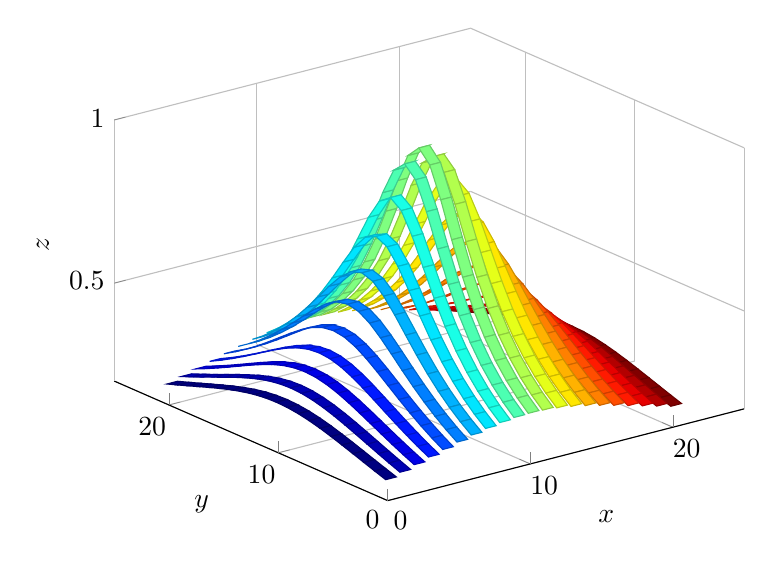
\begin{tikzpicture}

\begin{axis}[%
width=8cm,
height=6cm,
view={-37.5}{30},
scale only axis,
xmin=0,
xmax=25,
xlabel={\(x\)},
xmajorgrids,
ymin=0,
ymax=25,
ylabel={\(y\)},
ymajorgrids,
zmin=0.2,
zmax=1,
zlabel={\(z\)},
zmajorgrids,
axis x line*=bottom,
axis y line*=left,
axis z line*=left,
xticklabel style={/pgf/number format/assume math mode},
yticklabel style={/pgf/number format/assume math mode},
zticklabel style={/pgf/number format/assume math mode}
]

\addplot3[%
surf,
colormap/jet,
shader=faceted,
draw=black,
point meta=explicit,
mesh/rows=2]
table[row sep=crcr,meta index=3,header=false] {
20.625 1 0.242535625036333 21\\
20.625 2 0.254164283887674 21\\
20.625 3 0.266123147706175 21\\
20.625 4 0.278207442037329 21\\
20.625 5 0.29012942659283 21\\
20.625 6 0.301511344577764 21\\
20.625 7 0.311891430775903 21\\
20.625 8 0.320750149549792 21\\
20.625 9 0.327560891040209 21\\
20.625 10 0.331861655799986 21\\
20.625 11 0.333333333333333 21\\
20.625 12 0.331861655799986 21\\
20.625 13 0.327560891040209 21\\
20.625 14 0.320750149549792 21\\
20.625 15 0.311891430775903 21\\
20.625 16 0.301511344577764 21\\
20.625 17 0.29012942659283 21\\
20.625 18 0.278207442037329 21\\
20.625 19 0.266123147706175 21\\
20.625 20 0.254164283887674 21\\
20.625 21 0.242535625036333 21\\
21.375 1 0.242535625036333 21\\
21.375 2 0.254164283887674 21\\
21.375 3 0.266123147706175 21\\
21.375 4 0.278207442037329 21\\
21.375 5 0.29012942659283 21\\
21.375 6 0.301511344577764 21\\
21.375 7 0.311891430775903 21\\
21.375 8 0.320750149549792 21\\
21.375 9 0.327560891040209 21\\
21.375 10 0.331861655799986 21\\
21.375 11 0.333333333333333 21\\
21.375 12 0.331861655799986 21\\
21.375 13 0.327560891040209 21\\
21.375 14 0.320750149549792 21\\
21.375 15 0.311891430775903 21\\
21.375 16 0.301511344577764 21\\
21.375 17 0.29012942659283 21\\
21.375 18 0.278207442037329 21\\
21.375 19 0.266123147706175 21\\
21.375 20 0.254164283887674 21\\
21.375 21 0.242535625036333 21\\
};

\addplot3[%
surf,
colormap/jet,
shader=faceted,
draw=black,
point meta=explicit,
mesh/rows=2]
table[row sep=crcr,meta index=3,header=false] {
19.625 1 0.254164283887674 20\\
19.625 2 0.267643863786095 20\\
19.625 3 0.281718084909506 20\\
19.625 4 0.296174438879546 20\\
19.625 5 0.3106848830006 20\\
19.625 6 0.324784901230815 20\\
19.625 7 0.337868689199743 20\\
19.625 8 0.349215147884789 20\\
19.625 9 0.358057437019716 20\\
19.625 10 0.363696483726654 20\\
19.625 11 0.365636212063565 20\\
19.625 12 0.363696483726654 20\\
19.625 13 0.358057437019716 20\\
19.625 14 0.349215147884789 20\\
19.625 15 0.337868689199743 20\\
19.625 16 0.324784901230815 20\\
19.625 17 0.3106848830006 20\\
19.625 18 0.296174438879546 20\\
19.625 19 0.281718084909506 20\\
19.625 20 0.267643863786095 20\\
19.625 21 0.254164283887674 20\\
20.375 1 0.254164283887674 20\\
20.375 2 0.267643863786095 20\\
20.375 3 0.281718084909506 20\\
20.375 4 0.296174438879546 20\\
20.375 5 0.3106848830006 20\\
20.375 6 0.324784901230815 20\\
20.375 7 0.337868689199743 20\\
20.375 8 0.349215147884789 20\\
20.375 9 0.358057437019716 20\\
20.375 10 0.363696483726654 20\\
20.375 11 0.365636212063565 20\\
20.375 12 0.363696483726654 20\\
20.375 13 0.358057437019716 20\\
20.375 14 0.349215147884789 20\\
20.375 15 0.337868689199743 20\\
20.375 16 0.324784901230815 20\\
20.375 17 0.3106848830006 20\\
20.375 18 0.296174438879546 20\\
20.375 19 0.281718084909506 20\\
20.375 20 0.267643863786095 20\\
20.375 21 0.254164283887674 20\\
};

\addplot3[%
surf,
colormap/jet,
shader=faceted,
draw=black,
point meta=explicit,
mesh/rows=2]
table[row sep=crcr,meta index=3,header=false] {
18.625 1 0.266123147706175 19\\
18.625 2 0.281718084909506 19\\
18.625 3 0.298274993135947 19\\
18.625 4 0.315597201548902 19\\
18.625 5 0.333333333333333 19\\
18.625 6 0.350931203171798 19\\
18.625 7 0.367607311046904 19\\
18.625 8 0.382359556450936 19\\
18.625 9 0.39405520311955 19\\
18.625 10 0.401609664451249 19\\
18.625 11 0.404226041727222 19\\
18.625 12 0.401609664451249 19\\
18.625 13 0.39405520311955 19\\
18.625 14 0.382359556450936 19\\
18.625 15 0.367607311046904 19\\
18.625 16 0.350931203171798 19\\
18.625 17 0.333333333333333 19\\
18.625 18 0.315597201548902 19\\
18.625 19 0.298274993135947 19\\
18.625 20 0.281718084909506 19\\
18.625 21 0.266123147706175 19\\
19.375 1 0.266123147706175 19\\
19.375 2 0.281718084909506 19\\
19.375 3 0.298274993135947 19\\
19.375 4 0.315597201548902 19\\
19.375 5 0.333333333333333 19\\
19.375 6 0.350931203171798 19\\
19.375 7 0.367607311046904 19\\
19.375 8 0.382359556450936 19\\
19.375 9 0.39405520311955 19\\
19.375 10 0.401609664451249 19\\
19.375 11 0.404226041727222 19\\
19.375 12 0.401609664451249 19\\
19.375 13 0.39405520311955 19\\
19.375 14 0.382359556450936 19\\
19.375 15 0.367607311046904 19\\
19.375 16 0.350931203171798 19\\
19.375 17 0.333333333333333 19\\
19.375 18 0.315597201548902 19\\
19.375 19 0.298274993135947 19\\
19.375 20 0.281718084909506 19\\
19.375 21 0.266123147706175 19\\
};

\addplot3[%
surf,
colormap/jet,
shader=faceted,
draw=black,
point meta=explicit,
mesh/rows=2]
table[row sep=crcr,meta index=3,header=false] {
17.625 1 0.278207442037329 18\\
17.625 2 0.296174438879546 18\\
17.625 3 0.315597201548902 18\\
17.625 4 0.336336396998156 18\\
17.625 5 0.358057437019716 18\\
17.625 6 0.380142960634853 18\\
17.625 7 0.401609664451249 18\\
17.625 8 0.421075960533259 18\\
17.625 9 0.436852028330519 18\\
17.625 10 0.447213595499958 18\\
17.625 11 0.450834817333716 18\\
17.625 12 0.447213595499958 18\\
17.625 13 0.436852028330519 18\\
17.625 14 0.421075960533259 18\\
17.625 15 0.401609664451249 18\\
17.625 16 0.380142960634853 18\\
17.625 17 0.358057437019716 18\\
17.625 18 0.336336396998156 18\\
17.625 19 0.315597201548902 18\\
17.625 20 0.296174438879546 18\\
17.625 21 0.278207442037329 18\\
18.375 1 0.278207442037329 18\\
18.375 2 0.296174438879546 18\\
18.375 3 0.315597201548902 18\\
18.375 4 0.336336396998156 18\\
18.375 5 0.358057437019716 18\\
18.375 6 0.380142960634853 18\\
18.375 7 0.401609664451249 18\\
18.375 8 0.421075960533259 18\\
18.375 9 0.436852028330519 18\\
18.375 10 0.447213595499958 18\\
18.375 11 0.450834817333716 18\\
18.375 12 0.447213595499958 18\\
18.375 13 0.436852028330519 18\\
18.375 14 0.421075960533259 18\\
18.375 15 0.401609664451249 18\\
18.375 16 0.380142960634853 18\\
18.375 17 0.358057437019716 18\\
18.375 18 0.336336396998156 18\\
18.375 19 0.315597201548902 18\\
18.375 20 0.296174438879546 18\\
18.375 21 0.278207442037329 18\\
};

\addplot3[%
surf,
colormap/jet,
shader=faceted,
draw=black,
point meta=explicit,
mesh/rows=2]
table[row sep=crcr,meta index=3,header=false] {
16.625 1 0.29012942659283 17\\
16.625 2 0.3106848830006 17\\
16.625 3 0.333333333333333 17\\
16.625 4 0.358057437019716 17\\
16.625 5 0.384615384615385 17\\
16.625 6 0.412393049421161 17\\
16.625 7 0.440225453162812 17\\
16.625 8 0.466252404120157 17\\
16.625 9 0.487950036474267 17\\
16.625 10 0.502518907629606 17\\
16.625 11 0.50767308256681 17\\
16.625 12 0.502518907629606 17\\
16.625 13 0.487950036474267 17\\
16.625 14 0.466252404120157 17\\
16.625 15 0.440225453162812 17\\
16.625 16 0.412393049421161 17\\
16.625 17 0.384615384615385 17\\
16.625 18 0.358057437019716 17\\
16.625 19 0.333333333333333 17\\
16.625 20 0.3106848830006 17\\
16.625 21 0.29012942659283 17\\
17.375 1 0.29012942659283 17\\
17.375 2 0.3106848830006 17\\
17.375 3 0.333333333333333 17\\
17.375 4 0.358057437019716 17\\
17.375 5 0.384615384615385 17\\
17.375 6 0.412393049421161 17\\
17.375 7 0.440225453162812 17\\
17.375 8 0.466252404120157 17\\
17.375 9 0.487950036474267 17\\
17.375 10 0.502518907629606 17\\
17.375 11 0.50767308256681 17\\
17.375 12 0.502518907629606 17\\
17.375 13 0.487950036474267 17\\
17.375 14 0.466252404120157 17\\
17.375 15 0.440225453162812 17\\
17.375 16 0.412393049421161 17\\
17.375 17 0.384615384615385 17\\
17.375 18 0.358057437019716 17\\
17.375 19 0.333333333333333 17\\
17.375 20 0.3106848830006 17\\
17.375 21 0.29012942659283 17\\
};

\addplot3[%
surf,
colormap/jet,
shader=faceted,
draw=black,
point meta=explicit,
mesh/rows=2]
table[row sep=crcr,meta index=3,header=false] {
15.625 1 0.301511344577764 16\\
15.625 2 0.324784901230815 16\\
15.625 3 0.350931203171798 16\\
15.625 4 0.380142960634853 16\\
15.625 5 0.412393049421161 16\\
15.625 6 0.447213595499958 16\\
15.625 7 0.483368244522832 16\\
15.625 8 0.518475847365213 16\\
15.625 9 0.548821299948452 16\\
15.625 10 0.56980288229819 16\\
15.625 11 0.577350269189626 16\\
15.625 12 0.56980288229819 16\\
15.625 13 0.548821299948452 16\\
15.625 14 0.518475847365213 16\\
15.625 15 0.483368244522832 16\\
15.625 16 0.447213595499958 16\\
15.625 17 0.412393049421161 16\\
15.625 18 0.380142960634853 16\\
15.625 19 0.350931203171798 16\\
15.625 20 0.324784901230815 16\\
15.625 21 0.301511344577764 16\\
16.375 1 0.301511344577764 16\\
16.375 2 0.324784901230815 16\\
16.375 3 0.350931203171798 16\\
16.375 4 0.380142960634853 16\\
16.375 5 0.412393049421161 16\\
16.375 6 0.447213595499958 16\\
16.375 7 0.483368244522832 16\\
16.375 8 0.518475847365213 16\\
16.375 9 0.548821299948452 16\\
16.375 10 0.56980288229819 16\\
16.375 11 0.577350269189626 16\\
16.375 12 0.56980288229819 16\\
16.375 13 0.548821299948452 16\\
16.375 14 0.518475847365213 16\\
16.375 15 0.483368244522832 16\\
16.375 16 0.447213595499958 16\\
16.375 17 0.412393049421161 16\\
16.375 18 0.380142960634853 16\\
16.375 19 0.350931203171798 16\\
16.375 20 0.324784901230815 16\\
16.375 21 0.301511344577764 16\\
};

\addplot3[%
surf,
colormap/jet,
shader=faceted,
draw=black,
point meta=explicit,
mesh/rows=2]
table[row sep=crcr,meta index=3,header=false] {
14.625 1 0.311891430775903 15\\
14.625 2 0.337868689199743 15\\
14.625 3 0.367607311046904 15\\
14.625 4 0.401609664451249 15\\
14.625 5 0.440225453162812 15\\
14.625 6 0.483368244522832 15\\
14.625 7 0.52999894000318 15\\
14.625 8 0.577350269189626 15\\
14.625 9 0.620173672946042 15\\
14.625 10 0.650944554904119 15\\
14.625 11 0.662266178532522 15\\
14.625 12 0.650944554904119 15\\
14.625 13 0.620173672946042 15\\
14.625 14 0.577350269189626 15\\
14.625 15 0.52999894000318 15\\
14.625 16 0.483368244522832 15\\
14.625 17 0.440225453162812 15\\
14.625 18 0.401609664451249 15\\
14.625 19 0.367607311046904 15\\
14.625 20 0.337868689199743 15\\
14.625 21 0.311891430775903 15\\
15.375 1 0.311891430775903 15\\
15.375 2 0.337868689199743 15\\
15.375 3 0.367607311046904 15\\
15.375 4 0.401609664451249 15\\
15.375 5 0.440225453162812 15\\
15.375 6 0.483368244522832 15\\
15.375 7 0.52999894000318 15\\
15.375 8 0.577350269189626 15\\
15.375 9 0.620173672946042 15\\
15.375 10 0.650944554904119 15\\
15.375 11 0.662266178532522 15\\
15.375 12 0.650944554904119 15\\
15.375 13 0.620173672946042 15\\
15.375 14 0.577350269189626 15\\
15.375 15 0.52999894000318 15\\
15.375 16 0.483368244522832 15\\
15.375 17 0.440225453162812 15\\
15.375 18 0.401609664451249 15\\
15.375 19 0.367607311046904 15\\
15.375 20 0.337868689199743 15\\
15.375 21 0.311891430775903 15\\
};

\addplot3[%
surf,
colormap/jet,
shader=faceted,
draw=black,
point meta=explicit,
mesh/rows=2]
table[row sep=crcr,meta index=3,header=false] {
13.625 1 0.320750149549792 14\\
13.625 2 0.349215147884789 14\\
13.625 3 0.382359556450936 14\\
13.625 4 0.421075960533259 14\\
13.625 5 0.466252404120157 14\\
13.625 6 0.518475847365213 14\\
13.625 7 0.577350269189626 14\\
13.625 8 0.64018439966448 14\\
13.625 9 0.700140042014005 14\\
13.625 10 0.74535599249993 14\\
13.625 11 0.762492851663023 14\\
13.625 12 0.74535599249993 14\\
13.625 13 0.700140042014005 14\\
13.625 14 0.64018439966448 14\\
13.625 15 0.577350269189626 14\\
13.625 16 0.518475847365213 14\\
13.625 17 0.466252404120157 14\\
13.625 18 0.421075960533259 14\\
13.625 19 0.382359556450936 14\\
13.625 20 0.349215147884789 14\\
13.625 21 0.320750149549792 14\\
14.375 1 0.320750149549792 14\\
14.375 2 0.349215147884789 14\\
14.375 3 0.382359556450936 14\\
14.375 4 0.421075960533259 14\\
14.375 5 0.466252404120157 14\\
14.375 6 0.518475847365213 14\\
14.375 7 0.577350269189626 14\\
14.375 8 0.64018439966448 14\\
14.375 9 0.700140042014005 14\\
14.375 10 0.74535599249993 14\\
14.375 11 0.762492851663023 14\\
14.375 12 0.74535599249993 14\\
14.375 13 0.700140042014005 14\\
14.375 14 0.64018439966448 14\\
14.375 15 0.577350269189626 14\\
14.375 16 0.518475847365213 14\\
14.375 17 0.466252404120157 14\\
14.375 18 0.421075960533259 14\\
14.375 19 0.382359556450936 14\\
14.375 20 0.349215147884789 14\\
14.375 21 0.320750149549792 14\\
};

\addplot3[%
surf,
colormap/jet,
shader=faceted,
draw=black,
point meta=explicit,
mesh/rows=2]
table[row sep=crcr,meta index=3,header=false] {
12.625 1 0.327560891040209 13\\
12.625 2 0.358057437019716 13\\
12.625 3 0.39405520311955 13\\
12.625 4 0.436852028330519 13\\
12.625 5 0.487950036474267 13\\
12.625 6 0.548821299948452 13\\
12.625 7 0.620173672946042 13\\
12.625 8 0.700140042014005 13\\
12.625 9 0.78086880944303 13\\
12.625 10 0.845154254728517 13\\
12.625 11 0.870388279778489 13\\
12.625 12 0.845154254728517 13\\
12.625 13 0.78086880944303 13\\
12.625 14 0.700140042014005 13\\
12.625 15 0.620173672946042 13\\
12.625 16 0.548821299948452 13\\
12.625 17 0.487950036474267 13\\
12.625 18 0.436852028330519 13\\
12.625 19 0.39405520311955 13\\
12.625 20 0.358057437019716 13\\
12.625 21 0.327560891040209 13\\
13.375 1 0.327560891040209 13\\
13.375 2 0.358057437019716 13\\
13.375 3 0.39405520311955 13\\
13.375 4 0.436852028330519 13\\
13.375 5 0.487950036474267 13\\
13.375 6 0.548821299948452 13\\
13.375 7 0.620173672946042 13\\
13.375 8 0.700140042014005 13\\
13.375 9 0.78086880944303 13\\
13.375 10 0.845154254728517 13\\
13.375 11 0.870388279778489 13\\
13.375 12 0.845154254728517 13\\
13.375 13 0.78086880944303 13\\
13.375 14 0.700140042014005 13\\
13.375 15 0.620173672946042 13\\
13.375 16 0.548821299948452 13\\
13.375 17 0.487950036474267 13\\
13.375 18 0.436852028330519 13\\
13.375 19 0.39405520311955 13\\
13.375 20 0.358057437019716 13\\
13.375 21 0.327560891040209 13\\
};

\addplot3[%
surf,
colormap/jet,
shader=faceted,
draw=black,
point meta=explicit,
mesh/rows=2]
table[row sep=crcr,meta index=3,header=false] {
11.625 1 0.331861655799986 12\\
11.625 2 0.363696483726654 12\\
11.625 3 0.401609664451249 12\\
11.625 4 0.447213595499958 12\\
11.625 5 0.502518907629606 12\\
11.625 6 0.56980288229819 12\\
11.625 7 0.650944554904119 12\\
11.625 8 0.74535599249993 12\\
11.625 9 0.845154254728517 12\\
11.625 10 0.928476690885259 12\\
11.625 11 0.962250448649376 12\\
11.625 12 0.928476690885259 12\\
11.625 13 0.845154254728517 12\\
11.625 14 0.74535599249993 12\\
11.625 15 0.650944554904119 12\\
11.625 16 0.56980288229819 12\\
11.625 17 0.502518907629606 12\\
11.625 18 0.447213595499958 12\\
11.625 19 0.401609664451249 12\\
11.625 20 0.363696483726654 12\\
11.625 21 0.331861655799986 12\\
12.375 1 0.331861655799986 12\\
12.375 2 0.363696483726654 12\\
12.375 3 0.401609664451249 12\\
12.375 4 0.447213595499958 12\\
12.375 5 0.502518907629606 12\\
12.375 6 0.56980288229819 12\\
12.375 7 0.650944554904119 12\\
12.375 8 0.74535599249993 12\\
12.375 9 0.845154254728517 12\\
12.375 10 0.928476690885259 12\\
12.375 11 0.962250448649376 12\\
12.375 12 0.928476690885259 12\\
12.375 13 0.845154254728517 12\\
12.375 14 0.74535599249993 12\\
12.375 15 0.650944554904119 12\\
12.375 16 0.56980288229819 12\\
12.375 17 0.502518907629606 12\\
12.375 18 0.447213595499958 12\\
12.375 19 0.401609664451249 12\\
12.375 20 0.363696483726654 12\\
12.375 21 0.331861655799986 12\\
};

\addplot3[%
surf,
colormap/jet,
shader=faceted,
draw=black,
point meta=explicit,
mesh/rows=2]
table[row sep=crcr,meta index=3,header=false] {
10.625 1 0.333333333333333 11\\
10.625 2 0.365636212063565 11\\
10.625 3 0.404226041727222 11\\
10.625 4 0.450834817333716 11\\
10.625 5 0.50767308256681 11\\
10.625 6 0.577350269189626 11\\
10.625 7 0.662266178532522 11\\
10.625 8 0.762492851663023 11\\
10.625 9 0.870388279778489 11\\
10.625 10 0.962250448649376 11\\
10.625 11 1 11\\
10.625 12 0.962250448649376 11\\
10.625 13 0.870388279778489 11\\
10.625 14 0.762492851663023 11\\
10.625 15 0.662266178532522 11\\
10.625 16 0.577350269189626 11\\
10.625 17 0.50767308256681 11\\
10.625 18 0.450834817333716 11\\
10.625 19 0.404226041727222 11\\
10.625 20 0.365636212063565 11\\
10.625 21 0.333333333333333 11\\
11.375 1 0.333333333333333 11\\
11.375 2 0.365636212063565 11\\
11.375 3 0.404226041727222 11\\
11.375 4 0.450834817333716 11\\
11.375 5 0.50767308256681 11\\
11.375 6 0.577350269189626 11\\
11.375 7 0.662266178532522 11\\
11.375 8 0.762492851663023 11\\
11.375 9 0.870388279778489 11\\
11.375 10 0.962250448649376 11\\
11.375 11 1 11\\
11.375 12 0.962250448649376 11\\
11.375 13 0.870388279778489 11\\
11.375 14 0.762492851663023 11\\
11.375 15 0.662266178532522 11\\
11.375 16 0.577350269189626 11\\
11.375 17 0.50767308256681 11\\
11.375 18 0.450834817333716 11\\
11.375 19 0.404226041727222 11\\
11.375 20 0.365636212063565 11\\
11.375 21 0.333333333333333 11\\
};

\addplot3[%
surf,
colormap/jet,
shader=faceted,
draw=black,
point meta=explicit,
mesh/rows=2]
table[row sep=crcr,meta index=3,header=false] {
9.625 1 0.331861655799986 10\\
9.625 2 0.363696483726654 10\\
9.625 3 0.401609664451249 10\\
9.625 4 0.447213595499958 10\\
9.625 5 0.502518907629606 10\\
9.625 6 0.56980288229819 10\\
9.625 7 0.650944554904119 10\\
9.625 8 0.74535599249993 10\\
9.625 9 0.845154254728517 10\\
9.625 10 0.928476690885259 10\\
9.625 11 0.962250448649376 10\\
9.625 12 0.928476690885259 10\\
9.625 13 0.845154254728517 10\\
9.625 14 0.74535599249993 10\\
9.625 15 0.650944554904119 10\\
9.625 16 0.56980288229819 10\\
9.625 17 0.502518907629606 10\\
9.625 18 0.447213595499958 10\\
9.625 19 0.401609664451249 10\\
9.625 20 0.363696483726654 10\\
9.625 21 0.331861655799986 10\\
10.375 1 0.331861655799986 10\\
10.375 2 0.363696483726654 10\\
10.375 3 0.401609664451249 10\\
10.375 4 0.447213595499958 10\\
10.375 5 0.502518907629606 10\\
10.375 6 0.56980288229819 10\\
10.375 7 0.650944554904119 10\\
10.375 8 0.74535599249993 10\\
10.375 9 0.845154254728517 10\\
10.375 10 0.928476690885259 10\\
10.375 11 0.962250448649376 10\\
10.375 12 0.928476690885259 10\\
10.375 13 0.845154254728517 10\\
10.375 14 0.74535599249993 10\\
10.375 15 0.650944554904119 10\\
10.375 16 0.56980288229819 10\\
10.375 17 0.502518907629606 10\\
10.375 18 0.447213595499958 10\\
10.375 19 0.401609664451249 10\\
10.375 20 0.363696483726654 10\\
10.375 21 0.331861655799986 10\\
};

\addplot3[%
surf,
colormap/jet,
shader=faceted,
draw=black,
point meta=explicit,
mesh/rows=2]
table[row sep=crcr,meta index=3,header=false] {
8.625 1 0.327560891040209 9\\
8.625 2 0.358057437019716 9\\
8.625 3 0.39405520311955 9\\
8.625 4 0.436852028330519 9\\
8.625 5 0.487950036474267 9\\
8.625 6 0.548821299948452 9\\
8.625 7 0.620173672946042 9\\
8.625 8 0.700140042014005 9\\
8.625 9 0.78086880944303 9\\
8.625 10 0.845154254728517 9\\
8.625 11 0.870388279778489 9\\
8.625 12 0.845154254728517 9\\
8.625 13 0.78086880944303 9\\
8.625 14 0.700140042014005 9\\
8.625 15 0.620173672946042 9\\
8.625 16 0.548821299948452 9\\
8.625 17 0.487950036474267 9\\
8.625 18 0.436852028330519 9\\
8.625 19 0.39405520311955 9\\
8.625 20 0.358057437019716 9\\
8.625 21 0.327560891040209 9\\
9.375 1 0.327560891040209 9\\
9.375 2 0.358057437019716 9\\
9.375 3 0.39405520311955 9\\
9.375 4 0.436852028330519 9\\
9.375 5 0.487950036474267 9\\
9.375 6 0.548821299948452 9\\
9.375 7 0.620173672946042 9\\
9.375 8 0.700140042014005 9\\
9.375 9 0.78086880944303 9\\
9.375 10 0.845154254728517 9\\
9.375 11 0.870388279778489 9\\
9.375 12 0.845154254728517 9\\
9.375 13 0.78086880944303 9\\
9.375 14 0.700140042014005 9\\
9.375 15 0.620173672946042 9\\
9.375 16 0.548821299948452 9\\
9.375 17 0.487950036474267 9\\
9.375 18 0.436852028330519 9\\
9.375 19 0.39405520311955 9\\
9.375 20 0.358057437019716 9\\
9.375 21 0.327560891040209 9\\
};

\addplot3[%
surf,
colormap/jet,
shader=faceted,
draw=black,
point meta=explicit,
mesh/rows=2]
table[row sep=crcr,meta index=3,header=false] {
7.625 1 0.320750149549792 8\\
7.625 2 0.349215147884789 8\\
7.625 3 0.382359556450936 8\\
7.625 4 0.421075960533259 8\\
7.625 5 0.466252404120157 8\\
7.625 6 0.518475847365213 8\\
7.625 7 0.577350269189626 8\\
7.625 8 0.64018439966448 8\\
7.625 9 0.700140042014005 8\\
7.625 10 0.74535599249993 8\\
7.625 11 0.762492851663023 8\\
7.625 12 0.74535599249993 8\\
7.625 13 0.700140042014005 8\\
7.625 14 0.64018439966448 8\\
7.625 15 0.577350269189626 8\\
7.625 16 0.518475847365213 8\\
7.625 17 0.466252404120157 8\\
7.625 18 0.421075960533259 8\\
7.625 19 0.382359556450936 8\\
7.625 20 0.349215147884789 8\\
7.625 21 0.320750149549792 8\\
8.375 1 0.320750149549792 8\\
8.375 2 0.349215147884789 8\\
8.375 3 0.382359556450936 8\\
8.375 4 0.421075960533259 8\\
8.375 5 0.466252404120157 8\\
8.375 6 0.518475847365213 8\\
8.375 7 0.577350269189626 8\\
8.375 8 0.64018439966448 8\\
8.375 9 0.700140042014005 8\\
8.375 10 0.74535599249993 8\\
8.375 11 0.762492851663023 8\\
8.375 12 0.74535599249993 8\\
8.375 13 0.700140042014005 8\\
8.375 14 0.64018439966448 8\\
8.375 15 0.577350269189626 8\\
8.375 16 0.518475847365213 8\\
8.375 17 0.466252404120157 8\\
8.375 18 0.421075960533259 8\\
8.375 19 0.382359556450936 8\\
8.375 20 0.349215147884789 8\\
8.375 21 0.320750149549792 8\\
};

\addplot3[%
surf,
colormap/jet,
shader=faceted,
draw=black,
point meta=explicit,
mesh/rows=2]
table[row sep=crcr,meta index=3,header=false] {
6.625 1 0.311891430775903 7\\
6.625 2 0.337868689199743 7\\
6.625 3 0.367607311046904 7\\
6.625 4 0.401609664451249 7\\
6.625 5 0.440225453162812 7\\
6.625 6 0.483368244522832 7\\
6.625 7 0.52999894000318 7\\
6.625 8 0.577350269189626 7\\
6.625 9 0.620173672946042 7\\
6.625 10 0.650944554904119 7\\
6.625 11 0.662266178532522 7\\
6.625 12 0.650944554904119 7\\
6.625 13 0.620173672946042 7\\
6.625 14 0.577350269189626 7\\
6.625 15 0.52999894000318 7\\
6.625 16 0.483368244522832 7\\
6.625 17 0.440225453162812 7\\
6.625 18 0.401609664451249 7\\
6.625 19 0.367607311046904 7\\
6.625 20 0.337868689199743 7\\
6.625 21 0.311891430775903 7\\
7.375 1 0.311891430775903 7\\
7.375 2 0.337868689199743 7\\
7.375 3 0.367607311046904 7\\
7.375 4 0.401609664451249 7\\
7.375 5 0.440225453162812 7\\
7.375 6 0.483368244522832 7\\
7.375 7 0.52999894000318 7\\
7.375 8 0.577350269189626 7\\
7.375 9 0.620173672946042 7\\
7.375 10 0.650944554904119 7\\
7.375 11 0.662266178532522 7\\
7.375 12 0.650944554904119 7\\
7.375 13 0.620173672946042 7\\
7.375 14 0.577350269189626 7\\
7.375 15 0.52999894000318 7\\
7.375 16 0.483368244522832 7\\
7.375 17 0.440225453162812 7\\
7.375 18 0.401609664451249 7\\
7.375 19 0.367607311046904 7\\
7.375 20 0.337868689199743 7\\
7.375 21 0.311891430775903 7\\
};

\addplot3[%
surf,
colormap/jet,
shader=faceted,
draw=black,
point meta=explicit,
mesh/rows=2]
table[row sep=crcr,meta index=3,header=false] {
5.625 1 0.301511344577764 6\\
5.625 2 0.324784901230815 6\\
5.625 3 0.350931203171798 6\\
5.625 4 0.380142960634853 6\\
5.625 5 0.412393049421161 6\\
5.625 6 0.447213595499958 6\\
5.625 7 0.483368244522832 6\\
5.625 8 0.518475847365213 6\\
5.625 9 0.548821299948452 6\\
5.625 10 0.56980288229819 6\\
5.625 11 0.577350269189626 6\\
5.625 12 0.56980288229819 6\\
5.625 13 0.548821299948452 6\\
5.625 14 0.518475847365213 6\\
5.625 15 0.483368244522832 6\\
5.625 16 0.447213595499958 6\\
5.625 17 0.412393049421161 6\\
5.625 18 0.380142960634853 6\\
5.625 19 0.350931203171798 6\\
5.625 20 0.324784901230815 6\\
5.625 21 0.301511344577764 6\\
6.375 1 0.301511344577764 6\\
6.375 2 0.324784901230815 6\\
6.375 3 0.350931203171798 6\\
6.375 4 0.380142960634853 6\\
6.375 5 0.412393049421161 6\\
6.375 6 0.447213595499958 6\\
6.375 7 0.483368244522832 6\\
6.375 8 0.518475847365213 6\\
6.375 9 0.548821299948452 6\\
6.375 10 0.56980288229819 6\\
6.375 11 0.577350269189626 6\\
6.375 12 0.56980288229819 6\\
6.375 13 0.548821299948452 6\\
6.375 14 0.518475847365213 6\\
6.375 15 0.483368244522832 6\\
6.375 16 0.447213595499958 6\\
6.375 17 0.412393049421161 6\\
6.375 18 0.380142960634853 6\\
6.375 19 0.350931203171798 6\\
6.375 20 0.324784901230815 6\\
6.375 21 0.301511344577764 6\\
};

\addplot3[%
surf,
colormap/jet,
shader=faceted,
draw=black,
point meta=explicit,
mesh/rows=2]
table[row sep=crcr,meta index=3,header=false] {
4.625 1 0.29012942659283 5\\
4.625 2 0.3106848830006 5\\
4.625 3 0.333333333333333 5\\
4.625 4 0.358057437019716 5\\
4.625 5 0.384615384615385 5\\
4.625 6 0.412393049421161 5\\
4.625 7 0.440225453162812 5\\
4.625 8 0.466252404120157 5\\
4.625 9 0.487950036474267 5\\
4.625 10 0.502518907629606 5\\
4.625 11 0.50767308256681 5\\
4.625 12 0.502518907629606 5\\
4.625 13 0.487950036474267 5\\
4.625 14 0.466252404120157 5\\
4.625 15 0.440225453162812 5\\
4.625 16 0.412393049421161 5\\
4.625 17 0.384615384615385 5\\
4.625 18 0.358057437019716 5\\
4.625 19 0.333333333333333 5\\
4.625 20 0.3106848830006 5\\
4.625 21 0.29012942659283 5\\
5.375 1 0.29012942659283 5\\
5.375 2 0.3106848830006 5\\
5.375 3 0.333333333333333 5\\
5.375 4 0.358057437019716 5\\
5.375 5 0.384615384615385 5\\
5.375 6 0.412393049421161 5\\
5.375 7 0.440225453162812 5\\
5.375 8 0.466252404120157 5\\
5.375 9 0.487950036474267 5\\
5.375 10 0.502518907629606 5\\
5.375 11 0.50767308256681 5\\
5.375 12 0.502518907629606 5\\
5.375 13 0.487950036474267 5\\
5.375 14 0.466252404120157 5\\
5.375 15 0.440225453162812 5\\
5.375 16 0.412393049421161 5\\
5.375 17 0.384615384615385 5\\
5.375 18 0.358057437019716 5\\
5.375 19 0.333333333333333 5\\
5.375 20 0.3106848830006 5\\
5.375 21 0.29012942659283 5\\
};

\addplot3[%
surf,
colormap/jet,
shader=faceted,
draw=black,
point meta=explicit,
mesh/rows=2]
table[row sep=crcr,meta index=3,header=false] {
3.625 1 0.278207442037329 4\\
3.625 2 0.296174438879546 4\\
3.625 3 0.315597201548902 4\\
3.625 4 0.336336396998156 4\\
3.625 5 0.358057437019716 4\\
3.625 6 0.380142960634853 4\\
3.625 7 0.401609664451249 4\\
3.625 8 0.421075960533259 4\\
3.625 9 0.436852028330519 4\\
3.625 10 0.447213595499958 4\\
3.625 11 0.450834817333716 4\\
3.625 12 0.447213595499958 4\\
3.625 13 0.436852028330519 4\\
3.625 14 0.421075960533259 4\\
3.625 15 0.401609664451249 4\\
3.625 16 0.380142960634853 4\\
3.625 17 0.358057437019716 4\\
3.625 18 0.336336396998156 4\\
3.625 19 0.315597201548902 4\\
3.625 20 0.296174438879546 4\\
3.625 21 0.278207442037329 4\\
4.375 1 0.278207442037329 4\\
4.375 2 0.296174438879546 4\\
4.375 3 0.315597201548902 4\\
4.375 4 0.336336396998156 4\\
4.375 5 0.358057437019716 4\\
4.375 6 0.380142960634853 4\\
4.375 7 0.401609664451249 4\\
4.375 8 0.421075960533259 4\\
4.375 9 0.436852028330519 4\\
4.375 10 0.447213595499958 4\\
4.375 11 0.450834817333716 4\\
4.375 12 0.447213595499958 4\\
4.375 13 0.436852028330519 4\\
4.375 14 0.421075960533259 4\\
4.375 15 0.401609664451249 4\\
4.375 16 0.380142960634853 4\\
4.375 17 0.358057437019716 4\\
4.375 18 0.336336396998156 4\\
4.375 19 0.315597201548902 4\\
4.375 20 0.296174438879546 4\\
4.375 21 0.278207442037329 4\\
};

\addplot3[%
surf,
colormap/jet,
shader=faceted,
draw=black,
point meta=explicit,
mesh/rows=2]
table[row sep=crcr,meta index=3,header=false] {
2.625 1 0.266123147706175 3\\
2.625 2 0.281718084909506 3\\
2.625 3 0.298274993135947 3\\
2.625 4 0.315597201548902 3\\
2.625 5 0.333333333333333 3\\
2.625 6 0.350931203171798 3\\
2.625 7 0.367607311046904 3\\
2.625 8 0.382359556450936 3\\
2.625 9 0.39405520311955 3\\
2.625 10 0.401609664451249 3\\
2.625 11 0.404226041727222 3\\
2.625 12 0.401609664451249 3\\
2.625 13 0.39405520311955 3\\
2.625 14 0.382359556450936 3\\
2.625 15 0.367607311046904 3\\
2.625 16 0.350931203171798 3\\
2.625 17 0.333333333333333 3\\
2.625 18 0.315597201548902 3\\
2.625 19 0.298274993135947 3\\
2.625 20 0.281718084909506 3\\
2.625 21 0.266123147706175 3\\
3.375 1 0.266123147706175 3\\
3.375 2 0.281718084909506 3\\
3.375 3 0.298274993135947 3\\
3.375 4 0.315597201548902 3\\
3.375 5 0.333333333333333 3\\
3.375 6 0.350931203171798 3\\
3.375 7 0.367607311046904 3\\
3.375 8 0.382359556450936 3\\
3.375 9 0.39405520311955 3\\
3.375 10 0.401609664451249 3\\
3.375 11 0.404226041727222 3\\
3.375 12 0.401609664451249 3\\
3.375 13 0.39405520311955 3\\
3.375 14 0.382359556450936 3\\
3.375 15 0.367607311046904 3\\
3.375 16 0.350931203171798 3\\
3.375 17 0.333333333333333 3\\
3.375 18 0.315597201548902 3\\
3.375 19 0.298274993135947 3\\
3.375 20 0.281718084909506 3\\
3.375 21 0.266123147706175 3\\
};

\addplot3[%
surf,
colormap/jet,
shader=faceted,
draw=black,
point meta=explicit,
mesh/rows=2]
table[row sep=crcr,meta index=3,header=false] {
1.625 1 0.254164283887674 2\\
1.625 2 0.267643863786095 2\\
1.625 3 0.281718084909506 2\\
1.625 4 0.296174438879546 2\\
1.625 5 0.3106848830006 2\\
1.625 6 0.324784901230815 2\\
1.625 7 0.337868689199743 2\\
1.625 8 0.349215147884789 2\\
1.625 9 0.358057437019716 2\\
1.625 10 0.363696483726654 2\\
1.625 11 0.365636212063565 2\\
1.625 12 0.363696483726654 2\\
1.625 13 0.358057437019716 2\\
1.625 14 0.349215147884789 2\\
1.625 15 0.337868689199743 2\\
1.625 16 0.324784901230815 2\\
1.625 17 0.3106848830006 2\\
1.625 18 0.296174438879546 2\\
1.625 19 0.281718084909506 2\\
1.625 20 0.267643863786095 2\\
1.625 21 0.254164283887674 2\\
2.375 1 0.254164283887674 2\\
2.375 2 0.267643863786095 2\\
2.375 3 0.281718084909506 2\\
2.375 4 0.296174438879546 2\\
2.375 5 0.3106848830006 2\\
2.375 6 0.324784901230815 2\\
2.375 7 0.337868689199743 2\\
2.375 8 0.349215147884789 2\\
2.375 9 0.358057437019716 2\\
2.375 10 0.363696483726654 2\\
2.375 11 0.365636212063565 2\\
2.375 12 0.363696483726654 2\\
2.375 13 0.358057437019716 2\\
2.375 14 0.349215147884789 2\\
2.375 15 0.337868689199743 2\\
2.375 16 0.324784901230815 2\\
2.375 17 0.3106848830006 2\\
2.375 18 0.296174438879546 2\\
2.375 19 0.281718084909506 2\\
2.375 20 0.267643863786095 2\\
2.375 21 0.254164283887674 2\\
};

\addplot3[%
surf,
colormap/jet,
shader=faceted,
draw=black,
point meta=explicit,
mesh/rows=2]
table[row sep=crcr,meta index=3,header=false] {
0.625 1 0.242535625036333 1\\
0.625 2 0.254164283887674 1\\
0.625 3 0.266123147706175 1\\
0.625 4 0.278207442037329 1\\
0.625 5 0.29012942659283 1\\
0.625 6 0.301511344577764 1\\
0.625 7 0.311891430775903 1\\
0.625 8 0.320750149549792 1\\
0.625 9 0.327560891040209 1\\
0.625 10 0.331861655799986 1\\
0.625 11 0.333333333333333 1\\
0.625 12 0.331861655799986 1\\
0.625 13 0.327560891040209 1\\
0.625 14 0.320750149549792 1\\
0.625 15 0.311891430775903 1\\
0.625 16 0.301511344577764 1\\
0.625 17 0.29012942659283 1\\
0.625 18 0.278207442037329 1\\
0.625 19 0.266123147706175 1\\
0.625 20 0.254164283887674 1\\
0.625 21 0.242535625036333 1\\
1.375 1 0.242535625036333 1\\
1.375 2 0.254164283887674 1\\
1.375 3 0.266123147706175 1\\
1.375 4 0.278207442037329 1\\
1.375 5 0.29012942659283 1\\
1.375 6 0.301511344577764 1\\
1.375 7 0.311891430775903 1\\
1.375 8 0.320750149549792 1\\
1.375 9 0.327560891040209 1\\
1.375 10 0.331861655799986 1\\
1.375 11 0.333333333333333 1\\
1.375 12 0.331861655799986 1\\
1.375 13 0.327560891040209 1\\
1.375 14 0.320750149549792 1\\
1.375 15 0.311891430775903 1\\
1.375 16 0.301511344577764 1\\
1.375 17 0.29012942659283 1\\
1.375 18 0.278207442037329 1\\
1.375 19 0.266123147706175 1\\
1.375 20 0.254164283887674 1\\
1.375 21 0.242535625036333 1\\
};
\end{axis}
\end{tikzpicture}%

	\end{minipage}
	\\[1ex]
	\begin{minipage}{\textwidth}
		\begin{matlabcode}
% skapa lite exempeldata
[x, y] = meshgrid(-2:0.2:2,-2:0.2:2);
R = (1./((x+y).^2+(y-x).^2+1).^(1/2));
% plotta figuren
ribbon(R);
xlabel('x'); ylabel('y'); zlabel('z');
% spara figuren i tikz-format
matlab2tikz('figur.tex', 'width', '\textwidth', 'height', '.75\textwidth');
		\end{matlabcode}
	\end{minipage}
	\caption{\MATLAB-koden nederst genererar den \PGFTikZ-bild som
	syns överst.}
	\label{ex:tikzdevice}
\end{kod}

\subsubsubsection*{Från \Mathematica med ???}
\subsubsubsection*{Från \gnuplot med \TikZ-terminalen}

\subsubsection{Exportera i \PDF eller \PNG-fomat}
% Förklara; PDF>PNG eftersom vektorgrafik

\subsubsubsection*{Från \Rlogo till \PDF}
\Rlogo har ett antal inbyggda så kallade enheter \eng{device} som kan
användas för att rita diagram, grafer och liknande, bland annat för \EPS,
\PNG och \textsc{SVG} \parencite[\ppno~675–676]{RCoreTeam12}. Enheten vi är mest
intresserade av är den som producerar \PDF-filer. Denna används enkelt
genom att köra kommandot \texttt{pdf}, som tar samma parametrar som
\texttt{tikz}-kommandot som beskrevs tidigare. \PDF-filen som genereras
kan sedan enkelt inkluderas i ett \LaTeX-dokument med \cmd{includegraphics}.
\Cref{ex:pdfdevice} visar hur det kan se ut.

\begin{kod}[tbp]
	\centering
	\begin{minipage}{\textwidth}
		\centering
		\includegraphics{\latexbokFiguredir/4/pdfdevice.pdf}
	\end{minipage}
	\\[1ex]
	\begin{minipage}{\textwidth}
		\begin{rcode*}{mathescape=true}
# width och height specificeras i tum
pdf('figur.tex', width=4, height=2.5)
# exempel med ggplot2, som diskuteras på $\text{\cpageref{sec:ggplot2}}$
require(ggplot2)
ggplot(diamonds, aes(depth, fill = cut)) +
  + geom_density(alpha = 0.2) + xlim(55, 70)
# stäng $\text{\PDF}$-filen
dev.off()
		\end{rcode*}
	\end{minipage}
	\caption{\Rlogo-koden nederst genererar den \PDF-bild som
	syns överst.}
	\label{ex:pdfdevice}
\end{kod}

\subsubsubsection*{Från \MATLAB till \PNG}
% Att tänka på: http://tex.stackexchange.com/questions/5559/how-to-avoid-large-margins-around-matlab-plot-in-pdf
\subsubsubsection*{Från \Mathematica till \PDF}
% http://mathematica.stackexchange.com/a/750/1519
\subsubsubsection*{Från \gnuplot till \PDF}

\label{sec:4:end}
\end{document}
